% arara: xelatex
\documentclass[12pt]{article}

% \usepackage{physics} % это трэшовый пакет!

\usepackage{hyperref}
\hypersetup{
    colorlinks=true,
    linkcolor=blue,
    filecolor=magenta,      
    urlcolor=cyan,
    pdftitle={Overleaf Example},
    pdfpagemode=FullScreen,
    }
\urlstyle{same} % шрифт из основного текста

\usepackage{verse}

\usepackage{ulem} % перечёркнутый шрифт \sout{что-то} 

\usepackage{tikzducks}

\usepackage{tikz} % картинки в tikz
\usetikzlibrary{arrows.meta}
\usetikzlibrary{shapes, arrows, positioning}
\usepackage{tikz-3dplot} 
\usepackage{tkz-euclide}

\usepackage{verbatim}
\usepackage{microtype} % свешивание пунктуации

\usepackage{array} % для столбцов фиксированной ширины

\usepackage{indentfirst} % отступ в первом параграфе

\usepackage{sectsty} % для центрирования названий частей
\allsectionsfont{\centering}

\usepackage{amsmath, amsfonts, amssymb, amsthm} % куча стандартных математических плюшек

\usepackage{comment}

\usepackage[top=2cm, left=1.2cm, right=1.2cm, bottom=2cm]{geometry} % размер текста на странице

\usepackage{lastpage} % чтобы узнать номер последней страницы

\usepackage{enumitem} % дополнительные плюшки для списков
%  например \begin{enumerate}[resume] позволяет продолжить нумерацию в новом списке
\usepackage{caption}

\usepackage{url} % to use \url{link to web}

\newcommand{\smallduck}{\begin{tikzpicture}[scale=0.3]
    \duck[
        cape=black,
        hat=black,
        mask=black
    ]
    \end{tikzpicture}}

\usepackage{fancyhdr} % весёлые колонтитулы
\pagestyle{fancy}
\lhead{}
\chead{}
\rhead{}
\lfoot{}
\cfoot{}
\rfoot{}

\renewcommand{\headrulewidth}{0.4pt}
\renewcommand{\footrulewidth}{0.4pt}

\usepackage{tcolorbox} % рамочки!
\usepackage{graphicx} % рисунки
\usepackage{todonotes} % для вставки в документ заметок о том, что осталось сделать
% \todo[inline]{Здесь надо коэффициенты исправить}
% \missingfigure{Здесь будет Последний день Помпеи}
% \listoftodos - печатает все поставленные \todo'шки


% более красивые таблицы
\usepackage{booktabs}
% заповеди из докупентации:
% 1. Не используйте вертикальные линни
% 2. Не используйте двойные линии
% 3. Единицы измерения - в шапку таблицы
% 4. Не сокращайте .1 вместо 0.1
% 5. Повторяющееся значение повторяйте, а не говорите "то же"


\setcounter{MaxMatrixCols}{20}
% by crazy default pmatrix supports only 10 cols :)


\usepackage{fontspec}
\usepackage{libertine}
\usepackage{polyglossia}

\setmainlanguage{russian}
\setotherlanguages{english}

% download "Linux Libertine" fonts:
% http://www.linuxlibertine.org/index.php?id=91&L=1
% \setmainfont{Linux Libertine O} % or Helvetica, Arial, Cambria
% why do we need \newfontfamily:
% http://tex.stackexchange.com/questions/91507/
% \newfontfamily{\cyrillicfonttt}{Linux Libertine O}

\AddEnumerateCounter{\asbuk}{\russian@alph}{щ} % для списков с русскими буквами
\setlist[enumerate, 1]{label=\asbuk*),ref=\asbuk*}



\usepackage[bibencoding=auto, backend=biber, sorting=none, style=alphabetic]{biblatex}
\addbibresource{econometrics.bib}

\graphicspath{{./figures}}

%% эконометрические сокращения
\DeclareMathOperator{\IMR}{IMR} % Inverse Mill's ratio
\DeclareMathOperator{\Cov}{\mathbb{C}ov}
\DeclareMathOperator{\Corr}{\mathbb{C}orr}
\DeclareMathOperator{\sCov}{sCov}
\DeclareMathOperator{\sCorr}{sCorr}
\DeclareMathOperator{\sVar}{sVar}
\DeclareMathOperator{\Var}{\mathbb{V}ar}
\DeclareMathOperator{\hVar}{\widehat{\Var}}
\DeclareMathOperator{\hCov}{\widehat{\Cov}}
\DeclareMathOperator{\hCorr}{\widehat{\Corr}}
\DeclareMathOperator{\col}{col}
\DeclareMathOperator{\colspan}{colspan}

\DeclareMathOperator{\se}{se}
\DeclareMathOperator{\row}{row}
\DeclareMathOperator{\grad}{grad}
\DeclareMathOperator{\BestLin}{BestLin}

\let\P\relax
\DeclareMathOperator{\P}{\mathbb{P}}

\DeclareMathOperator{\E}{\mathbb{E}}
\DeclareMathOperator{\trace}{trace}
\DeclareMathOperator{\rank}{rank}
\DeclareMathOperator{\tr}{\trace}
\DeclareMathOperator{\rk}{\rank}
\DeclareMathOperator{\card}{card}
\DeclareMathOperator{\Span}{span}
% \span используется латехом для внутренних нужд

\DeclareMathOperator{\mgf}{mgf}

\DeclareMathOperator{\Convex}{Convex}
\DeclareMathOperator{\plim}{plim}

\usepackage{mathtools}
\DeclarePairedDelimiter{\norm}{\lVert}{\rVert}
\DeclarePairedDelimiter{\abs}{\lvert}{\rvert}
\DeclarePairedDelimiter{\scalp}{\langle}{\rangle}
\DeclarePairedDelimiter{\ceil}{\lceil}{\rceil}

% https://tex.stackexchange.com/questions/12910/how-do-i-typeset-vertical-and-horizontal-lines-inside-a-matrix
% для линий в матрицах
\newcommand*{\horzbar}{\rule[.5ex]{2.5ex}{0.5pt}}
\newcommand*{\vertbar}{\rule[-1ex]{0.5pt}{2.5ex}}


\newcommand{\cN}{\mathcal{N}}
\newcommand{\cF}{\mathcal{F}}

\newcommand{\RR}{\mathbb{R}}
\newcommand{\NN}{\mathbb{N}}

\newcommand{\dBern}{\mathrm{Bern}}
\newcommand{\dPois}{\mathrm{Pois}}
\newcommand{\dBin}{\mathrm{Bin}}
\newcommand{\dMult}{\mathrm{Mult}}
\newcommand{\dGeom}{\mathrm{Geom}}
\newcommand{\dNHGeom}{\mathrm{NHGeom}}
\newcommand{\dHGeom}{\mathrm{HGeom}}
\newcommand{\dDUnif}{\mathrm{DUnif}}
\newcommand{\dFS}{\mathrm{FS}}
\newcommand{\dNBin}{\mathrm{NBin}}

\newcommand{\dTri}{\mathrm{Triangle}}
\newcommand{\dUnif}{\mathrm{Unif}}
\newcommand{\dCauchy}{\mathrm{Cauchy}}
\newcommand{\dN}{\mathcal{N}}
\newcommand{\dLN}{\mathcal{LN}}
\newcommand{\dExpo}{\mathrm{Expo}}
\newcommand{\dBeta}{\mathrm{Beta}}
\newcommand{\dGamma}{\mathrm{Gamma}}
\newcommand{\dWei}{\mathrm{Wei}}
\newcommand{\dLogistic}{\mathrm{Logistic}}
\newcommand{\dRayleigh}{\mathrm{Rayleigh}}
\newcommand{\dPareto}{\mathrm{Pareto}}


% \renewcommand{\b}{\beta} % commented to avoid conflicts with base latex
% \renewcommand{\u}{u} % commented to avoid conflicts with base latex

\newcommand{\hb}{\hat{\beta}}
\newcommand{\tb}{\tilde{\beta}}
\newcommand{\hu}{\hat{u}}
\newcommand{\hs}{\hat{\sigma}}
\newcommand{\hy}{\hat{y}}
\newcommand{\one}{s} % обозначение для вектора (1, 1, 1, ..., 1). 
% s = ship forest, при желании можно заменить на \veс{1}

\newcommand{\RSS}{RSS}
\newcommand{\ESS}{ESS}
\newcommand{\TSS}{TSS}


\newcommand{\alt}{\text{alt}}
\newcommand{\adj}{\text{adj}}
\newcommand{\best}{\text{best}}
\newcommand{\ols}{\text{ols}}
\newcommand{\new}{\text{new}}
\newcommand{\old}{\text{old}}


% выделение питоновских и других пакетов
\newcommand{\sklearn}{sklearn}
\newcommand{\statsmodels}{statsmodels}



\newcommand{\gaussmarkov}{
\begin{enumerate}[label=\arabic*.]
    \item Модель линейна по параметрам: $y = X\beta + u$;
    \item Матрица $X$ размера $[n \times k]$ имеет полный ранг $k$.
    \item Условное ожидание ошибок равно нулю, $\E(u\mid X) = 0$;
    \item Условная ковариационная матрица ошибок пропорциональна единичной, $\Var(u\mid X) = \sigma^2 I$;
    \item Оценка $\hb$ получена методом наименьших квадратов, $\hb = (X^T X)^{-1}X^T y$;
\end{enumerate}}

\usepackage{thmtools} % тонкая настройка окружения теорем


% окружения!
\declaretheorem[
style=definition, 
%thmbox=M,
title=Теорема, 
numberwithin=section, 
]{theorem}


\declaretheorem[
style=definition, 
title=Утверждение, 
numberwithin=section, 
]{lemma}


\declaretheorem[
style=definition, 
title=Суть, 
numberwithin=section, 
]{explanation}



% опция sibling=theorem посередине даёт сквозную нумерацию с теоремами
\declaretheorem[
style=definition, 
title=Определение, 
sibling=theorem, 
]{definition}

\declaretheorem[
style=definition, 
title=Задача, 
% sibling=theorem, 
]{problem}


\declaretheorem[
style=definition,
title=Решение,
numbered=no
]{sol}


%\newenvironment{problem}{}{} % environment just prints the text
% \newenvironment{sol}{}{}
\newcommand{\trru}[1]{#1}
\newcommand{\tren}[1]{#1}



\begin{document}

% задачи можно дёргать:
% https://github.com/bdemeshev/metrics_pro/blob/master/metrics_body.tex
% и ещё (слегка модифицируя)
% https://github.com/bdemeshev/em_pset
% картиночки и доказательства на английском:
% https://github.com/olyagnilova/gauss-markov-pythagoras

\tableofcontents{}



\section{Методы получения оценок}

Методы получения оценок: метод максимального правдоподобия, метод моментов, метод наименьших квадратов.



\subsection{Задачи}
\begin{problem}
В оценках часто используют различные выражения с суммами. 
Пора перестать их бояться!
Проверьте, верны ли следующие формулы,
\begin{enumerate}
\item $\sum_{i=1}^n {(x_i-\bar x)} = 0$;
\item $\sum_{i=1}^n {(x_i-\bar x)^2} = \sum_{i=1}^n {(x_i-\bar x)x_i}$;
\item $\sum_{i=1}^n {(x_i-\bar x)(y_i-\bar y)} = \sum_{i=1}^n {(x_i-\bar x)y_i}$;
\item $\sum_{i=1}^n {(x_i-\bar x)(y_i-\bar y)} = \sum_{i=1}^n {x_i y_i}$;
\item $\sum_{i=1}^n x_i = n\bar x$;
\item $\sum_{i=1}^n (x_i - \bar x)^2 = \sum_{i=1}^n x_i^2 - n \bar x^2$;
\item $\sum_{i=1}^n (x_i - \bar x)(y_i - \bar y) = \sum_{i=1}^n x_i y_i - n \bar x \bar y$;
\item $\sum_{i=1}^n x_i^2 = \left( \sum_{i=1}^n x_i \right)^2$;
\item $\sum_{i=1}^n x_i^2 = (n\bar x)^2$;
\item $\sum_{i=1}^n \bar x = n \bar x$;
\item $\sum_{i=1}^n x_i \bar x = n \bar x^2$;
\item $\sum_{i=1}^n {(x_i-\bar x)y_i} = 0$.
\end{enumerate}

    \begin{sol}
        \todo[inline]{Здесь неотразимый ассист напишет решение}
    \end{sol}
\end{problem}





\section{Свойства оценок}
Свойства оценок: несмещённость, состоятельность, эффективность в классе.

\subsection{Практическое напоминание об условном ожидании и дисперсии}

Вспомним условное ожидание и условную дисперсию в дискретном случае:
\begin{problem}
Совместный закон распределения пары случайных величин $(x, y)$ задан таблицей:

\begin{tabular}{ccc}
\toprule
     & $y = 1$ & $y = 3$ \\
\midrule
$x = 1$ & 0.1 & 0.3 \\
$x = 2$ & 0.1 & 0.1 \\
$x = 4$ & 0.2 & 0.2 \\
\bottomrule
\end{tabular}

\begin{enumerate}
    \item Найдите $\E(y \mid x)$, $\Var(y \mid x)$.
    \item Найдите $\E(y)$, $\E(x)$, $\Cov(x, y)$, $\Var(x)$.
    \item Найдите наилучшее линейное приближение $\BestLin(y \mid x)$.
\end{enumerate}

    \begin{sol}
    \begin{enumerate}
    \item Условное математическое ожидание и дисперсия:
   \[
   \E(y \mid x) = \begin{cases}
   2.5, & x = 1, \\
   2, & x = 2, 4,
   \end{cases}
   \]
   \[
   \Var(y \mid x) = \begin{cases}
   0.75, & x = 1, \\
   1, & x = 2, 4.
   \end{cases}
   \]
    \item Математические ожидания, ковариация и дисперсия:
   \[
   \E(y) = 2.2, \quad \E(x) = 2.4, \quad \Cov(x, y) = -0.28, \quad \Var(x) = 1.84.
   \]
    \item Наилучшее линейное приближение:
   \[
   \BestLin(y \mid x) \approx 2.57 - 0.15 \cdot x.
   \]
   \end{enumerate}
    \end{sol}
\end{problem}

Теперь вспомним, как считать условные характеристики случайных величин при наличии совместной плотности:
\begin{problem}
Пара случайных величин $(x, y)$ имеет функцию плотности
\[
f(x, y) = \begin{cases}
(2x + 4y)/3, \text{ если } x\in [0, 1], y\in [0, 1], \\
0, \text{ иначе.}
\end{cases}
\]

\begin{enumerate}
    \item Найдите $\E(y \mid x)$, $\Var(y \mid x)$.
    \item Найдите $\E(y)$, $\E(x)$, $\Cov(x, y)$, $\Var(x)$.
    \item Найдите наилучшее линейное приближение $\BestLin(y \mid x)$.
\end{enumerate}

    \begin{sol}
        \todo[inline]{Здесь мудрый ассист напишет решение}
    \end{sol}
\end{problem}


Особо обратим внимание на случай двумерного нормального распределения:
\begin{problem}
Пара случайных величин $(x, y)$ имеет совместное нормальное распределение
\[
\begin{pmatrix}
    x \\
    y 
\end{pmatrix} \sim \cN\left(\begin{pmatrix}
    3 \\
    2 \\
\end{pmatrix}, 
\begin{pmatrix}
    10 & -2 \\
    -2 & 20
\end{pmatrix}\right)
\]

\begin{enumerate}
    \item Найдите $\E(y \mid x)$, $\Var(y \mid x)$.
    \item Найдите $\E(y)$, $\E(x)$, $\Cov(x, y)$, $\Var(x)$.
    \item Найдите наилучшее линейное приближение $\BestLin(y \mid x)$.
\end{enumerate}

    \begin{sol}
        \todo[inline]{Здесь храбрый ассист напишет решение}
    \end{sol}
\end{problem}

Обратите внимание: для совместного нормального распределения условное ожидание $\E(y \mid x)$ и наилучшее линейное приближение $\BestLin(y \mid x)$ идеально совпадают. 
Условное ожидание и линейное приближение совпадут и в том случае, если величина $x$ принимает всего два значения.
Убедимся в этом с помощью простой задачи

\begin{problem}
    На первом шаге Илон Маск случайным образом выбирает одно из двух значений случайной величины $x$, $\P(x = 1) = 0.4$, $\P(x = 2) = 0.6$.
    На втором шаге Шивон Зилис выбирает значение $y$ из экспоненциального распределения $x$ с интенсивностью $x$.

\begin{enumerate}
    \item Найдите $\E(y \mid x)$, $\Var(y \mid x)$.
    \item Найдите $\E(y)$, $\E(x)$, $\Cov(x, y)$, $\Var(x)$.
    \item Найдите наилучшее линейное приближение $\BestLin(y \mid x)$.
\end{enumerate}

    \begin{sol}
        \todo[inline]{Здесь неотразимый ассист напишет решение}
    \end{sol}
\end{problem}


Теперь найдём условное ожидание и условную дисперсию для совместного нормального распределения в общем виде. 



\begin{definition}[наилучшее линейное приближение]
\emph{Наилучшее линейное приближение} величины $r$ с помощью величины $s$ — это линейная функция от $s$,
\[
\BestLin(r \mid s) = \beta_1 + \beta_2 s,
\]
где константы $\beta_1$ и $\beta_2$ находятся из решения задачи оптимизации
$\E((r - \BestLin(r, s)^2) \to \min_{\beta_1, \beta_2}$.
При решении задачи окажется
\[
\beta_1 = \E(r) - \beta_2 \E(s), \quad \beta_2 = \frac{\Cov(r, s)}{\Var(s)}
\]
\end{definition}

\begin{definition}[линейно-независимые случайные величины]
Величины $r$ и $s$ называются \emph{линейно-независимыми}, если $\BestLin(r \mid s) = \E(r)$.
\end{definition}

Линейная независимость является симметричным явлением, $\BestLin(r \mid s) = \E(r)$, 
если и только если $\BestLin(s \mid r) = \E(s)$.


\begin{problem}
Выразите константы $\beta_1$ и $\beta_2$ в формуле для наилучшего линейного приближения 
\[
\BestLin(r \mid s) = \beta_1 + \beta_2 s,
\]
исходя из характеристик случайных величин $r$ и $s$. 

\begin{sol}
Выпишем целевую функцию в виде суммы
\[
    \E((r - \BestLin(r, s)^2)  = \Var(r - \beta_1- \beta_2 s) + (\E(r - \beta_1 - \beta_2 s))^2
\]
Заметим, что $\beta_1$ не влияет на первое слагаемое, так как дисперсия константы равна нулю.
И при этом, выбрав $\beta_1 = \E(r - \beta_2 s) = \E(r) - \beta_2\E(s)$ мы добьёмся того, что второе слагаемое будет равно нулю, своему наименьшему возможному значению. 

Остаётся минимизировать с помощью $\beta_2$ первое слагаемое. 
\[
\Var(r - \beta s) = \Var(r) + \beta_2^2 \Var(s) - 2 \beta_2 \Cov(r, s) \to \min_{\beta_2}.
\]
Перед нами квадратичная функция от $\beta_2$, следовательно, 
\[
\beta_2 = \frac{\Cov(r, s)}{ \Var(s)}.
\]
Обратите внимание, эта формула — родная «теоретическая» сестра «выборочной» формулы для парной регресcии
\[
\hb_2 = \frac{S_{xy}}{S_{xx}}.
\]
Аналогия между оценкой и истинным коэффициентом действует и для первого коэффициента,
\[
\beta_1 = \E(r) - \beta_2 \E(s), \quad  \hb_1 = \bar y - \hb_2 \bar x.
\]

И, попутно, мы замечаем, что условие $\Cov(r, s) = 0$ равносильно условию  $\BestLin(r \mid s) = \E(r)$ или условию $\BestLin(s \mid r) = \E(s)$.
\end{sol}
\end{problem}



\section{Асимптотические методы}
Центральная предельная теорема. Лемма Слуцкого. Дельта-метод. Построение асимптотических доверительных интервалов.


\section{Святая троица тестов}
Три классических теста: LM, LR, Wald.


Чёрный трек: тесты в матричной форме для вектора параметров?
\subsection{Черный трек}
\subsection{Тройка тестов в матричной форме}
Рассмотрим применение тестов W  (тест Вальда), LR (тест отношения правдоподобия) и LM (тест множителей Лагранжа) для тестирования гипотез о параметрах модели.

Пусть требуется протестировать систему ограничений относительно вектора неизвестных параметров
\[
H_0: \begin{cases}
g_1(\theta) = 0 \\
g_2(\theta) = 0 \\
\ldots \\
g_r(\theta) = 0 \\
\end{cases}
\]
где $g_i(\theta)$ — функция, которая задаёт $i$-е ограничение на вектор параметров $\theta$, $i = 1,\ldots, r$.

Введём следующие обозначения: 

\[
\frac{\partial g}{\partial \theta^T} = \begin{pmatrix}
\partial g_1/\partial \theta^T \\
\partial g_2/\partial \theta^T \\
\vdots \\
\partial g_r/\partial \theta^T \\
\end{pmatrix} = \begin{pmatrix}
\frac{\partial g_1}{\partial \theta_1} & \frac{\partial g_1}{\partial \theta_2} & \ldots & \frac{\partial g_1}{\partial \theta_k}\\
\frac{\partial g_2}{\partial \theta_1} & \frac{\partial g_2}{\partial \theta_2} & \ldots & \frac{\partial g_2}{\partial \theta_k}\\
\ldots & \ldots & \ldots & \ldots \\
\frac{\partial g_r}{\partial \theta_1} & \frac{\partial g_r}{\partial \theta_2} & \ldots & \frac{\partial g_r}{\partial \theta_k}\\
\end{pmatrix}
\]

\[
\frac{\partial g^T}{\partial \theta} = \begin{pmatrix}
\frac{\partial g^T_1}{\partial \theta} & \frac{\partial g^T_2}{\partial \theta} & \ldots & \frac{\partial g^T_r}{\partial \theta} \\
\end{pmatrix} = \begin{pmatrix}
\frac{\partial g_1}{\partial \theta_1} & \frac{\partial g_2}{\partial \theta_1} & \ldots & \frac{\partial g_r}{\partial \theta_1}\\
\frac{\partial g_1}{\partial \theta_2} & \frac{\partial g_2}{\partial \theta_2} & \ldots & \frac{\partial g_r}{\partial \theta_2}\\
\ldots & \ldots & \ldots & \ldots \\
\frac{\partial g_1}{\partial \theta_k} & \frac{\partial g_2}{\partial \theta_k} & \ldots & \frac{\partial g_r}{\partial \theta_k}\\
\end{pmatrix},  \frac{\partial \ell}{\partial \theta}= \begin{pmatrix}
\frac{\partial \ell}{\partial \theta_1} \\
\frac{\partial \ell}{\partial \theta_2} \\
\vdots \\
\frac{\partial \ell}{\partial \theta_k} \\
\end{pmatrix}
\]

\[
I(\theta) = -E \left(\frac{\partial^2 \ell}{\partial \theta \partial \theta^T}\right) = - \E \begin{pmatrix}
\frac{\partial^2 \ell}{\partial \theta_1 \partial \theta_1} & \frac{\partial^2 \ell}{\partial \theta_1 \partial \theta_2} & \ldots & \frac{\partial^2 \ell}{\partial \theta_1 \partial \theta_k} \\
\frac{\partial^2 \ell}{\partial \theta_2 \partial \theta_1} & \frac{\partial^2 \ell}{\partial \theta_2 \partial \theta_2} & \ldots & \frac{\partial^2 \ell}{\partial \theta_2 \partial \theta_k} \\
\ldots & \ldots & \ldots & \ldots \\
\frac{\partial^2 \ell}{\partial \theta_k \partial \theta_1} & \frac{\partial^2 \ell}{\partial \theta_k \partial \theta_2} & \ldots & \frac{\partial^2 \ell}{\partial \theta_k \partial \theta_k} 
\end{pmatrix}
\]
— информационная матрица Фишера

$\Theta_{UR} := \Theta$ — множество допустимых значений вектора неизвестных параметров без учёта ограничений

$\Theta_{R} := \{ \theta \in \Theta: g(\theta) = 0\}$ — множество допустимых значений вектора неизвестных параметров с учётом ограничений

$\hat{\theta}_{UR} \in \Theta_{UR}$ — точка максимума функции $\ell$ на множестве $\Theta_{UR}$

$\hat{\theta}_{R} \in \Theta_{R}$ — точка максимума функции $\ell$ на множестве $\Theta_{R}$

Тогда для тестирования гипотезы $H_0$ можно воспользоваться одной из следующих ниже статистик:

$LR := -2(\ell(\hat{\theta}_{R}) - \ell(\hat{\theta}_{UR})) \overset{as.}{\sim} \chi^2_r$ — статистика отношения правдоподобия

$W := g^T(\hat{\theta}_{UR}) \cdot \left[ \frac{\partial g}{\partial \theta^T}(\hat{\theta}_{UR}) \cdot I^{-1}(\hat{\theta}_{UR}) \cdot \frac{\partial g^T}{\partial \theta}(\hat{\theta}_{UR}) \right]^{-1} g(\hat{\theta}_{UR}) \overset{as.}{\sim} \chi^2_r$ — статистика Вальда

$LM := \left[ \frac{\partial \ell}{\partial \theta}(\hat{\theta}_{R}) \right]^T \cdot I^{-1}(\hat{\theta}_{R}) \cdot \left[ \frac{\partial \ell}{\partial \theta}(\hat{\theta}_{R}) \right] \overset{as.}{\sim} \chi^2_r$ — статистика множителей Лагранжа


\section{ШБ — МНК}

В этой главе мы приступим к изучению регрессионного анализа. Представьте, что вы работаете риэлтором или собираетесь приобрести квартиру в Москве. 
В обоих случаях Вас может интересовать, от чего зависит стоимость жилья (к примеру, 
от площади квартиры, расположения в том или ином районе Москвы и т.д.). Регрессионный анализ позволяет не только прогнозировать стоимость нового жилья, но и определять, какие факторы влияют на цену и в какую сторону — увеличивают или уменьшают её.

Для того чтобы корректно построить модель регрессии, сперва нам необходимо поставить оптимизационную задачу метода наименьших квадратов (МНК), найти её решение и обнаружить нестатистические свойства оценок. 


\subsection{Оптимизационная задача}\label{sec:optimization}
Моделью парной регрессии называется модель вида
\[
y_i = \beta_1 + \beta_2 x_i + u_i,
\]
где $y_i$ — значение зависимой (или, иначе, объясняемой) переменной для $i$-го наблюдения, $x_{i}$ — значение объясняющей переменной (иногда её называют фактором или регрессором, иногда признаком :)) для $i$-го наблюдения, $\beta_1$ — свободный коэффициент (константа), $\beta_2$ — коэффициент при факторе $x$, $u_i$ — значение случайной ошибки для $i$-го наблюдения.

МНК-оценки коэффициентов модели парной регрессии находятся из решения задачи минимизации
\[
Q(\hb_1, \hb_2) = \sum_{i=1}^n (y_i - \hb_1 - \hb_2 x_i) \to \underset{\hb_1, \hb_2}{\min} .
\]
FOC (first order condition, условие первого порядка):
\begin{equation*}
 \begin{cases}
\frac{\partial Q(\hb_1,\hb_2)}{\partial \hb_1} = -2\sum_{i=1}^n (y_i - \hb_1 - \hb_2 x_i) = 0,
\\
\frac{\partial Q(\hb_1,\hb_2)}{\partial \hb_2} = -2\sum_{i=1}^n (y_i - \hb_1 - \hb_2 x_i)x_i = 0.
 \end{cases}
\end{equation*}

\begin{equation*}
 \begin{cases}
\sum_{i=1}^n (y_i - \hb_1 - \hb_2 x_i) = 0,
\\
\sum_{i=1}^n (y_i - \hb_1 - \hb_2 x_i)x_i = 0.
 \end{cases}
\end{equation*}

Разрешим данную систему уравнений относительно неизвестных $\hb_1$ и $\hb_2$, получим МНК-оценки коэффициентов $\beta_1$ и $\beta_2$:

\begin{equation*}
 \begin{cases}
\hb_2^{\ols} = \frac{\sum_{i=1}^n(x_i - \bar{x})(y_i - \bar{y})}{\sum_{i=1}^n(x_i-\bar{x})^2} = \frac{\sCov(x,y)}{\sVar(x)},
\\
\hb_1^{\ols} = \bar{y} - \hb_2^{\ols}\bar{x}.
 \end{cases}
\end{equation*}

Далее в целях снижения занудства мы иногда будем опускать нижний индекс $\ols$ и писать $\hb$ вместо $\hb_{\ols}$.

Напомним, что $\sCov(x, y)$ и $\sVar(x)$ — это выборочная ковариация и выборочная дисперсия, определённые нами ранее в главе 2,
%TODO: чекнуть, что в главе 2)
\[
\sCov(x, y) = \frac{\sum (x_i - \bar x)(y_i - \bar y)}{n - 1}, 
\]
\[
\sVar(x) = \sCov(x, x) = \frac{\sum (x_i - \bar x)^2}{n - 1}
\]

Проиллюстрируем всё на конкретном примере: пусть $(x_1, y_1) = (1, 1);$ $(x_2, y_2) = (1, 2);$ $(x_3, y_3) = (0, 3);$ $(x_4, y_4) = (0, 4).$ Тогда $\bar{y} = 2.5$, $\bar{x} =  0.5$.

\begin{equation*}
 \begin{cases}
\hb_2 = \frac{\sum_{i=1}^n(x_i - \bar{x})(y_i - \bar{y})}{\sum_{i=1}^n(x_i-\bar{x})^2} = \frac{0.5 \times (-1.5) + 0.5 \times (-0.5) + (-0.5) \times 0.5 + (-0.5) \times 1.5}{0.5^2 + 0.5^2 + (-0.5)^2 + (-0.5)^2} = \frac{-2}{1} = -2,
\\
\hb_1 = \bar{y} - \hb_2\bar{x} = 2.5 - (-2)\times 0.5 = 3.5.
 \end{cases}
\end{equation*}

\subsection{Три простых модельки}
Рассмотрим три простых регрессионных модели. 

В качестве тренировки мы предлагаем вам
%, используя матричную формулу для МНК-оценки, 
вывести формулы оценок коэффициентов в этих моделях.

\begin{enumerate}
    \item[1.] В регрессии на константу
\[
y_i = \beta_1 + u_i
\]
МНК-оценка параметра $\beta_1$ определяется по формуле
\[
\hb_1 = \bar{y}.
\]

\item[2.] В модели регрессии без константы
\[
y_i = \beta_1 x_i + u_i
\]
МНК-оценка параметра $\beta_1$ равна 
\[
\hb_1 = \sum_{i=1}^n \frac{x_i y_i}{x_i^2}.
\]

В идеальной ситуации после оценивания коэффициентов модели вы ещё можете объяснить окружающим, какие полезные выводы можно сделать из получившихся оценок. 
Проинтерпретируем коэффициент при $x_i$. 
Увеличим объясняющую переменную на единицу, при этом старый прогноз равен $\hy_i^{\old} = \hb_1 x_i$, новый прогноз равен $\hy_i^{\new} = \hb_1 (x_i + 1)$ и разница прогнозов равна $\Delta y = \hy_i^{\new} - \hy_i^{\old} = \hb_1$. 
Получается, что рост $x_i$ на единицу приводит к изменению прогноза зависимой переменной на $\hb_1$ единиц. 
Тот же самый результат можно получить взятием производной: $\frac{\partial \hy_i}{\partial x_i} = \hb_1$.
Наша модель — линейная и изменение любого $x_i$ на единицу окажет один и тот же эффект на предсказанный $y_i$.

\textbf{Вариант, если CAPM уже пройдена на финансах}

В качестве иллюстрации рассмотрим модель CAPM (Capital Asset Pricing Model) в её самом простом виде. 
В теории обычно предполагается, что премия за риск для некоторой ценной бумаги линейно зависит от рыночной премии за риск:

\[\text{premium}_i = \beta_1 \times \text{market-premium}_i + u_i\]

где $\text{premium}_i$ — премия за риск\footnote{разница между доходностью бумаги и безрисковой ставкой, например, по государственным облигациям} для ценной бумаги за $i$-й период,
$\text{market-premium}_i$ — рыночная премия за риск\footnote{разница между доходностью рыночного портфеля, например, S\&P500, и той же безрисковой ставкой},
$\beta_1$ — мера систематического (рыночного) риска бумаги (портфеля).

\href{https://colab.research.google.com/drive/1ZQ7QuVCJS4I_GsXUrr7z7O-3wqXkXSMN?usp=sharing}{Найдём} МНК-оценку для ценных бумаг в пищевом секторе: $\hb_1 = 0.78$. 
Получается, что рост премии за риск на рынке на 1 пп (процентный пункт) приводит к тому, что доходность рассматриваемой ценной бумаги растёт на $0.78$ пп. 
На рисунке \ref{fig:capm_nc} обратите внимание на то, что линия регрессии без константы проходит через начало координат. 
Коэффициент получился меньше единицы, значит, покупать ценные бумаги в пищевом секторе — достаточно мало рисковая операция, так как рост премии за риск в пищевом секторе слабее, чем в среднем по рынку.

\begin{figure}
    \centering
    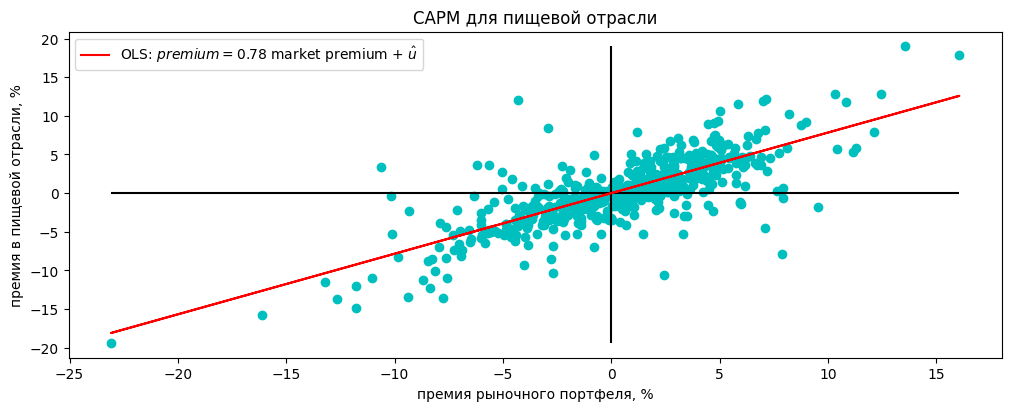
\includegraphics[width=0.8\linewidth]{capm_no_cost.png}
    \caption{CAPM модель, регрессия без константы}
    \label{fig:capm_nc}
\end{figure}

\textbf{Вариант, если модель CAPM не пройдена}

В качестве иллюстрации рассмотрим очень простую модель налогообложения, в которой будем для простоты игнорировать, что налоги могут считаться по прогрессивной шкале (так в целом было в России до 2025 года).

\[\text{taxes}_i = \beta_1 \times \text{income}_i + u_i\]

где $\text{taxes}_i$ — объём подоходных налогов, уплачиваемый каждым индивидом,
$\text{income}_i$ — налогооблагаемая база,
$\beta_1$ — ставка подоходного налога (для России до 2025 года ожидается, что при оценивании будет близка к 13\%).

Казалось бы, такая линейная регрессия без константы должна подойти для нашей задачи, ведь если доходов нет, то и подоходные налоги платить не надо. Значит, линия регрессии должна проходить через начало координат.

\item[3.] В модели парной регрессии с константой
\[
y_i = \beta_1 + \beta_2 x_i + u_i
\]
МНК-оценки для параметров $\beta_1$ и $\beta_2$ выглядят следующим образом:
\[
\hb_2 = \sum_{i=1}^n \frac{(x_i - \bar{x})(y_i - \bar{y})}{(x_i - \bar{x})^2}, \quad \hb_1 = \bar{y} - \hb_2 \bar{x}.
\]

\end{enumerate}

Результаты оценивания коэффициента $\hb_2$ можно проинтерпретировать аналогично предыдущей модели, 
производная прогноза по регрессору равна $\frac{\partial \hy_i}{\partial x_i} = \hb_2$. 
После интерпретации эффекта, который $x_i$ оказывает на $y_i$, можно заняться интерпретацией константы.
Оценка коэффициента $\hb_1$ — это прогноз $\hy_i$ при $x_i = 0$. 
Иногда оценка константы может иметь смысл. 
Давайте не поверим классической постановке модели и оценим модель CAPM с константой.
В этом случае линия регрессии не обязана проходить через точку $(0, 0)$ на графике.

Будем использовать те же самые обозначения для премии за риск для выбранных ценных бумаг и рыночной премии за риск:

\[
\text{premium}_i = \beta_1 + \beta_2 \times \text{market-premium}_i + u_i,
\]
где $\beta_2$ – мера систематического (рыночного) риска бумаги (портфеля).

\begin{figure}
    \centering
    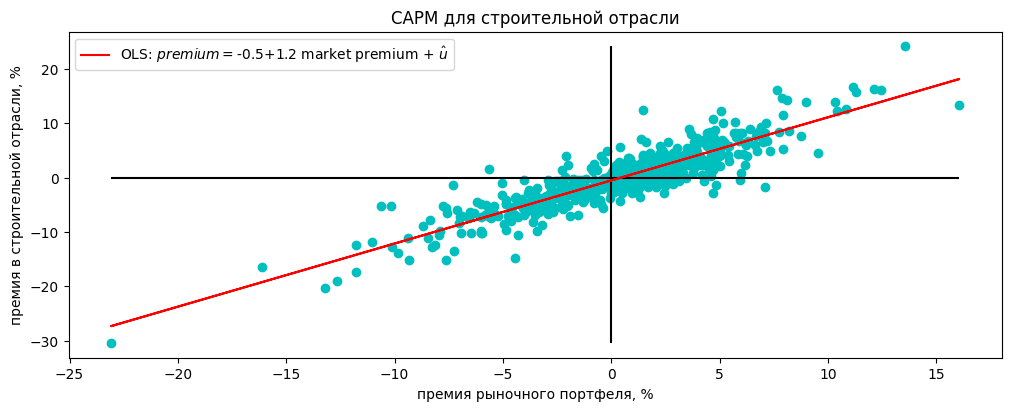
\includegraphics[width=0.8\linewidth]{capm_const.png}
    \caption{CAPM модель, регрессия с константой}
    \label{fig:cpam_c}
\end{figure}

\href{https://colab.research.google.com/drive/1ZQ7QuVCJS4I_GsXUrr7z7O-3wqXkXSMN?usp=sharing}{Оценённая} линия регрессии для строительной отрасли получилась следующая: 
\[
\text{premium}_i = -0.5 + 1.2 \times \text{market-premium}_i + \hu_i
\] 
Линия регрессии изображена на рисунке \ref{fig:cpam_c}. 
При росте премии за риск для рыночного портфеля на 1 пп премия в строительной отрасли растёт на 1.2 пп, что говорит о, видимо, более высоких рисках в строительной сфере, которые хозяева фирм пытаются компенсировать. Более того, у нас оценена константа $\hb_1 = -0.5$. 
Если бы доходность рыночного портфеля равнялась безрисковой ставке (рыночная премия за риск $\text{market-premium}_i = 0$), то премия за риск в строительной отрасли была бы $-0.5$. То есть, если бы рыночный портфель был безрисковым, то инвесторы уходили бы из строительного сектора.

На самом деле, константа не всегда осмысленна. 
Рассмотрим короткий пример зависимости длины остановочного пути\footnote{путь, пройденный за время реакции водителя и фактического торможения} от скорости автомобиля: 
\[
\text{dist}_i = \beta_1 + \beta_2 \times \text{speed}_i + u_i,
\]

\begin{figure}
    \centering
    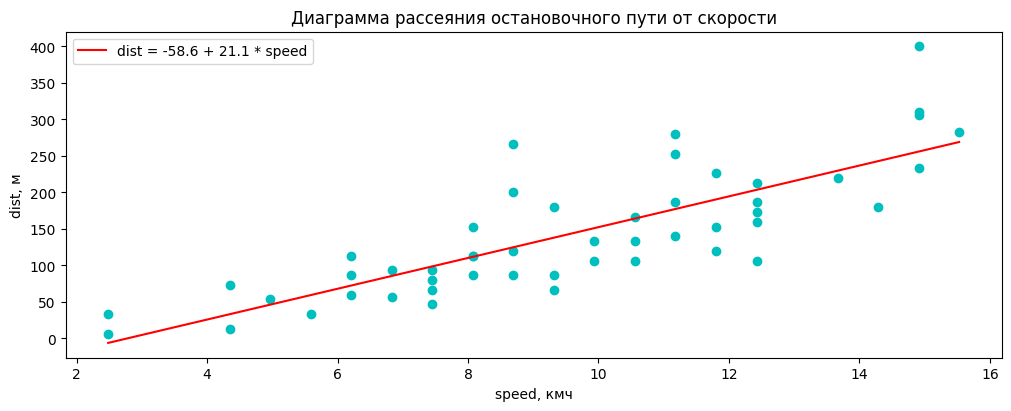
\includegraphics[width=0.8\linewidth]{cars_ds.png}
    \caption{Пример модели с константой, которая ничего не означает}
    \label{fig:cars}
\end{figure}

\href{https://colab.research.google.com/drive/1ZQ7QuVCJS4I_GsXUrr7z7O-3wqXkXSMN?usp=sharing}{Оценённая} модель (изображена на рисунке \ref{fig:cars}) получилась следующей: 
\[
\text{speed}_i = -58.6 + 21.1 \times \text{dist}_i + \hu_i.
\]
Коэффициенты показывают, что изменение скорости на один километр в час (ceteris paribus, при прочих равных факторах) приводит к росту остановочного пути на 21 метр. 
Если же скорость равна нулю, то не стоит говорить, что остановочный путь должен составить $-60$ метров.
В данном случае константа просто принимает значение параметра для наилучшего прохождения прямой через точки.

\subsection{Как я перестал беспокоиться и полюбил матричное дифференцирование}

Мы планируем перейти к рассмотрению регрессий с большим числом факторов, поэтому полезна будет матричная запись модели и, соответственно, матричное дифференцирование. 
Этому и будет посвящён данный раздел.

Много полезных фактов про матрицы можно найти в шикарной книжке «Поваренная книга любителя матриц» Петерсона и Педерсона \cite{petersen2012matrix}.


Нам чаще всего придётся дифференцировать скалярную функцию по векторному аргументу. 
По умолчанию вектор записывают столбцом и в большинстве источников производная по векторному аргументу тоже является столбцом,
\[
\frac{\partial r}{\partial s} = \grad r = \begin{pmatrix}
    \partial r/\partial s_1 \\
    \partial r/\partial s_2 \\
    \vdots \\
    \partial r/\partial s_k \\    
\end{pmatrix}
\]
Это сделано для того, чтобы размер результата дифференцирования совпадал с размером вектора $s$, по которому дифференцируют, и равнялся $[k \times 1]$. 
Например, для функции $f(x) = x_1^2 + x_2^3 + x_1 \cdot x_3^4$ векторная производная равна
\[
\frac{\partial f}{\partial x} = \grad f = \begin{pmatrix}
    2x_1 + x_3^4\\
    3x_2^2 \\
    4x_1 x_3^3 \\
\end{pmatrix}.
\]

Сформулируем основные правила дифференцирования скалярных выражений по векторному аргументу:
\[
\frac{\partial a^T s}{\partial s} = \frac{\partial s^T a}{\partial s} = \frac{\partial \sum s_i a_i}{\partial s} = a = \begin{pmatrix}
    a_1 \\
    a_2 \\
    \vdots \\
    a_n \\
\end{pmatrix}
\]
\[
\frac{\partial s^T A s}{\partial s} = \frac{\partial \sum_{ij}A_{ij}s_i s_j}{\partial s} = (A + A^T)s
\]
В частности, для суммы квадратов правило превращается в 
\[
\frac{\partial s^T s}{\partial s} = \frac{\partial \sum s_i^2}{\partial s}  = 2s = \begin{pmatrix}
    2s_1 \\
    2s_2 \\
    \vdots \\
    2s_n \\
\end{pmatrix}
\]


В более сложном случае дифференцирования вектора по вектору оказывается полезной матрица Якоби.
В ней строки отвечают за элементы дифференцируемой функции, а столбцы — за элементы вектора, по которому дифференцируют. 

\begin{definition}[матрица Якоби]
Для векторов $r$ размера $[n \times 1]$ и $s$ размера $[k \times 1]$ производной $\partial r/\partial s$ или матрицей Якоби называют матрицу, в которой дифференцируемые элементы записывают по строкам, а элементы, по которым берут производную, — по столбцам:
    \[
    J = \frac{\partial r}{\partial s} = \begin{pmatrix}
        \partial r_1/\partial s_1 & \partial r_1/\partial s_1 & \dots & \partial r_1/\partial s_n \\
        \partial r_2/\partial s_1 & \partial r_2/\partial s_1 & \dots & \partial r_2/\partial s_n \\
        \vdots & & & \vdots \\
        \partial r_n/\partial s_1 & \partial r_n/\partial s_1 & \dots & \partial r_n/\partial s_n \\   
    \end{pmatrix}.
    \]
\end{definition}

Например, для функции $f(x) = \begin{pmatrix}
    x_1 + 3x_2 \\
    x_1 \cdot x_2^2  \\
\end{pmatrix}$ матрица Якоби равна
\[
J = \frac{\partial f}{\partial x} = \begin{pmatrix}
    1 & 3 \\
    x_2^2 & 2x_1 x_2 \\
\end{pmatrix}.
\]


Будьте бдительны! 
Обозначение для матрицы Якоби часто используют ровно то же, что для производной скалярной функции по векторному аргументу, $\partial r/\partial s$. 
При этом для скалярной функции $r$ матрица Якоби «положит» все производные в строчку, а производная скалярной функции по векторному аргументу положит те же производные в столбик.
\[
J = (\partial r/\partial s_1, \dots, \partial r/\partial s_n) \quad \frac{\partial r}{\partial s} = \begin{pmatrix}
    \partial r/\partial s_1 \\
    \dots \\
    \partial r/\partial s_n \\
\end{pmatrix}
\]

Избежать этой путаницы с упаковкой производных то в строчку, то в столбец позволяет дифференциал. 
У дифференциала всегда-всегда размерность совпадает с размерностью исходного дифференцируемого объекта.

Например, для функции $f(x) = \begin{pmatrix}
    x_1 + 3x_2 \\
    x_1 \cdot x_2^2  \\
\end{pmatrix}$ дифференциал равен
\[
df = \begin{pmatrix}
    dx_1 +  3  dx_2 \\
    x_2^2 dx_1 +  2x_1 x_2 dx_2 \\
\end{pmatrix}.
\]

Если брать дифференциал скалярной функции $s$ по векторному аргументу $r$, то он примет вид
\[
ds = (\partial s/\partial r)^T dr = \grad^T s dr,
\]
поэтому из дифференциала легко извлечь градиент. 

Например, если в результате долгих вычислений оказалось, что $ds =  2r^T dr$,
то мы легко можем извлечь градиент-столбец $\grad s = 2r$.

Напишем и правила для работы с дифференциалом.
Здесь $A$, $B$ — постоянные матрицы; $a$, $b$ — постоянные векторы; $R$, $S$ — матрицы переменных; $r$, $s$ — векторы переменных.

Дифференциал постоянной матрицы равен нулю:
\[
dA = 0.
\]
При взятии дифференциала произведения важно  сохранять порядок матриц $R$ и $S$:
\[
d(RS) = dR \cdot S + R \cdot dS.
\]
В частности,
\[
d(ARB) = A \cdot dR \cdot B.
\]
Для суммы квадратов правило превращается в 
\[
d s^T s = d(\sum s_i^2) = 2s^T ds = 2 \sum s_i ds_i.
\]
Линейность сохраняется для следа матрицы
\[
d \trace R = \trace dR.
\]


\subsection{Матричное представление регрессии}
Пусть теперь в модель для $y$ включены $k$ регрессоров $x_1, x_2, \dots x_k$. 
Если в модель регрессии включена константа, то мы считаем, что $x_{i1}=1$ для всех $i=1, \dots, n$.
Модель вида
\[
y_i = \beta_1 x_{i1} + \beta_2 x_{i2} + \dots + \beta_k x_{ik} + u_i
\]
назовём моделью множественной регрессии.

Вектор зависимой переменной $y$ имеет размер $[n \times 1]$, матрица признаков $X$ —  $[n \times k]$, вектор параметров модели $\beta$ — $[k \times 1]$, вектор случайной ошибки $u$ — $[n \times 1]$:

\[
y =  \begin{pmatrix}
y_1 \\
y_2 \\
\dots \\
y_n
 \end{pmatrix},\quad
X = \begin{pmatrix}
    x_{11} & \dots & x_{1k} \\
    x_{21} & \dots & x_{2k} \\
    \vdots &   & \vdots \\
    x_{n1} & \dots & x_{nk} \\
\end{pmatrix}, \quad
\beta = \begin{pmatrix}
    \beta_1\\
    \beta_2\\
    \dots \\
    \beta_k
\end{pmatrix}, \quad
u =  \begin{pmatrix}
u_1 \\
u_2 \\
\dots \\
u_n
 \end{pmatrix}.
\]

Используя введённые обозначения модель множественной регрессии
\[
y_i = \beta_1 x_{i1} + \beta_2 x_{i2} + \dots + \beta_k x_{ik} + u_i
\]
можно переписать в матричном виде
\[
y = X\beta + u.
\]

Для наглядности можно преобразовать упражнение для парной линейной регрессии с константой из раздела \ref{sec:optimization} в матричный вид. Если при наличии в модели константы $x_{i1} = 1$ для всех $i$ и $(x_{12}, y_1) = (1, 1);$ $(x_{22}, y_2) = (1, 2);$ $(x_{32}, y_3) = (0, 3);$ $(x_{42}, y_4) = (0, 4)$: 
\[
y = \begin{pmatrix}
    1 \\
    2 \\
    3 \\
    4 \\
\end{pmatrix}, \quad 
X = \begin{pmatrix}
    1 & 1 \\
    1 & 1 \\
    1 & 0 \\
    1 & 0 \\
\end{pmatrix}.
\]

\subsection{Решение оптимизационной задачи МНК с матрицами}


Для матричную регрессионной модели
\[
y = X\beta + u
\]
оптимизационную задачу МНК можно переписать как
\[
Q(\hb) = (y-X\hb)^T(y-X\hb) = \hu^T\hu \to \underset{\hb}{\min}.
\]

Найдём МНК-оценку вектора $\beta$, используя матричное дифференцирование.

Запишем необходимое условие для задачи минимизации: 
\[
\frac{\partial Q(\hb)}{\partial \hb} = -2X^{T}y + 2X^TX\hb = 0
\]
\[
2X^TX\hb = 2X^{T}y
\]
Если матрица $X^TX$ размера $[k\times k]$ обратима, то формула для оценок принимает вид
\[
\hb_{\ols} = (X^TX)^{-1}X^Ty.
\]
Если матрица $X^TX$ не обратима, то оценки МНК будут неединственными. 
Подобная проблемная ситуация возникает, если среди столбцов матрицы $X$ есть линейно-зависимые, и называется \emph{строгой мультиколлинеарностью}.

Для проверки достаточных условий второго порядка найдём матрицу Гессе в точке оптимума
\[
\frac{\partial^2 Q(\hb)}{\partial \hb \partial \hb^T} = 2X^TX.
\]
Если матрица $X^TX$ обратима, то она положительно определена и $\hb_{\ols}$ —  точка глобального минимума. 


Для полноты изложения найдём условие первого порядка для оптимального $\hb$ и матрицу Гессе альтернативным способом — через дифференциал.

Запишем дифференциал для функции $Q(\hb)$ и выделим внутри него градиент,
\[
dQ(\hb) = 2(X\hb - y)^TX d\hb = (\grad Q(\hb))^T d\hb.
\]
Приравняем градиент к нулю
\[
\grad Q(\hb) =  2X^T(X\hb - y) = 0,
\]
и получим прежнее условие первого порядка:
\[
2X^TX\hb = 2X^{T}y
\]
Матрицу Гессе можно выделить внутри второго дифференциала,
\[
d^2 Q = d(2(X\hb - y)^TX d\hb) = d\hb^T \cdot 2X^T X \cdot d\hb. 
\]
Как и ранее, матрица Гессе равна $\frac{\partial^2 Q(\hb)}{\partial \hb \partial \hb^T} = 2X^TX$.

Полученную оценку $\hb = (X^TX)^{-1}X^Ty$ называют МНК-оценкой $\hb_{\ols}$. 
Далее в целях снижения занудства мы иногда будем опускать нижний индекс $\ols$ и писать $\hb$ вместо $\hb_{\ols}$.

Для нашего примера с 
\[
y = \begin{pmatrix}
    1 \\
    2 \\
    3 \\
    4 \\
\end{pmatrix}, \quad 
X = \begin{pmatrix}
    1 & 1 \\
    1 & 1 \\
    1 & 0 \\
    1 & 0 \\
\end{pmatrix}
\]

\[ X^TX = \begin{pmatrix}
    1 & 1 & 1 & 1\\
    1 & 1 & 0 & 0\\
\end{pmatrix}
\begin{pmatrix}
    1 & 1 \\
    1 & 1 \\
    1 & 0 \\
    1 & 0 \\
\end{pmatrix} =
\begin{pmatrix}
    4 & 2 \\
    2 & 2 \\
\end{pmatrix},
(X^TX)^{-1} = 
\begin{pmatrix}
    0.5 & -0.5 \\
    -0.5 & 1 \\
\end{pmatrix},
X^Ty = 
\begin{pmatrix}
    10 \\
    3\\
\end{pmatrix}.
\]

\[
\hb = \begin{pmatrix}
    0.5 & -0.5 \\
    -0.5 & 1 \\
\end{pmatrix}
\begin{pmatrix}
    10 \\
    3\\
\end{pmatrix} = 
\begin{pmatrix}
    3.5 \\
    -2\\
\end{pmatrix}.
\]

Убедитесь, что результаты совпадают с примером в разделе \ref{sec:optimization}.

\subsection{Геометрия МНК}

Кучу интересных геометрических фактов можно найти в статье \cite{gnilova2018gauss} «Как встретились Гаусс, Марков и Пифагор?»

Метод наименьших квадратов имеет шикарную геометрическую интерпретацию.
Геометрия позволяет не только вывести оценки, но и легко увидеть некоторые их свойства. 

Для удобства рассмотрим случай двух регрессоров с константой
\[
\hy_i = \hb_1 + \hb_2 a_i + \hb_3 b_i.
\]
Обозначим вектор из сплошных единиц буквой $\one$, $\one = \begin{pmatrix}
    1 \\
    1 \\
    \vdots \\
    1
\end{pmatrix}$.
Буква $\one$ не является стандартным обозначением для вектора из единиц 
и намекает на строевой лес, «ship forest».
Также отметим, что вектор $\one$ нельзя называть единичным, единичный вектор — это вектор из нулей, в котором есть ровно одна единице. 

С помощью вектора из единиц мы можем записать вектор прогнозов $\hy$ в виде
\[
\hy = \hb_1 \one + \hb_2 a + \hb_3 b.
\]
Вектор $\hy$ — это линейная комбинация векторов $\one$, $a$ и $b$,
$\hy \in \Span(\one, a, b)$. 
Под $\Span(s, a, b)$ мы обозначаем линейную оболочку векторов.
Для наглядности можно представлять себе конкретный пример, 
\[
y = \begin{pmatrix}
    2 \\
    2 \\
    3 \\
    4 \\
\end{pmatrix}, \quad 
X = \begin{pmatrix}
    \vertbar & \vertbar & \vertbar \\
    s & a & b \\
    \vertbar & \vertbar & \vertbar \\    
\end{pmatrix} = \begin{pmatrix}
    1 & 1 & 1 \\
    1 & 1 & 2 \\
    1 & 0 & 3 \\
    1 & 0 & 4 \\
\end{pmatrix}
\]

Теперь вспомним целевую функцию метода наименьших квадратов
\[
\sum_{i=1}^n (y_i - \hy_i)^2 \to \min_{\hb_1, \hb_2, \hb_3}.
\]
Величина $\sum_{i=1}^n (y_i - \hy_i)^2$ — это квадрат длины вектора $y - \hy$, то есть $\sum_{i=1}^n (y_i - \hy_i)^2 = \norm{y - \hy}^2$.

И теперь мы можем сформулировать метод наименьших квадратов геометрически!
\begin{explanation}
    Метод наименьших квадратов ищет вектор прогнозов $\hy$ внутри линейной оболочки регрессоров $\Span(s, a, b)$ поближе к вектору  зависимой переменной $y$.
\end{explanation}

Конечно же, оптимальным решением оказывается проекция вектора $y$ на линейную оболочку $\Span(s, a, b)$.

\tdplotsetmaincoords{40}{120}
\begin{tikzpicture}[tdplot_main_coords]

\coordinate (O) at (0,0,0);
\coordinate (haty) at (-0.9,3);
\coordinate (s) at (-1.3,1.2);
\coordinate (a) at (1,-2);
\coordinate (b) at (1, 1.4);

\tdplotsetcoord{S}{10}{35}{0}  % икс
\tdplotsetcoord{P}{7}{30}{90} % игрек

\draw[->] (O) -- (P) node[anchor=north west]{$y$};
\draw (0,0.5) ellipse (4.5cm and 1cm) node[anchor=north, below=1cm]{\footnotesize$\Span(s, a, b)$};

\draw[->] (O) -- (haty) node[anchor=north east]{\small $\hat y$};
\draw[->] (O) -- (a) node[anchor=north east]{\small $a$};
\draw[->] (O) -- (b) node[anchor=south west]{\small $b$};
\draw[->] (O) -- (s) node[anchor=north west]{\small $\one$};
\draw[dashed, <-] (P) -- (haty) node[above=1.5cm, xshift=0.3cm]{\small $\hat u$};

\tkzMarkRightAngle[size=0.15](P,haty,O);

\end{tikzpicture}

В случае произвольной матрицы $X$ место линейной оболочки $\Span(s, a, b)$ 
займёт линейная оболочка всех столбцов матрицы $X$, $\Span(\col_1 X, \col_2 X, \dots, \col_k X)$, которую мы для краткости будем обозначать $\colspan(X)$.

Условием первого порядка будет ортогональность вектора остатков $\hu = y - \hy$ каждому из регрессоров,
\[
\hu \perp \Span(s, a, b) \quad \Leftrightarrow \quad \begin{cases}
    \hu \perp s \\
    \hu \perp a \\
    \hu \perp b
\end{cases}.
\]
Поскольку оптимальный вектор прогнозов $\hy$ лежит в линейной оболочке $\Span(s, a, b)$, то вектор остатков $\hu$ перпендикулярен и ему тоже, $\hu \perp \hy$.

Условие ортогональности векторов означает, что скалярное произведение равно нулю, поэтому
\[
\begin{pmatrix}
    \horzbar s^T \horzbar \\
    \horzbar a^T \horzbar \\
    \horzbar b^T \horzbar \\
\end{pmatrix} \cdot \hu = 0 \quad \Leftrightarrow \quad X^T \hu = 0.
\]

А далее из условия ортогональности регрессоров и остатков $X^T \hu = 0$ можно получить и явно формулы оценок всех коэффициентов.
Подставим формулу для прогнозов, $\hy = X\hb$, и решим полученное уравнение $X^T (y - X\hb) = 0$.
Раскрываем скобки,
\[
X^T y - X^T X\hb = 0 \quad \Leftrightarrow \quad X^TX \hb = X^T y.
\]
Для рассматриваемого игрушечного примера,
\[
X^TX = \begin{pmatrix}
    1 & 1 & 1 & 1 \\
    1 & 1 & 0 & 0 \\
    1 & 2 & 3 & 4\\
\end{pmatrix}
\begin{pmatrix}
    1 & 1 & 1 \\
    1 & 1 & 2 \\
    1 & 0 & 3 \\
    1 & 0 & 4 \\
\end{pmatrix} = 
\begin{pmatrix}
    4 & 2 & 10 \\
    2 & 2 & 3 \\
    10 & 3 & 30 \\
\end{pmatrix}, \quad 
\]

\[
X^Ty = \begin{pmatrix}
    1 & 1 & 1 & 1 \\
    1 & 1 & 0 & 0 \\
    1 & 2 & 3 & 4\\
\end{pmatrix}
\begin{pmatrix}
    2 \\
    2 \\
    3 \\
    4 \\
\end{pmatrix}=
\begin{pmatrix}
    11 \\
    4 \\
    31 \\
\end{pmatrix},
\]

Если нам повезло, и матрица $X^TX$ обратимая, то 
\[
\hb = (X^TX)^{-1} X^Ty.
\]

На нашем примере $\hb = \begin{pmatrix}
    4 & 2 & 10 \\
    2 & 2 & 3 \\
    10 & 3 & 30 \\
\end{pmatrix}^{-1}
\begin{pmatrix}
    11 \\
    4 \\
    31 \\
\end{pmatrix}= 
\begin{pmatrix}
    12.75 & -7.5 & -3.5 \\
    -7.5 & 5 & 2 \\
    -3.5 & 2 & 1 \\
\end{pmatrix}
\begin{pmatrix}
    11 \\
    4 \\
    31 \\
\end{pmatrix} =
\begin{pmatrix}
    1.75 \\
    -0.5\\
    0.5 \\
\end{pmatrix} 
$

Заметим, что просто сократить матрицу $X^T$ слева и справа нельзя потому, что она точно не обратимая! 
Матрица $X^T$ имеет размер $[k \times n]$ и не является квадратной.

Готовая формула для вектора прогнозов равна 
\[
\hy = X\hb = X(X^TX)^{-1} X^Ty.
\]

На нашем примере $\hy = \begin{pmatrix}
    1 & 1 & 1 \\
    1 & 1 & 2 \\
    1 & 0 & 3 \\
    1 & 0 & 4 \\
\end{pmatrix}
\begin{pmatrix}
    1.75 \\
    -0.5\\
    0.5 \\
\end{pmatrix} = 
\begin{pmatrix}
    1.75 \\
    2.25 \\
    3.25 \\
    3.75 \\
\end{pmatrix}.
$


\begin{definition}[матрица-шляпница]
Матрица $X(X^TX)^{-1} X^T$ часто обозначается буквой $H$ и неформально называется \emph{матрицей-шляпницей} (hat matrix).
Она «надевает» на $y$ шляпку, $Hy = \hat y$.
Формально матрица $H$ также называется матрицей-проектором. 
Она проецирует любой вектор на линейную оболочку всех регрессоров $\Span(\col_1 X, \col_2 X, \dots, \col_k X)$.
\end{definition}

На нашем примере $H = \begin{pmatrix}
    0.75 & 0.25 & 0.25 & -0.25\\
    0.25 & 0.75 & -0.25 & 0.25\\
    0.25 & -0.25 & 0.75 & 0.25\\
    -0.25 & 0.25 & 0.25 & 0.75\\
\end{pmatrix}.$
Заметим, что матрица-шляпница $H$ имеет размер $[n \times n]$.


Вектор $\hb$ состоит из $k$ оценок $\hb_1$, $\hb_2$, \dots, $\hb_k$, поэтому его напрямую невозможно нарисовать в пространстве $\RR^n$.
Однако, оказывается, что веса, с которыми компоненты вектора зависимой переменной входят в каждую из оценок, можно изобразить!
Заметим, что вектор оценок можно записать в виде
\[
\hb = (X^TX)^{-1} X^Ty = W^T y, \text{ где } W= X(X^TX)^{-1}.
\]
\[
\hb = \begin{pmatrix}
    \hb_1 \\
    \hb_a \\
    \hb_b \\
\end{pmatrix}= \begin{pmatrix}
    \horzbar & w_1^T & \horzbar \\
    \horzbar & w_2^T & \horzbar \\
    \horzbar & w_3^T & \horzbar \\    
\end{pmatrix} \cdot \begin{pmatrix}
    \vertbar \\
    y \\
    \vertbar
\end{pmatrix} = 
\begin{pmatrix}
    \vertbar & \vertbar & \vertbar \\
    w_1 & w_2 & w_3 \\
    \vertbar & \vertbar & \vertbar \\    
\end{pmatrix}^T\cdot \begin{pmatrix}
    \vertbar \\
    y \\
    \vertbar
\end{pmatrix} = \begin{pmatrix}
1.75 & -0.5 & -0.5 \\ 
-1.75 & 1.5 & 0.5 \\
2.25 & -1.5 & -0.5 \\
-1.25 & 0.5 & 0.5 \\
\end{pmatrix}^T\cdot \begin{pmatrix}
    \vertbar \\
    y \\
    \vertbar
\end{pmatrix}.
\]
То есть, каждая оценка $\hb_j$ — это взвешенные наблюдения зависимой переменной $y_1$, $y_2$, \dots, $y_n$.
Например, оценка первого коэффициента $\hb_1$ — это скалярное произведение первого столбца $W$ и зависимой переменной $y$,
\[
\hb_1 = \scalp{\row_1 W^T, y} = \scalp{\col_1 W, y} = \scalp{w_1, y}  = w_{11}y_1 + w_{21} y_2 + \dots + w_{n1} y_n 
\]
В нашем частном случае четырёх наблюдений,
\[
\hb_1 = 1.75 y_1 - 1.75 y_2 + 2.25y_3 - 1.25 y_4.
\]
Обратим внимание на запись $W = X(X^TX)^{-1}$.
Для столбца весов $w_1$ она означает, что
\[
\begin{pmatrix}
    \vertbar \\
    w_1 \\
    \vertbar
\end{pmatrix} =
\begin{pmatrix}
    1.75 \\
    -1.75 \\
    2.25 \\
    -1.25
\end{pmatrix} =
\begin{pmatrix}
    \vertbar & \vertbar & \vertbar \\
    s & a & b \\
    \vertbar & \vertbar & \vertbar \\    
\end{pmatrix} \cdot \col_1 (X^TX)^{-1} = 
\begin{pmatrix}
    \vertbar & \vertbar & \vertbar \\
    s & a & b \\
    \vertbar & \vertbar & \vertbar \\    
\end{pmatrix} \cdot \begin{pmatrix}
    12.75 \\
    -7.5 \\
    -3.5 \\
\end{pmatrix}
\]
То есть, вектор весов $\col_1 W$ лежит в линейной оболочке регрессоров, $\col_1 W \in  \colspan X$.
Например, при проецировании каждого столбца матрицы $W$ на линейную оболочку регрессоров ничего не происходит, $HW = W$.

% TODO: хотим красивую картинку вместо handmade :)
\begin{minipage}{\textwidth}
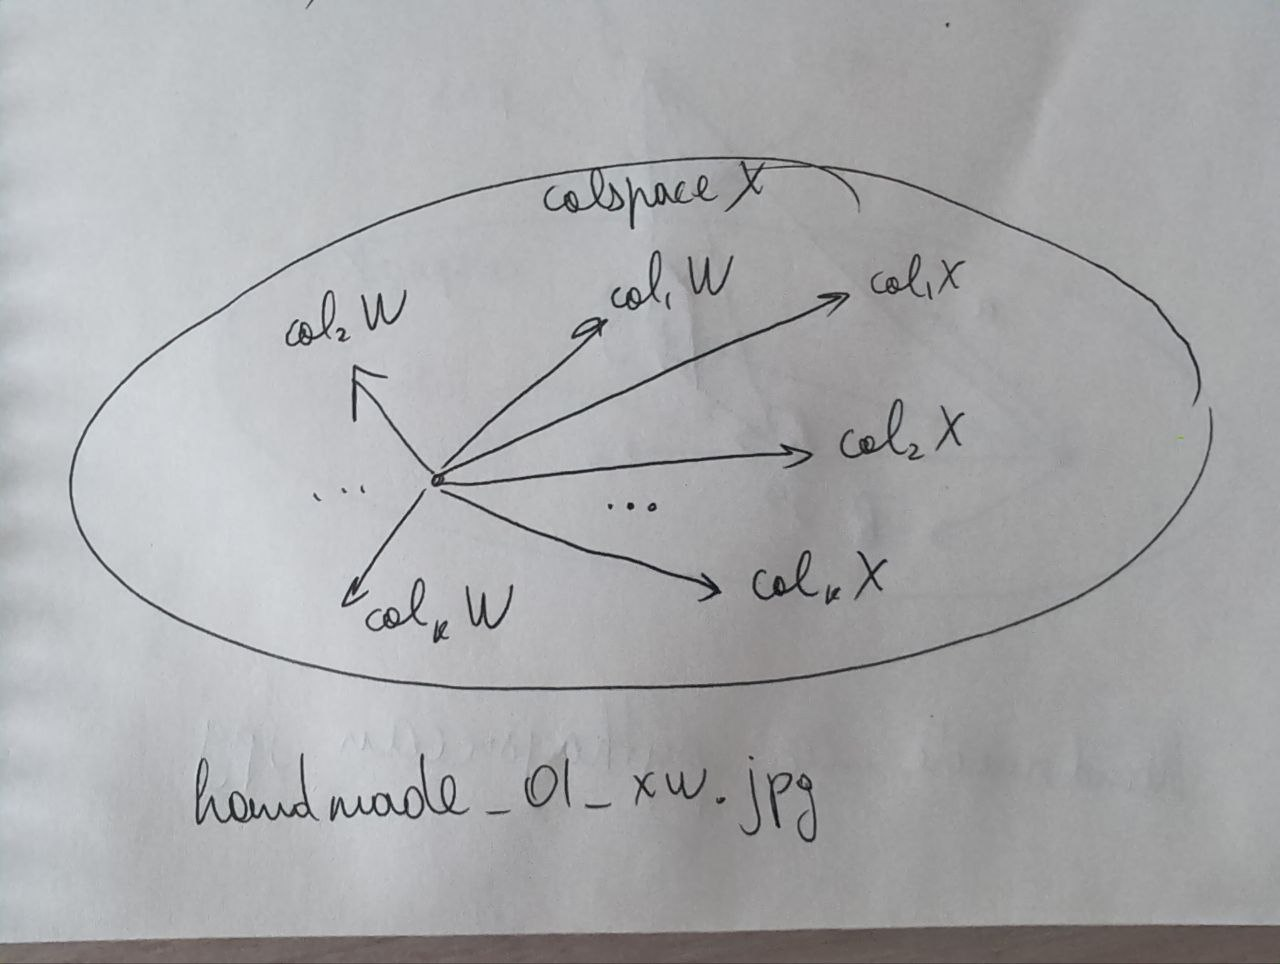
\includegraphics[width=7cm]{handmade/handmade_01_xw.jpg}
\end{minipage}


% TODO: поправить подписи векторов на картинке
%\tdplotsetmaincoords{40}{120}
%\begin{tikzpicture}[tdplot_main_coords]

%\coordinate (O) at (0,0,0);
%\coordinate (x1) at (-1.3,1.2);
%\coordinate (x2) at (1,-2);
%\coordinate (x3) at (1, 1.4);
%\coordinate (w1) at (-1,1.2);
%\coordinate (w2) at (1.2,-2.1);
%\coordinate (w3) at (1.2, 1.4);


%\tdplotsetcoord{S}{10}{35}{0}  % икс
%\tdplotsetcoord{P}{7}{30}{90} % игрек

%\draw (0,0.5) ellipse (6cm and 1.5cm) node[anchor=north, below=2cm]{\footnotesize$\Span(\col_1 X, \col_2 X, \dots)$};

%\draw[->] (O) -- (x1) node[anchor=north east]{\small $x_1$};
%\draw[->] (O) -- (x2) node[anchor=north east]{\small $x_2$};
%\draw[->] (O) -- (x3) node[anchor=south west]{\small $x_3$};
%\draw[->] (O) -- (w1) node[anchor=north east]{\small $w_1$};
%\draw[->] (O) -- (w2) node[anchor=north east]{\small $w_2$};
%\draw[->] (O) -- (w3) node[anchor=south west]{\small $w_3$};

%\end{tikzpicture}

В этом равенстве можно убедиться и средствами линейной алгебры,
\[
HW = X(X^TX)^{-1} X^T X(X^TX)^{-1} = X(X^TX)^{-1} = W.
\]

\subsection{Показатели качества подгонки модели}

После оценивания регрессионной модели полезно проанализировать, насколько она «хороша». 
А именно, насколько похожи прогнозы $\hy_i$ на исходные наблюдения $y_i$.
Для этого нужен показатель качества подгонки модели.

Назовём общей суммой квадратов ($\TSS$) величину $\sum_{i=1}^n (y_i - \bar{y})^2$. 
Рассмотрим её разложение в сумму
\[
\sum_{i=1}^n (y_i - \bar{y})^2 = \sum_{i=1}^n (y_i - \hy_i)^2 + 2\sum_{i=1}^n (y_i - \hy_i)(\hy_i - \bar{y}) + \sum_{i=1}^n (\hy_i - \bar{y})^2.
\]
Покажем, что $\sum_{i=1}^n (y_i - \hy_i)(\hy_i - \bar{y}) = 0$:

\[
\sum_{i=1}^n (y_i - \hat{y}_i)(\hat{y}_i - \bar{y}) = \sum_{i=1}^n (y_i - \hat{y}_i)\hat{y}_i - \bar{y}\sum_{i=1}^n (y_i - \hat{y}_i) \\
= \sum_{i=1}^n (y_i - \hat{y}_i)\hat{y}_i - 0 \quad =
\]
\[
= \sum_{i=1}^n (y_i - \hat{y}_i)(\hb_1 + \hb_2 x_{i2}+ \dots + \hb_k x_{ik} )
= \hb_1 \sum_{i=1}^n (y_i - \hat{y}_i) + \hb_2 \sum_{i=1}^n (y_i - \hat{y}_i)x_i + \dots + \hb_k \sum_{i=1}^n (y_i - \hat{y}_i)x_i = 0,
\]

Здесь мы пользовались двумя фактами:
\begin{enumerate}
    \item[1.] сумма остатков равна нулю $\sum_{i=1}^n (y_i - \hat{y}_i) = \sum_{i=1}^n \hu_i = 0$;
    \item[2.] $\sum_{i=1}^n (y_i - \hat{y}_i)x_{ij} = 0$ для всех $j=1,\dots,k$, так как остатки $\hu_i = (y_i - \hy_i)$ ортогональны регрессорам $x_j, j=1,\dots, k$.
\end{enumerate}

Заметим, что второе условие всегда выполнено, если используется метод наименьших квадратов. 
Первое условие будет гарантированно выполнено, если среди регрессоров будет присутствовать константа. 

Таким образом, получаем разложение
\[
\TSS = \sum_{i=1}^n (y_i - \bar{y})^2 = \sum_{i=1}^n (y_i - \hy_i)^2 + \sum_{i=1}^n (\hy_i - \bar{y})^2.
\]

Три составляющих этого разложения будут нам часто встречаться,

    \begin{tabular}{ccc}
    \toprule
        $\TSS = \sum_{i=1}^n (y_i - \bar{y})^2$ & Общая сумма квадратов &  Total Sum of Squares   \\
        $\ESS = \sum_{i=1}^n (\hy_i - \bar{y})^2$ & Объяснённая сумма квадратов & Explained sum of squares  \\
        $\RSS = \sum_{i=1}^n (y_i - \hy_i)^2$ & Сумма квадратов остатков & Residual sum of squares  \\
    \bottomrule
    \label{tab:sum_of_squares}
    \end{tabular}

Давайте для нашего примера рассчитаем все три показателя. Имеем:
\[
y = \begin{pmatrix}
    2 \\
    2 \\
    3 \\
    4 \\
\end{pmatrix}, \quad \hy = \begin{pmatrix}
    1.75 \\
    2.25 \\
    3.25 \\
    3.75 \\
\end{pmatrix}, \quad \bar{y} = 2.75.
\]

Тогда
\[
\TSS = \sum_{i=1}^n (y_i - \bar{y})^2 = (2-2.75)^2 + (2-2.75)^2 + (3-2.75)^2 + (4-2.75)^2 = 2.75,
\]
\[
\ESS = \sum_{i=1}^n (y_i - \bar{y})^2 = (1.75-2.75)^2 + (2.25-2.75)^2 + (3.25-2.75)^2 + (3.75-2.75)^2 = 2.5,
\]
\[
\RSS = \sum_{i=1}^n (y_i - \hy_i)^2 = (2-1.75)^2 + (2-2.25)^2 + (3-3.25)^2 + (4-3.75)^2 = 0.25.
\]
Нетрудно убедиться, что выполняется тождество $\TSS = \ESS + \RSS$.

Будьте бдительны! 
Некоторые источники используют иные обозначения. 
По поводу $\TSS$ разногласий в литературе не возникает. 
Под $\RSS$ иногда понимают регрессионную сумму квадратов, regression sum of squares, то есть $\ESS$ в нашем курсе. 
Под $\ESS$ некоторые авторы подразумевают сумму квадратов остатков, error sum of squares, то есть наш $\RSS$. 
Эта разница может быть критичной, например, при использовании формул из интернета, которые будут говорить противоположные нашему курсу вещи.

Запишем итоговую теорему.
\begin{theorem}
Если среди регрессоров присутствует константа, то
\[
\label{tss}
    \TSS = \ESS + \RSS.
\]
\end{theorem}


На картинке это равенство окажется школьной теоремой Пифагора:

% TODO: хотим красивую картинку вместо handmade :)
\begin{minipage}{\textwidth}
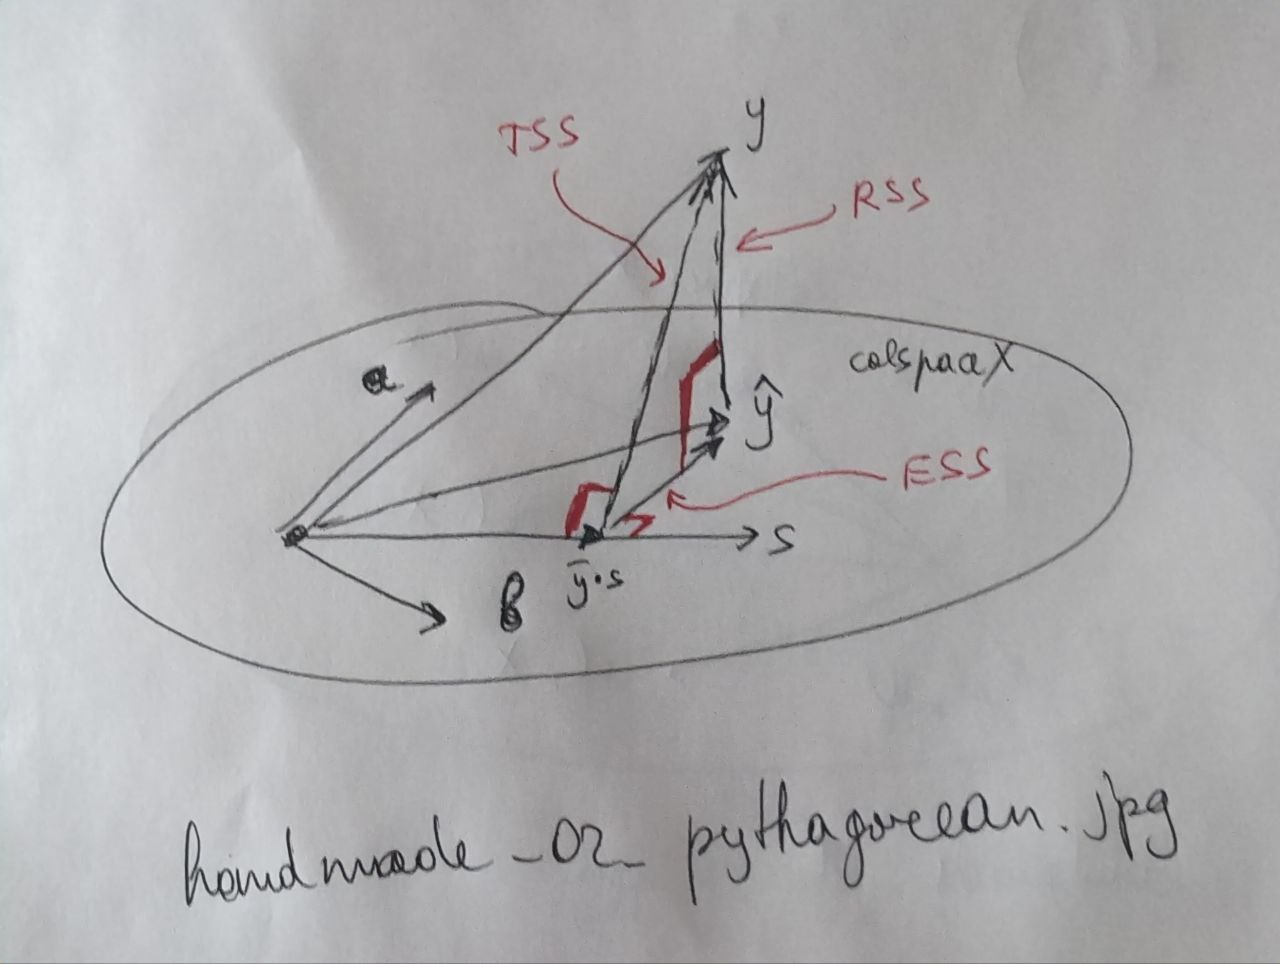
\includegraphics[width=7cm]{handmade/handmade_02_pythagorean.jpg}
\end{minipage}


И в самом деле, $\TSS = \sum (y_i - \bar y)^2 = \norm{y - \bar y\cdot s}^2$ — это квадрат длины гипотенузы $y - \bar y \cdot s$.
Длина катета $y - \hat y$ в квадрате даёт $\RSS = \sum(y_i - \hy_i)^2 = \norm{y - \hy}^2$.
Длина катета $\hy - \bar y s$ в квадрате даёт $\ESS = \sum(\hy_i - \bar y)^2 = \norm{\hy - \bar y \cdot s}^2$.
Напомним, что $s$ — это вектор строевого леса из единиц,
а треугольник является прямоугольным в силу того, что мы проецируем вектор $y$ на пространство $\colspan X$.




\begin{definition}[коэффициент детерминации]
Коэффициентом детерминации называется статистика 
\[
R^2 = \frac{\ESS}{\TSS} = 1 - \frac{\RSS}{\TSS}.
\]    
\end{definition}

При наличии константы в модели коэффициент детерминации $R^2 \in [0,1]$ и показывает, какая доля разброса зависимой переменной относительно её среднего объясняется регрессионной моделью.

В нашем примере коэффициент детерминации равен
\[
R^2 = \frac{\ESS}{\TSS} = \frac{2.5}{2.75} = 0.91.
\]
Так как в нашем примере константа включена в число регрессоров, мы можем проинтерпретировать этот результат следующим образом: доля разброса зависимой переменной $y$ относительно её среднего, объяснённая регерессионной моделью, составляет 0.91.

Ниже приведём альтернативное определение коэффициента детерминации.

\begin{definition}[коэффициент детерминации] В модели множественной регрессии с константой коэффициент детерминации $R^2$ — это квадрат выборочной корреляции между фактическими значениями зависимой переменной $y$ и предсказанными значениями $\hat{y}$, полученными по модели, 
\[
R^2 = \sCorr^2(y, \hy).
\]
\end{definition}

При отсутствии константы в модели нарушается равенство $\TSS = \ESS + \RSS$, в этом случае три формулы формулы $R^2 = \ESS/\TSS$, $R^2 = 1 - \RSS/\TSS$ и 
$R^2 = \sCorr^2(y, \hy)$ дают разные результаты.

В регрессии без константы, в зависимости от используемой формулы, софт может выдать даже отрицательное значение $R^2$.
В разные пакеты могут быть встроены разные формулы для подсчёта $R^2$ без константы, например, в \sklearn всегда используется формула $R^2 = 1 - \RSS/\TSS$, поэтому значения могут быть отрицательными. В \statsmodels при отсутствии константы формула меняется: $R^2 = 1 - \RSS/\sum_{i=1}^n y_i^2$ и значение всегда положительно.  
% TODO: check!

На картинке $R^2$ окажется квадратом косинуса угла $\phi$, $R^2 = \frac{ESS}{TSS} = \cos^2 \phi$.

% TODO: хотим красивую картинку вместо handmade :)
\begin{minipage}{\textwidth}
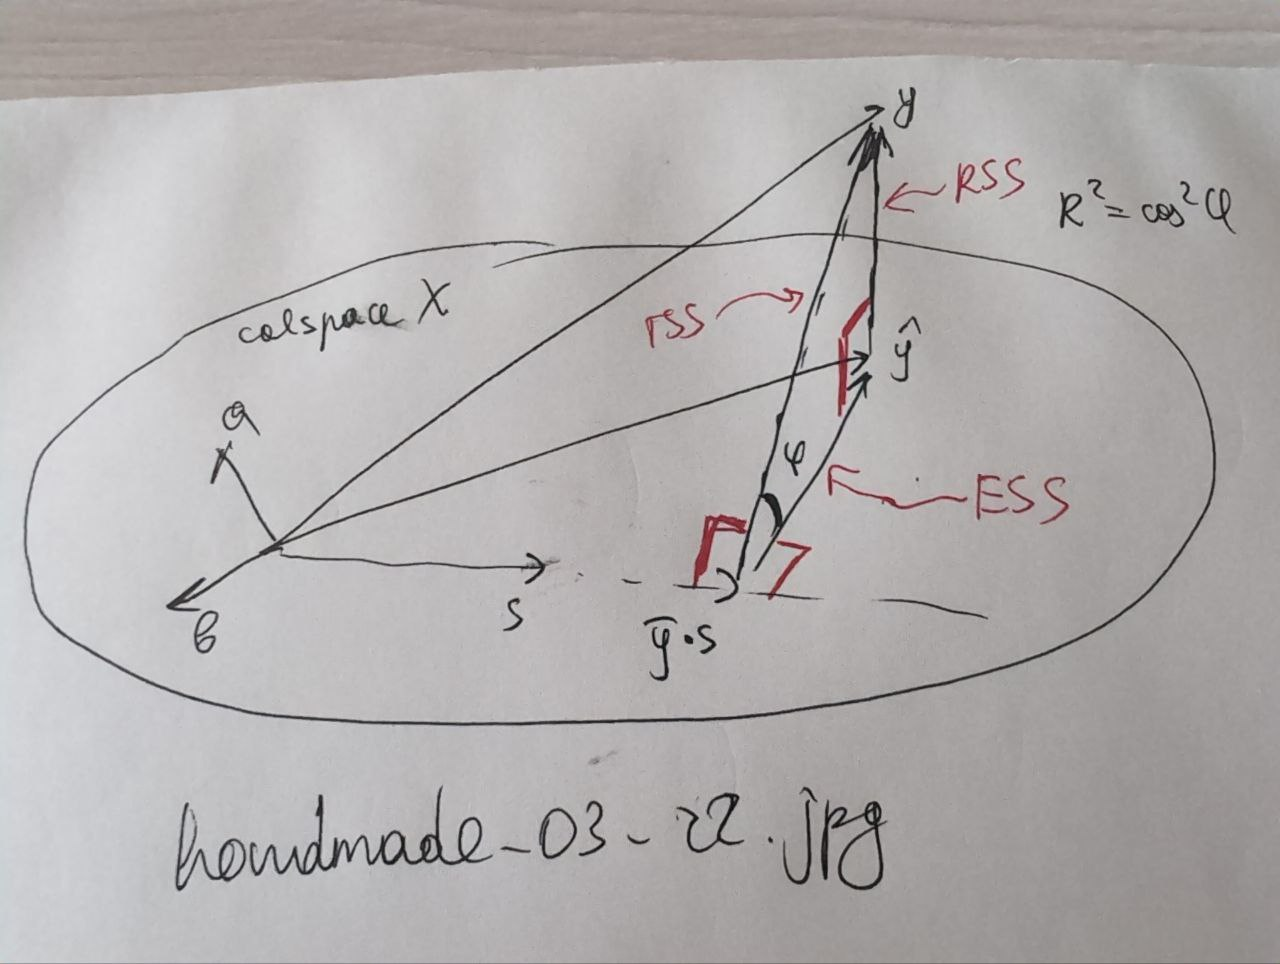
\includegraphics[width=7cm]{handmade/handmade_03_r2.jpg}
\end{minipage}




\subsection{Основные матрицы в линейной регрессии}

Здесь мы приведём основные матрицы, используемые в линейной регрессии и их алгебраические свойства. 

Вспомним определение матрицы-шляпницы:
\begin{definition}[матрица-шляпница]
Матрица $X(X^TX)^{-1} X^T$ часто обозначается буквой $H$ и неформально называется \emph{матрицей-шляпницей} (hat matrix).
Она «надевает» на $y$ шляпку, $Hy = \hat y$.
Формально матрица $H$ также называется матрицей-проектором. 
Она проецирует любой вектор на линейную оболочку всех регрессоров $\Span(\col_1 X, \col_2 X, \dots, \col_k X)$.
\end{definition}

\begin{theorem}
Матрица-проектор $H = X(X^TX)^{-1}X^T$ обладает следующими свойствами:
\begin{enumerate}
    \item $H$ — симметричная, $H^T = H$;
    \item $H$ — идемпотентная, $H^2 = H$;
    \item $\rank H = \trace H = k$, где $k$ — число столбцов матрицы $X$.
\end{enumerate}
\end{theorem}
\begin{proof}

\begin{enumerate}
    \item Симметричность, $H^T = H$:
    \[
    H^T = X(X^{T}X)^{-1}X^{T} = H
    \]
    \item Идемпотентносить, $H^2 = H$:
    \[
    H^2 =  X(X^{T}X)^{-1}(X^{T}X)(X^{T}X)^{-1}X^{T} = X(X^{T}X)^{-1}X^{T} = H
    \]
    \item $\rank H = \trace H = k$:
    \[
    \trace H = \trace (X(X^{T}X)^{-1}X^{T}) = \trace ((X^{T}X)(X^{T}X)^{-1}) = \trace I_k = k.
    \]
    Здесь мы использовали свойство следа $\trace(ABC) = \trace(CAB)$.
    \end{enumerate}
\end{proof}


Определим матрицу $M = I-H$. 
Матрица $M$, как и матрица $H$, является матрицей-проектором. 
Она проецирует любой вектор на ортогональное дополнение к линейной оболочке всех регрессоров $\Span(\col_1 X, \col_2 X, \dots, \col_k X)$. 
Несложно убедиться, что матрица $M$ так же, как и матрица $H$, симметричная и идемпотентная. При этом $\trace M = \trace(I_n - H) = \trace I_n - \trace H = n - k$. 
Проверьте симметричность и идемпотентность матрицы $M$ самостоятельно.


Используя введённые матрицы, выразим вектор остатков в модели $y = X\beta + u$:
\[
\hu = y - \hy = y - Hy = (I - H)y = My = M(X\beta + u) = Mu, 
\]
так как из геометрического смысла матрицы $M$ следует, что $MX = 0$.

Пусть 
$s = 
 \begin{pmatrix}
  1 & 1 & \cdots & 1
 \end{pmatrix}^{T}$  — вектор размерности $[n \times 1]$, состоящий из единиц.
Определим матрицу $\pi = s^{T}(s^{T}s)^{-1}s^{T}$. Матрица $\pi$ — это матрица размерности $[n \times n]$ вида
\[
\pi = \frac{1}{n}
 \begin{pmatrix}
  1 & 1 & \cdots & 1\\
  1 & 1 & \cdots & 1\\
  \cdots & \cdots & \cdots & \cdots \\
  1 & 1 & \cdots & 1
 \end{pmatrix}.
 \]
 
В качестве домашнего упражнения покажите, что для произвольного вектора $c$ размерности $[n \times 1]$ выполнено равенство $\pi \cdot c = \bar c \cdot s$, где $\bar c$ – среднее арифметическое, посчитанное по элементам вектора $c$. 

С помощью новых обозначений $\TSS$, $\ESS$ и $\RSS$ могут быть записаны в матричном виде:

\[
\TSS = (y - \bar{y})^{T}(y - \bar{y}) = (y - \pi y)^{T}(y - \pi y) = ((I - \pi)y)^{T}((I - \pi)y) = y^{T}(I - \pi)^{T}(I-\pi)y = y^{T}(I - \pi)y,
\]
\[
\ESS = (\hat{y} - \bar y)^{T}(\hat{y} - \bar y) = (Hy - \pi y)^{T}(Hy - \pi y) = (y(H - \pi)y)^{T}((H - \pi)y) = y^{T}(H - \pi)^{T}(H - \pi)y = y^{T}(H - \pi)y,
\]
\[
\RSS = (y - \hat{y})^{T}(y - \hat{y}) = (y - H y)^{T}(y - Hy) = ((I - H)y)^{T}(y(I - H)) = y^{T}(I - H)^{T}(I-H)y = y^{T}(I - H)y.
\]

\subsection{Теорема Фриша~—Во!}

% TODO: история про спор с детрендирование и Фриша с Во

Сначала рассмотрим задачу. 
Джеймс Бонд для конспирации строит только регрессии на одну переменную. 
За один раз Джеймс может оценить ровно один коэффициент!
Подобных регрессий он может построить сколь угодно много.
Как может Джеймс Бонд, сохраняя конспирацию, оценить \emph{оба} коэффициента в парной регрессии $\hy_i = \hb_1 + \hb_2 x_i$?

Смотрите! На первом шаге Джеймс Бонд строит регрессию $y$ на константу $s = \begin{pmatrix}
    1 \\
    \vdots \\
    1 
\end{pmatrix}$. 
Он получает прогнозы первого шага $\hy_i = \bar y$.
Остатками первой регрессии являются $y^*_i = y_i - \bar y$.

На втором шаге Джеймс Бонд аналогично строит регрессию $x$ на константу $\one$ и, аналогично, получает остатки $x^*_i = x_i - \bar x$.

И, наконец, на третьем шаге Джеймс строит регрессию полученных остатков $y^*$ на остатки $x^*$,
$\hat y^*_i = \hb x^*_i$.

Оценка коэффициента на третьем шаге равна
\[
\hb = \frac{\sum y_i^* x_i^*}{\sum(x_i^*)^2} = \frac{\sum (y_i - \bar y)(x_i - \bar x)}{\sum (x_i - \bar x)^2}.
\]

Но именно это и есть оценка для $\hb_2$ в парной регрессии $\hy_i = \hb_1 + \hb_2 x_i$!
\[
\hb_2 = \frac{\sum (y_i - \bar y)(x_i - \bar x)}{\sum (x_i - \bar x)^2}.
\]

Это совпадение не случайно! 
Оказывается множественную регрессию с любым количеством регрессоров можно разбить на несколько шагов со вспомогательными регрессиями с меньшим числом регрессоров. 

Вместо непосредственного включения переменной $x$ в качестве регрессора в модель можно сначала «очистить» от переменной $x$ зависимую переменную $y$ и остальные регрессоры,
а затем оценить регрессию для «очищенных» переменных.
Эту идею последовательных регрессий формализует теорема Фриша~— Во~— Ловелла.


\begin{theorem}[Теорема Фриша~— Во~— Ловелла (англ. Frisch–Waugh–Lovell theorem, FWL theorem)]

Рассмотрим два алгоритма. 

Алгоритм $A$: оцениваем регрессию $y$ на полный набор регрессоров $X_1$ и $X_2$ с помощью МНК:
\[
\hy_A = X_1 \hb_1^A  + X_2 \hb_2^A.
\]
Алгоритм $B$: 
\begin{enumerate}
    \item[B1.] Оцениваем регрессию $y$ на часть регрессоров $X_1$ с помощью МНК:
    \[
    \hy_{B} = X_1 \hb_1^{B}.
    \]
    \item[B2.] Оцениваем регрессию каждого столбца из матрицы $X_2$ с помощью МНК:
    \[
    \hat X_2^{B} = X_1 \hb_1^{B}.
    \]
    Уточним, что здесь $\hb_1^B$ — это не вектор, а целая матрица, в которой содержатся оценки регрессии каждого столбца из матрицы $X_2$ на все регрессоры из матрицы $X_1$.
    \item[B3.] Определяем «очищенные» переменные как остатки регрессий первых двух шагов,
    \[
    y^* = y - \hy_B, \quad X_2^* = X_2 - \hat X_2^B.
    \]
    \item[B4.] Оцениваем регрессию для «очищенных переменных»
    \[
    \hy^* = X_2^*\hb_2^B.
    \]
\end{enumerate}

Алгоритмы $A$ и $B$ дают одинаковые оценки коэффициентов $\hb_2^A = \hb_2^B$ и финальные векторы остатков $\hu_A = y - \hy_A = y^* - \hy^* = \hu^*_B$.
\end{theorem}


\begin{proof}
Определим матрицу-шляпницу $H_1$, проецирующую на линейную оболочку столбцов блока $X_1$, и матрицу $M_1 = I - H_1$, проецирующую на ортогональное дополнение к линейной оболочке столбцов $X_1$,
\[
H_1 = X_1(X_1^TX_1)^{-1}X_1^T, \quad M_1 = I - H_1.
\]
По определению, $H_1 X_1 = X_1$ и $M_1 X_1 = 0$.

Возьмём результат выполнения алгоритма $A$
\[
y = X_1 \hb_1^A + X_2 \hb_2^A + \hu_A
\]
и домножим его на матрицу $M_1$:
\[
M_1 y = 0 \cdot \hb_1^A + M_1 X_2 \hb_2^A + M_1 \hu_A
\]

Заметим, что остатки $\hu_A$ алгоритма $A$ ортогональны и регрессорам из блока $X_1$, и регрессорам из блока $X_2$. 
Сначала воспользуемся тем, что остатки $\hu_A$ \emph{уже} лежат в подпространстве, ортогональном регрессорам блока $X_1$. 
Дополнительное проецирование в это подпространство никак их не изменяет, $M_1 \hu_A  = \hu_A$.
Следовательно,
\[
M_1 y  = M_1 X_2 \hb_2^A + \hu_A
\]

Теперь воспользуемся тем, что остатки $\hu_A$ \emph{уже} лежат в подпространстве, ортогональном регрессорам блока $X_2$, поэтому $X_2^T \hu_A = 0$.

Ортогональны ли остатки $\hu_A$ и столбцы матрицы $M_1 X_2$? Проверим!
\[
(M_1 X_2)^T \hu_A = X_2^T M_1^T \hu_A = X_2^T M_1 \hu_A = X_2^T \hu_A = 0.
\]

Остаётся лишь сказать, что умножение на матрицу $M_1$ очищает переменные, $M_1 y = y^*$ и $M_1 X_2 = X_2^*$,
\[
y^* = X_2^* \hb_2^A + \hu_A,
\]
И мы видим идеальное совпадение с разложением алгоритма $B$,
\[
y^* = X_2^* \hb_2^B + \hu^*_B
\]
В силу единственности разложения по ортогональному базису $\hb_2^A = \hb_2^B$ и $\hu_A = \hu^*_B$.
\end{proof}


% TODO: Рассказать, что коэффициенты при стандартизации всех переменных называют частными корреляциями?

% TODO: Чёрный трэк: нелинейный мнк численно?

% TODO Рост R2 c ростом числа регрессоров; рост \RSS с ростом числа наблюдений

\subsection{Кросс-валидация с выкидывание отдельных наблюдений}


\begin{definition}[LOOCV]
Кросс-валидация с поочередным выкидыванием отдельных наблюдений. 
На английском языке она часто сокращается LOOCV (leave one out cross validation).

Рассмотрим модель $y=X\beta + u$. 

Оценим модель без первого наблюдения. Получим МНК-оценки $\hb^{(-1)}$.
С помощью этих оценок спрогнозируем первое наблюдение, получим прогноз $\hat y_1^{CV}$ и ошибку прогноза $\hat u_1^{CV}$.

Вернём первое наблюдение в выборку и удалим второе наблюдение. Получим МНК-оценки $\hb^{(-2)}$.
С помощью этих оценок спрогнозируем второе наблюдение, получим прогноз $\hat y_2^{CV}$ и ошибку прогноза $\hat u_2^{CV}$.

Поступим так с каждым наблюдением. На выходе получим вектор кросс-валидационных прогнозов $\hat y^{CV}$ и вектор кросс-валидационных ошибок прогнозов $\hat u^{CV} = y - \hat y^{CV}$.    
\end{definition}

\begin{theorem}[связь обычных и кросс-валидационных остатков]
Если модель $y=X\beta + u$ оценивается с помощью МНК и проводится кросс-валидации с поочередным выкидыванием отдельных наблюдений, то:
\[
\hat u_i = (1 - H_{ii}) \cdot \hat u_i^{CV},
\]
где $H$ — матрица-шляпница $H = X(X^TX)^{-1}X^T$, $\hat u$ — остатки регрессии, а $\hat u^{CV}$ — кросс-валидационные ошибки прогнозов.
\end{theorem}

Заметим, что сомножитель $(1 - H_{ii}) \in (0;1)$. 
Другими словами, теорема численно формализует интуитивно ожидаемый результат: кросс-валидационные остатки по знаку совпадают с обычными остатками, а по абсолютной величине — больше, так как соответствующее наблюдение не используется при оценивании коэффициента. 

\begin{proof}
Оценим модель без последнего наблюдения, $\hat y^{d} = X^{d} \hb^{d}$. 
Буква $d$ означает не степень, а удаление (deletion) последнего наблюдения,
в частности, вектор $y^d$ содержит $(n-1)$ элемент, а матрица $X^{d}$ имеет размер $[(n-1)\times k]$.

Создадим вектор $y^{*}$, который будет отличаться от $y$ только последним, $n$-м элементом:
вместо настоящего $y_n$ там будет стоять прогноз по модели без последнего наблюдения $\hat y^{d}_n$.

Раз уж мы добавили новую точку лежащую ровно на выборочной регрессии, то при оценки модели
$\hat y^* = X \hat \beta^*$ мы получим в точности старые оценки $\hat \beta^* = \hat \beta^d$. 
Следовательно, и прогнозы эти две модели дают одинаковые, $\hat y_i^* = \hat y_i^d$.

А теперь посмотрим на последний элемент вектора $v = H (y^* - y)$.

С одной стороны, он равен последней строке матрицы $H$ умножить на вектор $(y^* - y)$. 
В векторе $(y^* - y)$ только последний элемент ненулевой, поэтому $v_n = H_{nn} (\hat y^{d}_n - y_n)$.

С другой стороны, мы можем раскрыть скобки, и заметить, что $v = Hy^* - Hy$. 
И окажется, что $v_n = \hat y_n^* - \hat y_n = \hat y_n^d - \hat y_n$.

Отсюда
\[
 \hat y_n^d - \hat y_n = H_{nn} (\hat y_n^d - y_n)
\]

Приводим подобные слагаемые и добавляем слева и справа $y_n$, получаем как раз то, что нужно:
\[
y_n - \hat y_n   = (1 - H_{ii}) (y_n - \hat y_n^d )
\]
\end{proof}


\subsection{Задачи}

% TODO сбросить нумерацию задач 

\begin{problem}
    Оценим  регрессию на константу $y_i = \beta_1 + u_i$ с помощью МНК. 
    Найдите
    \begin{enumerate}
        \item $\hb_1$;
        \item $\hy_i$;
        \item $\ESS$;
        \item $R^2$.
    \end{enumerate}
\end{problem}

\begin{sol}
    
\begin{enumerate}
    \item Задача минимизации для модели регрессии на константу:
    \[
    Q(\hb_1) = \sum_{i=1}^n (y_i - \hb_1) \to \underset{\hb_1}{\min}.
    \]
Условие первого порядка:
\[
\frac{\partial Q}{\partial \hb_1} = -2\sum_{i=1}^n (y_i - \hb_1) = 0.
\]

Решаем уравнение:
\[
\sum_{i=1}^n y_i - n\beta_1 = 0 \implies \hb_1 = \frac{1}{n}\sum_{i=1}^n y_i.
\]


\item Поскольку модель содержит только константу:
\[
\hat{y}_i = \hat{\beta}_1 = \bar{y} \quad \text{для всех } i=1,\dots,n.
\]

\item Вычислим $\ESS$:
\[
\ESS = \sum_{i=1}^n (\hat{y}_i - \bar{y})^2 = \sum_{i=1}^n (\bar{y} - \bar{y})^2 = 0.
\]

\item Вычислим компоненты:
\begin{align*}
TSS &= \sum_{i=1}^n (y_i - \bar{y})^2 \\
ESS &= 0 \\
RSS &= \sum_{i=1}^n (y_i - \hat{y}_i)^2 = TSS \\
\end{align*}

Коэффициент детерминации:
\[
R^2 = \frac{ESS}{TSS} = 0.
\]
\end{enumerate}
\end{sol}

\begin{problem}
Для модели парной линейной регрессии $y_i = \beta_1 + \beta_2 x_i + u_i$ получите оценки коэффициентов $\beta_1$, $\beta_2$ двумя путями:

\begin{enumerate}
    \item используя готовую матричную формулу $\hb = (X^TX)^{-1}X^Ty$;
    \item решая задачу оптимизации методом наименьших квадратов $\sum^n_{i=1} (y_i - \hb_1 - \hb_2 x_i)^2 \to \underset{\hb_1, \hb_2}{\min}.$
\end{enumerate}   
\end{problem}

\begin{sol}
\begin{enumerate}
\item Запишем модель в матричном виде:
\[ y = X\beta + u, \quad
\text{ где }
\quad
X = \begin{pmatrix}
1 & x_1 \\
1 & x_2 \\
\vdots & \vdots \\
1 & x_n
\end{pmatrix}, \quad
y = \begin{pmatrix}
y_1 \\
y_2 \\
\vdots \\
y_n
\end{pmatrix}, \quad
\beta = \begin{pmatrix}
\beta_1 \\
\beta_2
\end{pmatrix}
\]

Вычислим необходимые матрицы:
\[
X^TX = \begin{pmatrix}
n & \sum x_i \\
\sum x_i & \sum x_i^2
\end{pmatrix}, \quad
X^Ty = \begin{pmatrix}
\sum y_i \\
\sum x_i y_i
\end{pmatrix}
\]

Обратная матрица:
\[
(X^TX)^{-1} = \frac{1}{n\sum x_i^2 - (\sum x_i)^2}
\begin{pmatrix}
\sum x_i^2 & -\sum x_i \\
-\sum x_i & n
\end{pmatrix}
\]

МНК-оценка:
\[
\hat{\beta} = (X^TX)^{-1}X^Ty = \frac{1}{n\sum x_i^2 - (\sum x_i)^2}
\begin{pmatrix}
\sum x_i^2 \sum y_i - \sum x_i \sum x_i y_i \\
n \sum x_i y_i - \sum x_i \sum y_i
\end{pmatrix}
\]

Таким образом:
\[
\hat{\beta}_1 = \frac{\sum x_i^2 \sum y_i - \sum x_i \sum x_i y_i}{n\sum x_i^2 - (\sum x_i)^2}
\]
\[
\hat{\beta}_2 = \frac{n \sum x_i y_i - \sum x_i \sum y_i}{n\sum x_i^2 - (\sum x_i)^2}
\]

\item Минимизируем сумму квадратов остатков:
\[
Q(\hat{\beta}_1, \hat{\beta}_2) = \sum_{i=1}^n (y_i - \hat{\beta}_1 - \hat{\beta}_2 x_i)^2 \to \underset{\hb_1, \hb_2}{\min}.
\]

Условия первого порядка:
\[
\frac{\partial Q}{\partial \hat{\beta}_1} = -2\sum (y_i - \hat{\beta}_1 - \hat{\beta}_2 x_i) = 0,
\]
\[
\frac{\partial Q}{\partial \hat{\beta}_2} = -2\sum x_i(y_i - \hat{\beta}_1 - \hat{\beta}_2 x_i) = 0.
\]

Получаем систему нормальных уравнений:
\[
\begin{cases}
n\hat{\beta}_1 + \hat{\beta}_2\sum x_i = \sum y_i, \\
\hat{\beta}_1\sum x_i + \hat{\beta}_2\sum x_i^2 = \sum x_i y_i,
\end{cases}
\]

Решение системы:
\[
\hat{\beta}_2 = \frac{n\sum x_i y_i - \sum x_i \sum y_i}{n\sum x_i^2 - (\sum x_i)^2},
\]
\[
\hat{\beta}_1 = \frac{\sum y_i - \hat{\beta}_2 \sum x_i}{n} = \bar{y} - \hat{\beta}_2 \bar{x}.
\]

Сравним результаты. 
Оба метода дают одинаковые выражения для оценок коэффициентов:
\[
\hat{\beta}_1 = \bar{y} - \hat{\beta}_2 \bar{x}
\]
\[
\hat{\beta}_2 = \frac{\sum (x_i - \bar{x})(y_i - \bar{y})}{\sum (x_i - \bar{x})^2}
\]
\end{enumerate}
\end{sol}

\begin{problem}
    Покажите, что для модели парной линейной регрессии  $y_i = \beta_1 + \beta_2 x_i + u_i$  выполняются следующие свойства:
    \label{task:2lin}
    \begin{enumerate}
        \item $\sum^n_{i=1} \hu_i = 0$;
        \item $\sum^n_{i=1} \hy_i = n \bar{y}$;
        \item $\sum^n_{i=1} \hu_i x_i = 0$;
        \item $\bar{y} = \hb_1 + \hb_2 \bar{x}$
    \end{enumerate}
\end{problem}

\begin{sol}
\begin{enumerate}
    \item Оценки МНК получаются минимизацией суммы квадратов остатков:
\[
Q(\hb_1, \hb_2) = \sum^n_{i=1} (y_i - \hb_1 - \hb_2 x_i)^2.
\]
Условие первого порядка для $\hb_1$:
\[
\frac{\partial Q}{\partial \hb_1} = -2 \sum^n_{i=1} (y_i - \hb_1 - \hb_2 x_i) = 0.
\]
Отсюда:
\[
\sum^n_{i=1} \hu_i = \sum^n_{i=1} (y_i - \hy_i) = 0.
\]

\item Из пункта а):
\[
\sum^n_{i=1} \hu_i = \sum^n_{i=1} (y_i - \hy_i) = 0 \implies \sum^n_{i=1} y_i = \sum^n_{i=1} \hy_i.
\]
Разделив на $n$, получим:
\[
\bar{y} = \frac{1}{n} \sum^n_{i=1} y_i = \frac{1}{n} \sum^n_{i=1} \hy_i = \bar{\hat{y}}.
\]
\item Условие первого порядка для $\hb_2$:
\[
\frac{\partial Q}{\partial \hb_2} = -2 \sum^n_{i=1} (y_i - \hb_1 - \hb_2 x_i) x_i = 0.
\]
Отсюда:
\[
\sum^n_{i=1} \hu_i x_i = \sum^n_{i=1} (y_i - \hy_i) x_i = 0.
\]

\item Из пункта б):
\[
\bar{y} = \frac{1}{n} \sum^n_{i=1} \hy_i = \frac{1}{n} \sum^n_{i=1} (\hb_1 + \hb_2 x_i) = \hb_1 + \hb_2 \bar{x}.
\]
\end{enumerate}
\end{sol}

\begin{problem}
    Для модели парной линейной регрессии  $y_i = \beta_1 + \beta_2 x_i + u_i$

    \begin{enumerate}
        \item в скалярном виде выпишите $\TSS$, $\RSS$, $\ESS$,
        \item покажите, что $\TSS = \RSS + \ESS$.
    \end{enumerate}
\end{problem}

\begin{sol}
\begin{enumerate}
    \item Для модели парной линейной регрессии \( y_i = \beta_1 + \beta_2 x_i + u_i \) найдём все компоненты:

\begin{itemize}
    \item Общая сумма квадратов (Total Sum of Squares, TSS):
    \[
    \TSS = \sum_{i=1}^n (y_i - \bar{y})^2,
    \]
    где \(\bar{y} = \frac{1}{n} \sum_{i=1}^n y_i\) — выборочное среднее зависимой переменной.

    \item Объяснённая сумма квадратов (Explained Sum of Squares, ESS):
    \[
    \text{ESS} = \sum_{i=1}^n (\hat{y}_i - \bar{y})^2,
    \]
    где \(\hat{y}_i = \hat{\beta}_1 + \hat{\beta}_2 x_i\) — предсказанное значение \(y_i\) по оценённой модели.

    \item Остаточная сумма квадратов (Residual Sum of Squares, RSS):
    \[
    \text{RSS} = \sum_{i=1}^n (y_i - \hat{y}_i)^2,
    \]
    где \(y_i - \hat{y}_i = \hat{u}_i\) — остаток модели.
\end{itemize}

\item Докажем равенство $\TSS = \ESS + \RSS$.

Начнём с определения $\TSS$ и разложим отклонение $y_i - \bar{y}$ на две составляющие:

\[
y_i - \bar{y} = (y_i - \hat{y}_i) + (\hat{y}_i - \bar{y}).
\]

Возведём обе части в квадрат и просуммируем по всем наблюдениям:

\[
\sum_{i=1}^n (y_i - \bar{y})^2 = \sum_{i=1}^n \left[ (y_i - \hat{y}_i) + (\hat{y}_i - \bar{y}) \right]^2.
\]

Раскроем квадрат в правой части:

\[
\sum_{i=1}^n (y_i - \bar{y})^2 = \sum_{i=1}^n (y_i - \hat{y}_i)^2 + \sum_{i=1}^n (\hat{y}_i - \bar{y})^2 + 2 \sum_{i=1}^n (y_i - \hat{y}_i)(\hat{y}_i - \bar{y}).
\]

Заметим, что:
\begin{itemize}
    \item \(\sum_{i=1}^n (y_i - \hat{y}_i)^2 = \RSS\),
    \item \(\sum_{i=1}^n (\hat{y}_i - \bar{y})^2 = \ESS\),
    \item перекрёстное произведение \(\sum_{i=1}^n (y_i - \hat{y}_i)(\hat{y}_i - \bar{y}) = 0\) (доказательство ниже).
\end{itemize}

Докажем, что $\sum_{i=1}^n (y_i - \hat{y}_i)(\hat{y}_i - \bar{y}) = 0$.
Заметим, что:
\begin{itemize}
    \item \(\hat{y}_i = \hat{\beta}_1 + \hat{\beta}_2 x_i\), где \(\hat{\beta}_1 = \bar{y} - \hat{\beta}_2 \bar{x}\) (из условий первого порядка МНК).
    \item \(\sum_{i=1}^n \hat{u}_i = \sum_{i=1}^n (y_i - \hat{y}_i) = 0\) (свойство остатков МНК).
    \item \(\sum_{i=1}^n \hat{u}_i x_i = 0\) (условие ортогональности в МНК).
\end{itemize}

Теперь раскроем перекрёстное произведение:

\[
\sum_{i=1}^n (y_i - \hat{y}_i)(\hat{y}_i - \bar{y}) = \sum_{i=1}^n \hat{u}_i (\hat{\beta}_1 + \hat{\beta}_2 x_i - \bar{y}) =
\]

(подставим $\hat{\beta}_1 = \bar{y} - \hat{\beta}_2 \bar{x}$):

\[
= \sum_{i=1}^n \hat{u}_i (\bar{y} - \hat{\beta}_2 \bar{x} + \hat{\beta}_2 x_i - \bar{y}) = \sum_{i=1}^n \hat{u}_i \hat{\beta}_2 (x_i - \bar{x}) = \hat{\beta}_2 \sum_{i=1}^n \hat{u}_i (x_i - \bar{x}) =
\]
\[
= \hat{\beta}_2 \left( \sum_{i=1}^n \hat{u}_i x_i - \bar{x} \sum_{i=1}^n \hat{u}_i \right) = \hat{\beta}_2 (0 - \bar{x} \cdot 0) = 0.
\]

Таким образом, перекрёстное произведение равно нулю, и равенство $\TSS = \ESS + \RSS$ доказано.
\end{enumerate}
\end{sol}

\begin{problem}
    Для модели парной линейной регрессии без константы $y_i = \beta_1 x_i + u_i$ покажите, что в общем случае

    \begin{enumerate}
        \item $\sum^n_{i=1} \hu_i \neq 0$
        \item $\bar{y} \neq \hb_1 \bar{x}$
        \item $\TSS \neq \RSS + \ESS$
        \item $R^2 = 1 - \frac{RSS}{TSS} \notin [0, 1]$
    \end{enumerate}
\end{problem}

\begin{sol}
\begin{enumerate}
    \item В модели с константой выполняется $\sum \hat{u}_i = 0$, но в модели \textbf{без константы}:
    \[ \sum_{i=1}^n \hat{u}_i = \sum_{i=1}^n y_i - \hat{\beta_1} \sum_{i=1}^n x_i. \]
    Эта разность равна нулю только если $\sum y_i = \hat{\beta} \sum x_i$, что выполняется не всегда.

    \textbf{Контрпример:}
    Пусть $x = (1, 2)^T$, $y = (3, 5)^T$. Тогда:
    \[ \hat{\beta_1} = \frac{1 \cdot 3 + 2 \cdot 5}{1^2 + 2^2} = \frac{13}{5} = 2.6 \]
    Остатки:
    \[ \hat{u}_1 = 3 - 2.6 \cdot 1 = 0.4 \]
    \[ \hat{u}_2 = 5 - 2.6 \cdot 2 = -0.2 \]
    Сумма остатков: $0.4 - 0.2 = 0.2 \neq 0$.

    \item В модели \textbf{без константы}:
    \[ \bar{y} = \frac{1}{n} \sum_{i=1}^n y_i, \]
    \[ \hat{\beta_1} \bar{x} = \hat{\beta_1} \cdot \frac{1}{n} \sum_{i=1}^n x_i. \]
    Из пункта «а» следует, что в общем случае $\sum y_i \neq \hat{\beta_1} \sum x_i$, значит:
    \[ \bar{y} \neq \hat{\beta_1} \bar{x}. \]

    \item В модели \textbf{с константой} выполняется разложение:
    \[ \text{TSS} = \text{ESS} + \text{RSS}, \]
    где:
    \begin{itemize}
        \item $\text{TSS} = \sum (y_i - \bar{y})^2$ (общая сумма квадратов),
        \item $\text{ESS} = \sum (\hat{y}_i - \bar{y})^2$ (объясненная сумма квадратов),
        \item $\text{RSS} = \sum \hat{u}_i^2$ (остаточная сумма квадратов).
    \end{itemize}

    В модели \textbf{без константы} это разложение \textbf{не выполняется}, так как:
    \[ \sum \hat{u}_i \neq 0 \implies \text{выборочная ковариация между } \hat{y}_i \text{ и } \hat{u}_i \text{ не равна нулю}. \]
    Следовательно:
    \[ \text{TSS} \neq \text{ESS} + \text{RSS}. \]

    \item Коэффициент детерминации $R^2$ вычисляется по формуле:
    \[
    R^2 = 1 - \frac{\text{RSS}}{\text{TSS}}.
    \]
    Поскольку для модели без константы $\text{TSS} \neq \text{ESS} + \text{RSS}$, то $R^2$ может выходить за пределы $[0, 1]$ если $\text{RSS} > \text{TSS}$, то $R^2 < 0$.
\end{enumerate}
\end{sol}


\begin{problem}
    Покажите, что для регрессии вида $y_i = \beta_1 + \beta_2 x_i + u_i$ $R^2$ обладает следующими свойствами:

    \begin{enumerate}
    \item $R^2 = \sCorr^2(y, x), $ где $\sCorr^2(y, x)$ -- выборочный коэффициент корреляции.

    \item $R^2$ для заданной регрессии и $R^2$ для регрессии $x_i = \alpha_1 + \alpha_2 y_i + v_i$ равны.

    \item Если $\hb_1 = 0,$ то $R^2 = 0.$    
    \end{enumerate}
    
\end{problem}

\begin{problem}
    Пусть мы оценили модель $y_i = \beta_1 + \beta_2 x_i + u_i$ с помощью МНК.

    \begin{enumerate}
    \item Если данные оказались центрированными, что вы можете сказать о $\hb_1$?
    \item Ко всем наблюдениям $x_i$ прибавили 15. Как изменятся $\hb_1, \hb_2$?
    \item Все наблюдения $x_i$ увеличили в 5 раз, что произойдёт с $\hb_1, \hb_2$ и $\hy_i$?
    \end{enumerate}
\end{problem}


\begin{sol}
\begin{enumerate}
    \item Если данные центрированы ($\bar{x} = 0$, $\bar{y} = 0$), то:
    \[
    \hat{\beta}_1 = \bar{y} - \hat{\beta}_2 \bar{x} = 0 - \hat{\beta}_2 \cdot 0 = 0
    \]

    \item Ко всем $x_i$ прибавили 15. Обозначим новый регрессор как $x_i' = x_i + 15$. Тогда новое среднее равно $\bar{x}' = \bar{x} + 15$.
    \begin{itemize}
        \item Оценка наклона не изменится:
        \[
        \hat{\beta}_2' = \frac{\sum (x_i' - \bar{x}')(y_i - \bar{y})}{\sum (x_i' - \bar{x}')^2} = \frac{\sum (x_i - \bar{x})(y_i - \bar{y})}{\sum (x_i - \bar{x})^2} = \hat{\beta}_2.
        \]
        \item Оценка константы изменится:
        \[
        \hat{\beta}_1' = \bar{y} - \hat{\beta}_2' \bar{x}' = \bar{y} - \hat{\beta}_2 (\bar{x} + 15) = \hat{\beta}_1 - 15 \hat{\beta}_2.
        \]
    \end{itemize}

    \item Все $x_i$ увеличили в 5 раз. Обозначим новый регрессор как $x_i'' = 5x_i$. Тогда новое среднее равно $\bar{x}'' = 5\bar{x}$.
    \begin{itemize}
        \item Оценка наклона изменится:
        \[
        \hat{\beta}_2'' = \frac{\sum (x_i'' - \bar{x}'')(y_i - \bar{y})}{\sum (x_i'' - \bar{x}'')^2} = \frac{5 \sum (x_i - \bar{x})(y_i - \bar{y})}{25 \sum (x_i - \bar{x})^2} = \frac{\hat{\beta}_2}{5}.
        \]
        \item Оценка константы не изменится:
        \[
        \hat{\beta}_1'' = \bar{y} - \hat{\beta}_2'' \bar{x}'' = \bar{y} - \frac{\hat{\beta}_2}{5} \cdot 5\bar{x} = \bar{y} - \hat{\beta}_2 \bar{x} = \hat{\beta}_1.
        \]
        \item Прогнозные значения:
        \[
        \hat{y}_i'' = \hat{\beta}_1'' + \hat{\beta}_2'' x_i'' = \hat{\beta}_1 + \frac{\hat{\beta}_2}{5} \cdot 5x_i = \hat{\beta}_1 + \hat{\beta}_2 x_i = \hat{y}_i.
        \]
    \end{itemize}
\end{enumerate}

\end{sol}


\begin{problem}
    
    Рассмотрим регрессию $\hy_i = \hb_1 z_i + \hb_2 x_i$.
    Все исходные данные поместим в матрицу $X$ и вектор $y$:
    \[
    X = \begin{pmatrix}
    z_1 & x_1 \\
    \vdots & \vdots \\
    z_n & x_n \\
    \end{pmatrix} \;
    y = \begin{pmatrix}
    y_1 \\
    \vdots \\
    y_n \\
    \end{pmatrix}
    \]
    \begin{enumerate}
      \item Выпишите явно матрицы $X^T$, $X^T y$, $X^T X$, $y^T X$, $y^T z$ и укажите их размер.
      \item Выпишите условия первого порядка для оценок $\hb_1$ и $\hb_2$ по методу наименьших квадратов.
      \item Запишите эти же условия в виде линейной системы
      \[
    \begin{cases}
    \hb_1 \cdot \ldots + \hb_2 \cdot \ldots = \ldots \\
    \hb_1 \cdot \ldots + \hb_2 \cdot \ldots = \ldots \\
    \end{cases}
      \]
      \item Как упростится данная система для регрессии $\hy_i = \hb_1 + \hb_2 x_i$?
      \item Запишите систему условий первого порядка с помощью матрицы $X$ и вектора $y$;
    \end{enumerate}    
\end{problem}

\begin{problem}
    Рассмотрим модель $y_i = \beta_1 + \beta_2 x_{i} + u_i$, 
    где
    \[
    x = \begin{pmatrix} 
      1 \\ 
      2 \\ 
      3 \\ 
    \end{pmatrix}, \quad
    y = \begin{pmatrix} 1 \\ 1 \\ 4 \end{pmatrix}, \quad
    \beta = \begin{pmatrix} \beta_1 \\ \beta_2 \end{pmatrix}, \quad
    u = \begin{pmatrix} u_1 \\ u_2 \\ u_3 \end{pmatrix}
    \]   
    
    \begin{enumerate}
    \item Укажите число наблюдений
    \item Найдите $\TSS = \sum_{i=1}^n (y_i - \bar y)^2$.
    \item С помощью МНК найдите оценку для вектора неизвестных коэффициентов без использования матриц.
    \item Перепишите модель в матричном виде и получите оценку коэффициентов через матричные формулы для МНК (убедитесь, что оценки совпали :)).
    \item Найдите $\RSS = \sum_{i=1}^n (y_i - \hy_i)^2$.
    \item Чему равен $R^2$ в модели? Прокомментируйте полученное значение с точки зрения качества оценённого уравнения регрессии.
    \end{enumerate}
\end{problem}

\begin{sol}
\begin{enumerate}
    \item Количество строк в векторе $y$ равно 3. Следовательно, $n=3$.
    
    \item Вычислим среднее значение $\bar{y}$:
    \[
    \bar{y} = \frac{1 + 1 + 4}{3} = 2.
    \]
    
    Тогда общая сумма квадратов:
    \[
    \text{TSS} = (1-2)^2 + (1-2)^2 + (4-2)^2 = 1 + 1 + 4 = 6.
    \]
    
    \item Формулы для МНК-оценок:
    \[
    \hat{\beta}_2 = \frac{\sum (x_i - \bar{x})(y_i - \bar{y})}{\sum (x_i - \bar{x})^2},
    \]
    \[
    \hat{\beta}_1 = \bar{y} - \hat{\beta}_2 \bar{x}.
    \]
    
    Вычислим необходимые величины:
    \[
    \bar{x} = \frac{1 + 2 + 3}{3} = 2,
    \]
    \[
    \sum (x_i - \bar{x})(y_i - \bar{y}) = (1-2)(1-2) + (2-2)(1-2) + (3-2)(4-2) = 1 + 0 + 2 = 3,
    \]
    \[
    \sum (x_i - \bar{x})^2 = (1-2)^2 + (2-2)^2 + (3-2)^2 = 1 + 0 + 1 = 2.
    \]
    
    Тогда оценки:
    \[
    \hat{\beta}_2 = \frac{3}{2} = 1.5,
    \]
    \[
    \hat{\beta}_1 = 2 - 1.5 \times 2 = -1.
    \]
    
    \item Матрица регрессоров и вектор зависимой переменной:
    \[
    X = \begin{pmatrix}
    1 & 1 \\
    1 & 2 \\
    1 & 3 \\
    \end{pmatrix}, \quad
    Y = \begin{pmatrix} 1 \\ 1 \\ 4 \end{pmatrix}.
    \]
    
    МНК-оценка коэффициентов:
    \[
    \hat{\beta} = (X^T X)^{-1} X^T Y.
    \]
    
    Вычислим:
    \[
    X^T X = \begin{pmatrix}
    3 & 6 \\
    6 & 14 \\
    \end{pmatrix}, \quad
    X^T Y = \begin{pmatrix} 6 \\ 15 \end{pmatrix},
    \]
    \[
    (X^T X)^{-1} = \frac{1}{6} \begin{pmatrix}
    14 & -6 \\
    -6 & 3 \\
    \end{pmatrix},
    \]
    \[
    \hat{\beta} = \frac{1}{6} \begin{pmatrix}
    14 \times 6 - 6 \times 15 \\
    -6 \times 6 + 3 \times 15 \\
    \end{pmatrix} = \begin{pmatrix} -1 \\ 1.5 \end{pmatrix}.
    \]
    
    Результаты совпали с предыдущим пунктом.
    
    \item Прогнозные значения:
    \[
    \hat{y}_1 = -1 + 1.5 \times 1 = 0.5,
    \]
    \[
    \hat{y}_2 = -1 + 1.5 \times 2 = 2,
    \]
    \[
    \hat{y}_3 = -1 + 1.5 \times 3 = 3.5.
    \]
    
    Остаточная сумма квадратов:
    \[
    \text{RSS} = (1-0.5)^2 + (1-2)^2 + (4-3.5)^2 = 0.25 + 1 + 0.25 = 1.5.
    \]
    
    \item Формула для $R^2$:
    \[
    R^2 = 1 - \frac{\text{RSS}}{\text{TSS}} = 1 - \frac{1.5}{6} = 0.75.
    \]
    
    Интерпретация: модель объясняет 75\% вариации зависимой переменной, что говорит о хорошем качестве подгонки модели.
\end{enumerate}
\end{sol}

\begin{problem}
    Рассмотрим модель $y_i = \beta_1 + \beta_2 x_{i} + \beta_3 z_i + u_i$, 
    где
    \[
    X = \begin{pmatrix} 
      1 & 0 & 0 \\ 
      1 & 0 & 0 \\ 
      1 & 0 & 0 \\ 
      1 & 1 & 0 \\ 
      1 & 1 & 1 
    \end{pmatrix}, \quad
    y = \begin{pmatrix} 1 \\ 2 \\ 3 \\ 4 \\ 5 \end{pmatrix}, \quad
    \beta = \begin{pmatrix} \beta_1 \\ \beta_2 \\ \beta_3 \end{pmatrix}, \quad
    u = \begin{pmatrix} u_1 \\ u_2 \\ u_3 \\ u_4 \\ u_5  \end{pmatrix}
    \]
       
    Для удобства расчётов даны матрицы:
    \[
    X^TX = \begin{pmatrix} 
      5 & 2 & 1 \\ 
      2 & 2 & 1\\ 
      1 & 1 & 1 
    \end{pmatrix},
    (X^TX)^{-1}= \begin{pmatrix} 
      1/3 & -1/3 & 0 \\ 
      -1/3 & 4/3 & -1 \\ 
      0 & -1 & 2 \end{pmatrix}.
    \]   
    
    \begin{enumerate}
    \item Укажите число наблюдений
    \item Укажите число регрессоров в модели, учитывая свободный член.
    \item Найдите $\TSS = \sum_{i=1}^n (y_i - \bar y)^2$.
    \item С помощью МНК найдите оценку для вектора неизвестных коэффициентов.
    \item Найдите вектор прогнозов $\hy$.
    \item Найдите $\RSS = \sum_{i=1}^n (y_i - \hy_i)^2$.
    \item Чему равен $R^2$ в модели? Прокомментируйте полученное значение с точки зрения качества оценённого уравнения регрессии.
    \end{enumerate}
\end{problem}

\begin{sol}
\begin{enumerate}
    \item Количество строк в матрице $X$ равно 5, следовательно, $n = 5$.
    
    \item В модель включена  свободный член и две объясняющие переменные ($x$ и $z$), то есть $k = 3$.
    
    \item Вычислим среднее значение $\bar{y}$:
    \[
    \bar{y} = \frac{1 + 2 + 3 + 4 + 5}{5} = 3.
    \]
    
    Тогда общая сумма квадратов:
    \[
    \text{TSS} = (1-3)^2 + (2-3)^2 + (3-3)^2 + (4-3)^2 + (5-3)^2 = 4 + 1 + 0 + 1 + 4 = 10.
    \]
    
    \item Используем матричную формулу МНК:
    \[
    \hat{\beta} = (X^T X)^{-1} X^T y.
    \]
    
    Умножим обратную матрицу на $X^T y$:
    \[
    X^T y = \begin{pmatrix} 1+2+3+4+5 \\ 0+0+0+4+5 \\ 0+0+0+0+5 \end{pmatrix} = \begin{pmatrix} 15 \\ 9 \\ 5 \end{pmatrix},
    \]
    \[
    (X^T X)^{-1} X^T y = \begin{pmatrix} 
      1/3 & -1/3 & 0 \\ 
      -1/3 & 4/3 & -1 \\ 
      0 & -1 & 2 \end{pmatrix} 
      \begin{pmatrix} 15 \\ 9 \\ 5 \end{pmatrix} = 
      \begin{pmatrix} 
      5 - 3 + 0 \\ 
      -5 + 12 - 5 \\ 
      0 - 9 + 10 \end{pmatrix} = 
      \begin{pmatrix} 2 \\ 2 \\ 1 \end{pmatrix}.
    \]
    
    \item Вычислим вектор прогнозов $\hat{y} = X \hat{\beta}$:
    \[
    \hat{y} = \begin{pmatrix} 
      1 & 0 & 0 \\ 
      1 & 0 & 0 \\ 
      1 & 0 & 0 \\ 
      1 & 1 & 0 \\ 
      1 & 1 & 1 
    \end{pmatrix}
    \begin{pmatrix} 2 \\ 2 \\ 1 \end{pmatrix} = 
    \begin{pmatrix} 2 \\ 2 \\ 2 \\ 4 \\ 5 \end{pmatrix}.
    \]
    
    \item Остаточная сумма квадратов:
    \[
    \text{RSS} = (1-2)^2 + (2-2)^2 + (3-2)^2 + (4-4)^2 + (5-5)^2 = 1 + 0 + 1 + 0 + 0 = 2.
    \]
    
    \item Формула для $R^2$:
    \[
    R^2 = 1 - \frac{\text{RSS}}{\text{TSS}} = 1 - \frac{2}{10} = 0.8.
    \]
\end{enumerate}
\end{sol}

\begin{problem}

    Константин оценивает влияние продаж на заработную плату менеджера: $salary_i = \beta_1 + \beta_2 sales_i + u_i.$ Он оценил коэффициенты с помощью МНК, нашёл $R^2_1$ и ему не понравился результат. 

    \begin{enumerate}
        \item Тогда Константин выкинул одно из наблюдений, переоценил модель и получил $R^2_2$. Может ли он сравнить модели по $R^2$ и выбрать наилучшую?
        \item Константин добавил в модель регрессор числа созвонов с начальством $sinks_i$. Покажите, что $R^2$ у данной регрессии вырастет в любом случае.
        \item  Константин слышал, что некоторые исследователи логарифмируют зарплаты перед включением в модель. Объясните, можно ли сравнивать по $R^2$ регрессии $salary_i$ и $log(salary_i)$ на один и тот же набор регрессоров?
    \end{enumerate}
\end{problem}

\begin{problem}
    Я очень хочу тут реальный датасет с точными датами рождения людей :)
\end{problem}

\begin{problem}
    Рассмотрим модель множественной регрессии
    \[
    y = X\beta + u,
    \]
    где $X$ — матрица признаков размерности $[n \times k]$.
    Определим матрицу $M = I - X(X^TX)^{-1}X^T$. Покажите, что
    \begin{enumerate}
    \item матрица $M$ симметричная;
    \item матрица $M$ идемпотентная;
    \item $\trace M = n - k$.
    \end{enumerate}
\end{problem}

\begin{sol}
   \begin{enumerate}
\item Вычислим транспонированную матрицу $M$:
\[
M^T = \left(I_n - X(X^T X)^{-1}X^T\right)^T = I_n^T - \left(X(X^T X)^{-1}X^T\right)^T = I_n - X\left((X^T X)^{-1}\right)^T X^T.
\]
Поскольку \( X^T X \) симметрична, то \( (X^T X)^{-1} \) также симметрична:
\[
\left((X^T X)^{-1}\right)^T = (X^T X)^{-1}.
\]
Следовательно,
\[
M^T = I_n - X(X^T X)^{-1}X^T = M.
\]
Таким образом, \( M \) симметрична.

\item Матрица $M$ называется идемпотентной, если $M^2 = M$.

Вычислим $M^2$:

\begin{align}
M^2 &= \left(I_n - X(X^T X)^{-1}X^T\right)\left(I_n - X(X^T X)^{-1}X^T\right) \\
&= I_n - 2X(X^T X)^{-1}X^T + X(X^T X)^{-1}X^T X(X^T X)^{-1}X^T.
\end{align}

Упростим последнее слагаемое:
\[
X(X^T X)^{-1}X^T X(X^T X)^{-1}X^T = X(X^T X)^{-1}(X^T X)(X^T X)^{-1}X^T = X(X^T X)^{-1}X^T.
\]
Подставим обратно:
\[
M^2 = I_n - 2X(X^T X)^{-1}X^T + X(X^T X)^{-1}X^T = I_n - X(X^T X)^{-1}X^T = M.
\]
Таким образом, $M$ идемпотентна.

\item Используем свойства следа матрицы:

\begin{align}
    \trace(M) &= \trace\left(I_n - X(X^T X)^{-1}X^T\right) \\
&= \trace(I_n) - \trace\left(X(X^T X)^{-1}X^T\right).
\end{align}


След единичной матрицы равен её размеру, $\trace(I_n) = n$. 
Для второго слагаемого воспользуемся свойством следа \( \trace(AB) = \trace(BA) \):
\[
\trace\left(X(X^T X)^{-1}X^T\right) = \trace\left((X^T X)^{-1}X^T X\right) = \trace(I_k) = k.
\]
Таким образом,
\[
\trace (M) = n - k.
\]
   \end{enumerate}
\end{sol}

\begin{problem}
Пусть 
$s = 
 \begin{pmatrix}
  1 & 1 & \cdots & 1
 \end{pmatrix}^{T}$ — вектор размерности $[n \times 1]$, состоящий из единиц.
Определим матрицу $\pi = s^{T}(s^{T}s)^{-1}s^{T}$. Матрица $\pi$ — это матрица размерности $[n \times n]$ вида
\[
\pi = \frac{1}{n}
 \begin{pmatrix}
  1 & 1 & \cdots & 1\\
  1 & 1 & \cdots & 1\\
  \cdots & \cdots & \cdots & \cdots \\
  1 & 1 & \cdots & 1
 \end{pmatrix}.
 \]
 
Покажите, что $\pi \cdot c = \bar c \cdot s$, где $c$ — произвольный вектор размерности $[n \times 1]$; $\bar c$ – среднее арифметическое, посчитанное по элементам вектора $c$.
\end{problem}

\begin{sol}

Вычислим произведение $\pi \cdot c$:
\[
\pi \cdot c = \frac{1}{n} 
\begin{pmatrix} 
1 & 1 & \cdots & 1 \\
1 & 1 & \cdots & 1 \\
\vdots & \vdots & \ddots & \vdots \\
1 & 1 & \cdots & 1 
\end{pmatrix}
\begin{pmatrix} c_1 \\ c_2 \\ \vdots \\ c_n \end{pmatrix}
\]
Умножение матрицы на вектор дает:
\[
\pi \cdot c = \frac{1}{n} 
\begin{pmatrix} 
\sum_{i=1}^n c_i \\
\sum_{i=1}^n c_i \\
\vdots \\
\sum_{i=1}^n c_i 
\end{pmatrix}
= \frac{1}{n} \sum_{i=1}^n c_i \cdot 
\begin{pmatrix} 1 \\ 1 \\ \vdots \\ 1 \end{pmatrix} = 
\begin{pmatrix} \bar{c} \\ \bar{c} \\ \vdots \\ \bar{c} \end{pmatrix}.
\]
По определению среднего значения:
\[
\pi \cdot c = \bar{c} \cdot \one,
\]
где $\one = (1, 1, \dots, 1)^T$.

Таким образом, мы показали, что умножение матрицы $\pi$ на произвольный вектор $c$ дает вектор, все элементы которого равны среднему значению элементов вектора $c$.
\end{sol}

\section{Предпосылки о математическом ожидании и дисперсии}
В этой главе мы познакомимся с понятиями независимости и линейной независимости, расчётом математических ожиданий, ковариаций и дисперсий в матричном виде.

Добавим в метод наименьших квадратов ряд статистических предпосылок на ожидание и дисперсию.

Сформулируем и докажем теорему Гаусса~- Маркова (которая пообещает, что МНК-оценки будут обладать свойствами несмещённости и эффективности).

\subsection{Иерархия зависимостей случайных величин}


Напомним определение наилучшей линейной аппроксимации.
\begin{definition}[наилучшая линейная аппроксимация]
Наилучшее линейное приближение величины $r$ с помощью величины $s$ — это линейная функция от $s$,
\[
\BestLin(r \mid s) = \beta_1 + \beta_2 s,
\]
где константы $\beta_1$ и $\beta_2$ находятся из решения задачи оптимизации
$\E((r - \BestLin(r, s)^2) \to \min_{\beta_1, \beta_2}$.
При решении задачи оказывается, что
\[
\beta_1 = \E(r) - \frac{\Cov(r, s)}{\Var(s)} \E(s), \quad \beta_2 = \frac{\Cov(r, s)}{\Var(s)}.
\]
\end{definition}

\begin{definition}[линейная независимость]
Величины $r$ и $s$ называются линейно-независимыми, если $\BestLin(r \mid s) = \E(r)$.
\end{definition}
Некоторые авторы считают условие $\Cov(r, s) = 0$ определением линейной независимости.

Можно выделить три степени независимости случайных величин. 
Рассмотрим их на примере пары произвольных величин $r$ и $s$.

\begin{tikzpicture}[node distance=2cm] % Set node distance
    % Define nodes
    \node[rectangle, draw=orange, line width=1.5pt] (indep) {$r$ и $s$ независимы}; 
    \node[rectangle, draw=orange, line width=1.5pt, right=2cm of indep] (indep2) {$\Cov(h_1(r), h_2(s)) = 0$ для любых функций $h_1$ и $h_2$}; 

    \node[rectangle, draw=orange, line width=1.5pt, below of=indep] (noreg) {$\E(r \mid s) = \E(r)$}; 
    \node[rectangle, draw=orange, line width=1.5pt, right=3cm of noreg] (noreg2) {$\Cov(r, h(s)) = 0$ для любой функции $h$}; 

    \node[rectangle, draw=orange, line width=1.5pt, align=center, below of=noreg] (nocov) {$r$ и $s$ линейно-независимы, \\
    $\BestLin(r \mid s) = \E(r)$}; 
    \node[rectangle, draw=orange, line width=1.5pt, right=3cm of nocov] (nocov2) {$\Cov(r, s) = 0$}; 

    % Connect nodes with arrows
    \draw[{Latex[length=5mm, width=4mm]}-{Latex[length=5mm, width=4mm]}, line width=1pt, double distance=3pt] (indep) -- (indep2);
    \draw[{Latex[length=5mm, width=4mm]}-{Latex[length=5mm, width=4mm]}, line width=1pt, double distance=3pt] (noreg) -- (noreg2);
    \draw[{Latex[length=5mm, width=4mm]}-{Latex[length=5mm, width=4mm]}, line width=1pt, double distance=3pt] (nocov) -- (nocov2);

    \draw[-{Latex[length=5mm, width=4mm]}, line width=1pt, double distance=3pt] (indep) -- (noreg);
    \draw[-{Latex[length=5mm, width=4mm]}, line width=1pt, double distance=3pt] (noreg) -- (nocov);
\end{tikzpicture}

Далее напомним определение независимых случайных величин.
\begin{definition}[независимость случайных величин]
Cлучайные величины $r$ и $s$ называются \emph{независимыми}, если 
для любых\footnote{Не совсем любых, требуется измеримость множеств. 
В рамках нашего курса мы не будем обращать внимания на данный нюанс.} числовых множеств $A$ и $B$ независимы события $\{r \in A\}$ и $\{s \in B\}$:
\[
\P(r \in A, s \in B) = \P(r \in A) \cdot \P(s \in B)
\]
\end{definition}

Из независимости величин $r$ и $s$ следует, что информация, известная об $s$, никак не помогает угадывать значение $r$. Поэтому условное математическое ожидание для $r$ равно безусловному. Точно также из независимости $r$ и $s$ следует $\E(s \mid r) = \E(s)$. Обратное утверждение неверно, что показывает контрпример ниже.

\begin{problem}
    Покажем, что из равенства условного и безусловного математических ожиданий не следует независимость случайных величин. Пусть дискретные случайные величины $r$ характеризуют погоду (-1 снег, 1 солнце, 0 дождь), $s$ — наличие зонта (0 нет или 1 есть) и ниже приведена таблица их совместного распределения.
    
    \begin{tabular}{|l|l|l|l|}
    \hline
      & 1/3 & 1/3 & 1/3 \\ \hline
    r & -1  & 1   & 0   \\ \hline
    s & 0   & 0   & 1   \\ \hline
    \end{tabular}  

    
    
    \begin{sol}
    Уже по формулировке подозреваем, что величины зависимые :).

    Найдём условное ожидание зонта при условии, что мы видим погоду на улице: \( \E(s \mid r) = \begin{cases} 0 \text{ если } r\in \{-1,  1\}, \\
    1, \text{ если } r = 0. \end{cases}\) Получается, что информация о погоде помогает предсказать наличие зонтика, события не являются независимыми.

    Найдём ожидания о погоде за окном, если вы можете наблюдать наличие или отсутствие зонта у человека:  \( \E(r \mid s) = \begin{cases} (-1) \times 1/6 + 1 \times 1/6 = 0, \text{ если } s = 0, \\
    0, \text{ если } s = 1. \end{cases}\).

    Обычное безусловное ожидание погоды на улице: \( \E(r) = (-1) \times 1/3 + 1 \times 1/3 + 0 \times 1/3 = 0\) 

    Получается, что \( \E(r \mid s) = \E(r) = 0, \) но события зависимы.
    \end{sol}
\end{problem}

Вернемся к тому факту, что из равенства условного и безусловного математических ожиданий следует нулевая ковариация. Используя закон повторных математических ожиданий  \( \Cov(r, s) = \E(rs) - \E(r)\E(s) = \E(\E(rs \mid s)) - \E(r)\E(s) = \E(s\E(r \mid s)) - \E(r)\E(s) = \E(r)\E(s) - \E(r)\E(s) = 0.\)


\begin{problem}
    Из нулевой ковариации не следует равенство условного и безусловного математических ожиданий (и тем более не следует независимость). Пусть случайная величина $s$ имеет равномерное распределение на отрезке $[-1; 1]$, а $r = s^2$.

    \begin{sol}

    Напоминаем, что для равномерно распределённой случайной величины \(\E(s) = \frac{-1+1}{2} = 0, pdf(s) = \frac{1}{1 - (-1)} = \frac{1}{2}.\)
    
    \(\E(r \mid s) = \E(s^2 \mid s) = s^2 \neq 0\) в общем случае.

    При этом \(\Cov(r, s) = \E(rs) - \E(r)\E(s) = \E(s^3) - \E(s^2) \times 0 = \E(s^3).\)

    Математическое ожидание сложной функции \( \E(g(x)) = \int^r_b g(x) pdf(x) dx, \text{если } x \in [a, b].\)
    
    Найдём \(\E(s^3) = \int^{1}_{-1} s^3 pdf(s) ds = \int^{1}_{-1} s^3 \frac{1}{2} ds = \frac{1}{8} s^4 | ^1_{-1} = 0.\) Значит, мы получили нулевую ковариацию у зависимых случайных величин.    
    \end{sol}
\end{problem}

\subsubsection*{Вывод}
Существуют независимые случайные величины, но на ???

\subsection{Ожидание и ковариационная матрица }

Любопытный читатель снова может заглянуть в  «Поваренную книга любителя матриц» Петерсона и Педерсона. \cite{petersen2012matrix}.

Пусть $r$ — случайный вектор размерности $[n \times 1]$, $s$ — случайный вектор размерности $[k \times 1]$, $A$ и $b$ — неслучайные матрица и вектор соответственно, имеющие подходящие размерности.

Математическим ожиданием случайного вектора $r$ называется вектор
\[
\E(r) = \begin{pmatrix}
	\E(r_1)  \\
	\E(r_2)  \\
        \dots \\
        \E(r_n)
      \end{pmatrix}.
\]

Ковариационная матрица вектора $r$ определяется следующим образом:
\[
\Var(r) = \begin{pmatrix}
	\Cov(r_1,r_1) & \Cov(r_1,r_2) & \dots & \Cov(r_1,r_n) \\
	\Cov(r_2,r_1) & \Cov(r_2,r_2) & \dots & \Cov(r_2,r_n) \\
        \dots & & \dots & \dots\\
        \Cov(r_n,r_1) & \Cov(r_n,r_2) & \dots & \Cov(r_n,r_n) \\
      \end{pmatrix}.
\]

Ковариационная матрица векторов $r$ и $s$ определяется следующим образом:
\[
\Cov(r,s) = \begin{pmatrix}
	\Cov(r_1,s_1) & \Cov(r_1,s_2) & \dots & \Cov(r_1,s_k) \\
	\Cov(r_2,s_1) & \Cov(r_2,s_2) & \dots & \Cov(r_2,s_k) \\
        \dots & \dots & \dots & \dots\\
        \Cov(r_n,s_1) & \Cov(r_n,s_2) & \dots & \Cov(r_n,s_k) \\
      \end{pmatrix}.
\]

Свойства вектора математических ожиданий и ковариационной матрицы:
\begin{enumerate}
    \item $\E(Ar+b) = A\E(r)+b$
    \item $\Cov(r,s) = \E(rs^T)-\E(r)\E(s^T)$
    \item $\Cov(Ar+b,s) = A\Cov(r,s)$
    \item $\Cov(r,As+b) = \Cov(r,s)A^T$
    \item $\Var(r)=\Cov(r,r) = \E(rr^T)-\E(r)\E(r^T)$
    \item $\Var(Ar+b) = A\Var(r)A^T$
    \item $\E(r^T Ar) = \trace(A\Var(r))+\E(r^T) A\E(r)$  
    \item Если вектора $r$ и $s$ имеют одинаковый размер, то
    $\Var(r + s) = \Var(r) + \Var(s) + \Cov(r, s) + \Cov(s, r)$
\end{enumerate}

Условные ожидание и дисперсия определяются аналогично и обладают аналогичными свойствами.
Главное — не забывать ставить вертикальную палочку!

Например, 
\todo[inline]{написать пример}

\subsection{Теорема Гаусса~— Маркова для парной линейной регрессии}

Вернёмся к модели парной линейной регрессии, для которой мы научились получать оценки $\hb_1, \hb_2$ методом наименьших квадратов:
\[ y_i = \beta_1 + \beta_2 x_i + u_i. \]

Мы убедились, что практически для любых данных в $y$ и $x$ оценки технически могут быть получены (кроме случая, когда все $x_i$ являются одинаковыми и в знаменателе для $\hb_1 = \frac{\sum (x_i - \bar{x})(y_i - \bar{y)}}{\sum(x_i - \bar{x})^2}$ произойдёт деление на ноль). 

При этом мы ничего не говорили о качестве полученных оценок, а оказывается, что МНК-оценки далеко не всегда будут "хорошими" с точки зрения несмещённости, состоятельности и эффективности.

Сформулируем теорему, которая будет отвечать на вопрос, в каких случаях можно доверять оценкам, полученным методом наименьших квадратов.

\begin{theorem}[Гаусс~— Марков для парной линейной регрессии]
Если 

\begin{enumerate}[label=\arabic*.]
    \item Линейность: модель линейна по параметрам: $y_i = \beta_1 + \beta_2 x_i + u_i$;
    \item Экзогенность: условное ожидание случайных ошибок равно нулю: \( \E(u_i \mid x_1, x_2, \dots, x_n) = 0\);
    \item Гомоскедастичность: условная дисперсия случайных ошибок постоянна: \( \Var(u_i \mid x_1, \dots, x_n) = \sigma_u^2, \quad 0 < \sigma_u^2 < \infty \);
    \item Линейная независимость: $\E(u_i u_j \mid x_1, x_2, \dots, x_n) = 0$;
    \item Оценки $\hb_1, \hb_2$ получены методом наименьших квадратов;
\end{enumerate}

то
\begin{enumerate}[label=(\alph*)]
    \item Оценки $\hb_1, \hb_2$ являются линейными по $y$;
    \item Оценки $\hb_1, \hb_2$ является условно несмещёнными, $\E(\hb_i \mid x_1, \ldots x_n) = \beta_i$ и несмещёнными, $\E(\hb_i) = \beta_i$;
    \item Оценка любого коэффициента $\hb_i$ является наиболее эффективной в классе линейных несмещённых оценок.
\end{enumerate}
\end{theorem}

\todo[inline]{куда-то присобачить состоятельность, тогда появятся конечные четвёртые моменты? $E[X^4] < \infty, \quad E[Y^4] < \infty$}

Перед тем, как перейти к доказательству, обсудим, что означает каждая предпосылка и какие ограничения она накладывает.

\subsubsection*{Линейность модели}

В данном случае подразумевается, что модель является линейной по параметрам $\beta_1, \beta_2$. Это является достаточно сильным упрощением реальности. Мы не можем быть уверенными, что например, зарплата $y$ линейно возрастает по опыту $x$. 

Если на самом деле окажется, что мы пытаемся оценить нелинейные эффекты с помощью линейной модели, то качество оценок будет печальным и никакая теорема Гаусса-Маркова уже не поможет. Мы в дальнейшем ещё будем рассуждать о том, как заподозрить нелинейность в ваших данных.

В качестве утешения уже сейчас можно строить нелинейные по $x$ модели: например \( y_i = \beta_1 + \beta_2 x_i^2 + u_i \) удовлетворяет условию теоремы Гаусса~- Маркова. Модель \( y_i = \beta_1 + e^{\beta_2 x_i} + u_i \) не удовлетворяет условию, так как нелинейна по $\beta_2$. 

\subsubsection*{Экзогенность}
Нулевое условное математическое ожидание (или экзогенность) выписывается в форме \[ E(u_i \mid x_1, x_2, \dots, x_n) = 0. \]

\todo[inline]{связка с другим разделом}

Мы предполагаем, что в имеющихся данных по $x_i$ не осталось никакой информации, которая помогла бы выдать полезный, отличный от нуля прогноз для $u_i$. По предыдущим разделам мы можем выписать более слабую версию этой предпосылки: \( E[u_i \mid x_i] = 0 \) и даже ещё более слабые $\E(u_i) = 0$ и $\Cov(x, u) = 0.$ В такой форме чуть легче понять, что в реальной жизни можно считать нарушением предпосылки об экзогенности. 

Так как \( E(u_i \mid x_i)] = 0 \Rightarrow \Cov{(x, u)} = 0,  \) значит по правилам построения отрицаний \(\Cov(x, u) \neq 0  \Rightarrow E(u_i \mid x_i) \neq 0.\) Если получится придумать, по какой причине $u$ в вашей модели коррелирует с $x$, вы точно нарушаете предпосылку. Например, вы всё ещё оцениваете влияние опыта работы $x$ на зарплату $y$. Все факторы, влияющие на заработную плату, которые не были учтены в модели, автоматически перемещаются в ошибки (возраст, пол, интеллект, стрессоустойчивость, коммуникабельность и т.д.). Тот же возраст часто коррелирует с опытом работы $x$, поэтому в такой парной линейной регрессии нарушается предпосылка об экзогенности (или, иными словами, присутствует эндогенность).

Нарушение предпосылки об экзогенности одно из самых распространённых. Всегда можно придумать регрессоры, которые забыли или не смогли включить в модель, а они коррелируют с уже имеющимися регрессорами. Мы отдельно вернёмся к этой теме в следующих разделах.

\subsubsection*{Гомоскедастичность}

Условная дисперсия случайной ошибки постоянна (гомоскедастичность):

\[ \Var(u_i \mid x_1, \dots, x_n) = \sigma_u^2, \quad 0 < \sigma_u^2 < \infty \]

На рисунке \ref{fig:homohet} приведены примеры для иллюстрации гомоскедастичности и гетероскедастичности. В случае гетероскедастичности разброс $y$ выше при больших $x$, что намекает о зависимости дисперсии ошибок от регрессора. В гомоскедастичность иногда непросто поверить: для той же регрессии зарплаты на опыт работы наверняка можно предположить, что при отсутствии опыта сотрудники будут получать похожие офферы. По мере получения опыта одинаково долго проработавшие в компании сотрудники могут уже получать существенно разные зарплаты из-за иных, неучтённых пока в модели факторов. Это приводит к тому, что некоторые исследователи заранее не верят в гомоскедастичность и предпринимают меры по коррекции результатов оценивания.

\begin{figure}[h]
    \centering
    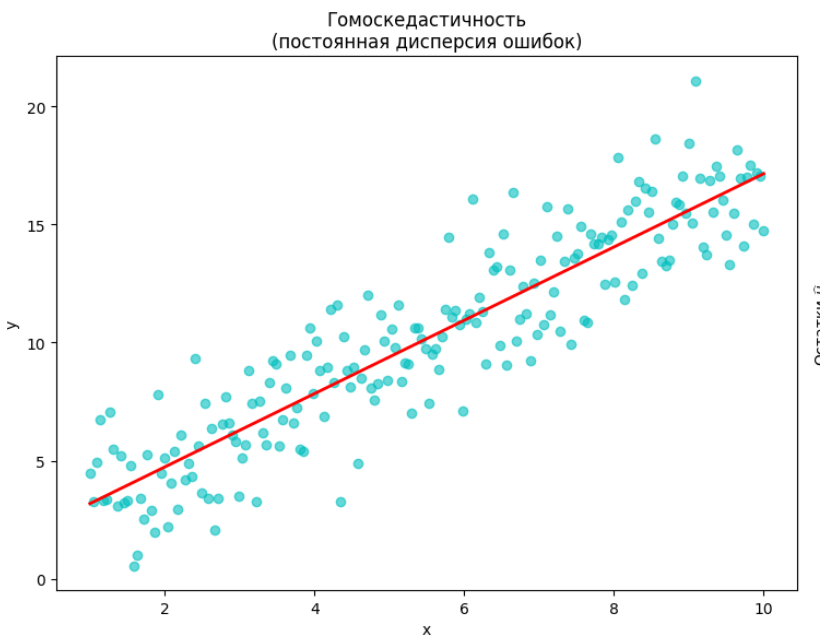
\includegraphics[width=0.4\linewidth]{figures/homosq.png}
    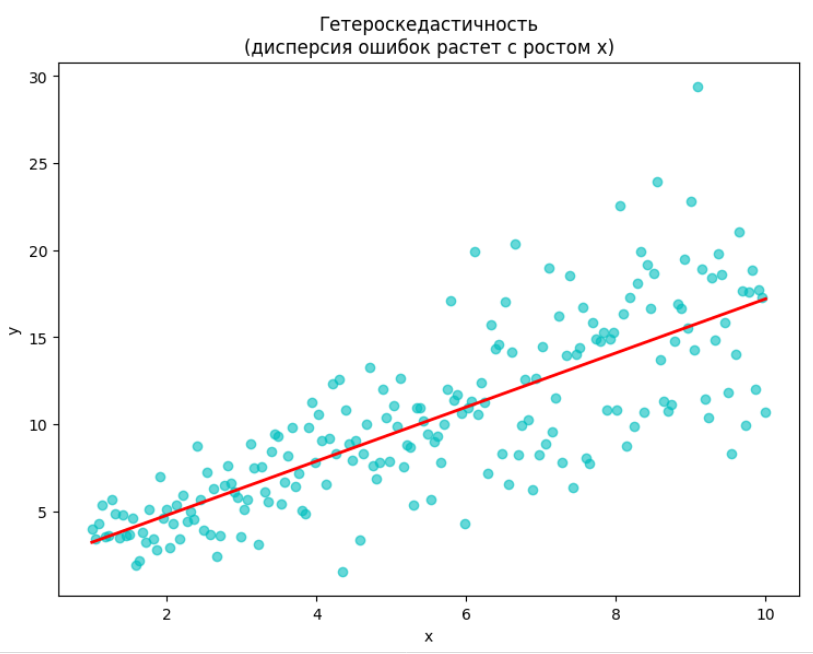
\includegraphics[width=0.4\linewidth]{figures/heterosq.png}
    %\caption{Caption}
    \label{fig:homohet}
\end{figure}

% Текст на странице 2 отсутствует или не распознан.
Во-первых, где в нашем МНК-оценивании используется гомоскедастичность в парной линейной регрессии \( y_i = \beta_1 + \beta_2 x_i + u_i \)? 

\begin{proof}
Мы уже знаем оценку углового коэффициента \[\hat{\beta}_1 = \frac{\sum (x_i - \bar{x})(y_i - \bar{y})}{\sum (x_i - \bar{x})^2} = \frac{\sum y_i (x_i - \bar{x})}{\sum (x_i - \bar{x})^2} = \frac{\sum (\beta_0 + \beta_1 x_i + u_i)(x_i - \bar{x})}{\sum (x_i - \bar{x})^2} = \]

\[= \frac{\beta_0 \sum (x_i - \bar{x}) + \beta_1 \sum x_i (x_i - \bar{x}) + \sum u_i (x_i - \bar{x})}{\sum (x_i - \bar{x})^2}
    = \beta_1 + \frac{\sum u_i (x_i - \bar{x})}{\sum (x_i - \bar{x})^2}\]

Дисперсия оценки \( \hat{\beta}_1: \)
        \[ \Var(\hat{\beta}_1 \mid x_1, x_2, \ldots x_n) = \Var\left( \frac{\sum (x_i - \bar{x}) u_i}{\sum (x_i - \bar{x})^2} \;\middle|\;  x_1, x_2, \ldots x_n \right) = \frac{1}{\left( \sum (x_i - \bar{x})^2 \right)^2} \Var\left( \sum (x_i - \bar{x}) u_i \;\middle|\; x_1, x_2, \ldots x_n \right)\]
Так как наблюдения независимы и случайные ошибки независимы, дисперсия суммы равна сумме дисперсий:
        \[ \Var(\hat{\beta}_1 \mid x_1, x_2, \ldots x_n) = \frac{\sum (x_i - \bar{x})^2 \Var(u_i \mid x_1, x_2, \ldots x_n)}{\left( \sum (x_i - \bar{x})^2 \right)^2} = \frac{\sigma_u^2}{\sum (x_i - \bar{x})^2}. \]
\end{proof}
Такую красивую короткую формулу для теоретической дисперсии оценки углового коэффициента мы получаем только в предпосылке о постоянстве дисперсии случайной ошибки. Без неё пришлось бы делать предположение о том, как ведёт себя ошибка для каждого значений регрессора (чем мы тоже будем заниматься далее).

Что будет, если предположить гомоскедастичность там, где её нет? Показано, что расчёты \textbf{в условиях гомоскедастичности обычно недооценивают} дисперсию оценок коэффициентов. Это приводит к завышенным стандартным ошибкам и проблемам в тестировании гипотез:

\todo[inline]{надо ссылку пруф}

Например, для тестирования \( H_0: \beta_1 = 0 \) против \( H_1: \beta_1 \neq 0 \) с использованием t-статистики мы получим \[ t_{\text{stat}} = \frac{\hb_1 - 0}{s.e.(\hb_1)} \]

Заниженная стандартная ошибка \( s.e.(\hb_1) \) приведёт к слишком большому значению статистики и, значит, к большей вероятности отвергнуть гипотезу о незначимости коэффициента. Получается, что расчёты при гомоскедастичности могут ошибочно говорить о значимости регрессора. В разделе о гетероскедастичности мы будем говорить о том, как можно исправить ситуацию и проводить более пессимистичное тестирование гипотез.

\subsubsection*{Линейная независимость}

Под линейной независимостью подразумевается, что

\[ \E(u_i u_j \mid x_1, x_2, \dots, x_n) = 0\]

В более слабой форме в предыдущем разделе это можно записать как $\Cov(u_i, u_j \mid x_1, x_2, \dots, x_n) = 0$  $\forall i \neq j.$ Это свойство можно считать автоматически выполненным, если перед нами независимая выборка наблюдений. Тогда все неучтённые факторы, влияющие на зарплату человека $i$, не связаны с неучтёнными факторами человека $j$. 

Когда эта предпосылка не выполняется: например, выборка состоит из сотрудников одной компании, в которой опытные сотрудники сговорились и забирают себе все премии, а неопытные ничего не получают. Получается, что в необъяснённых факторах для зарплаты будет корреляция определённого знака в зависимости от опыта работы.

\todo[inline]{ну не самый удачный пример?}

Теперь, когда мы поняли, какой смысл кроется за предпосылками об экзогенности, гомоскедастичности и линейной независимости наблюдений, перейдем к следствиям теоремы. Оценки должны получаться несмещённые и наиболее эффективные в классе линейных.


В иностранной литературе для простоты запоминания используется аббревиатура BLUE, best linear unbiased estimator. Хорошие оценки подобны хорошему подвенечному платью,
\begin{quotation}
Something Olde, Something New, Something Borrowed, Something Blue, A Sixpence in your Shoe.    
\end{quotation}

\subsubsection*{Несмещённость}

Если предпосылка об экзогенности $\E(u_i \mid x_1, x_2, \ldots x_n) = 0$ выполняется, то оценка получается \textbf{несмещённая}. Можно надеяться на то, что она попала недалеко от истинного значения параметра и поэтому имеет какой-то физический смысл (а значит, её можно \textbf{интерпретировать}):

\begin{proof}
В парной линейной регрессии \( y_i = \beta_1 + \beta_2 x_i + u_i \) мы уже знаем оценку углового коэффициента \[\hat{\beta}_1 = \beta_1 + \frac{\sum u_i (x_i - \bar{x})}{\sum (x_i - \bar{x})^2}\]

Вспомним определение несмещённости:
\[ \E(\hat{\beta}_1 \mid x_1, x_2, \ldots x_n) = \E\left( \beta_1 + \frac{\sum u_i (x_i - \bar{x})}{\sum (x_i - \bar{x})^2} \;\middle|\; x_1, x_2, \ldots x_n \right) = \beta_1 + \frac{\sum (x_i - \bar{x}) \E(u_i \mid x_1, x_2, \ldots x_n)}{\sum (x_i - \bar{x})^2} \]

При условии \( \E(u_i \mid x_1, x_2, \ldots x_n) = 0 \), получаем:
\( \E[\hat{\beta}_1 \mid x_1, x_2, \ldots x_n] = \beta_1 \).

По закону повторного математического ожидания \( \E(\E[\hat{\beta}_1 \mid x_1, x_2, \ldots x_n))= \E(\hb_1) =  \beta_1 \)
\end{proof}

\subsubsection*{Линейность}

Оценку \( \hb_1 \) можно представить как линейную комбинацию \( y_i \):
\[\hb_1 = \frac{\sum (x_i - \bar{x}) y_i}{\sum (x_i - \bar{x})^2} = \sum a_i y_i, \text{ где } a_i = \frac{x_i - \bar{x}}{\sum (x_i - \bar{x})^2}. \]

Таким образом, \( \hb_1 \) -- линейная по $y$ оценка.

\subsubsection*{Эффективность}
Под эффективностью мы подразумеваем, что для любой несмещённой и линейной по $y$ оценки $\hb^{alt}$ выполняется $\Var(\hb^{alt}_1) \ge \Var(\hb_1)$

\begin{proof}
    Пусть \[ \hb_1 = \sum a_i y_i = \sum a_i (\beta_0 + \beta_1 x_i + u_i) 
    = \beta_0 \sum a_i + \beta_1 \sum a_i x_i + \sum a_i u_i.\]
    $a_i$ -- это какие-то комбинации из $x_1, x_2, \ldots x_n$, поэтому      
    \[\E(\hb_1 \mid x_1, x_2, \ldots x_n) = \beta_0 \sum a_i + \beta_1 \sum a_i x_i + \sum a_i E(u_i \mid x_1, x_2, \ldots x_n] = \beta_0 \sum a_i + \beta_1 \sum a_i x_i \]

    Для несмещённости \( \E(\hb_1 \mid x_1, x_2, \ldots x_n) = \beta_1, \) значит 
    \[
    \begin{cases}
        \sum a_i = 0, \\
        \sum a_i x_i = 1.
    \end{cases}
    \]

    Альтернативная оценка $\hb_1^{alt} = \sum a_i^{alt} y_i$ тоже несмещённая, значит
    \[
    \begin{cases}
        \sum a_i^{alt} = 0, \sum (a_i - a_i^{alt}) = 0\\
        \sum a_i^{alt} x_i = 1, \sum (a_i - a_i^{alt}) x_i = 0.
    \end{cases}
    \]

    Дисперсия МНК-оценки в условиях гомоскедастичности:
    \[\Var(\hb_1 \mid x_1, x_2, \ldots x_n) = \Var\left( \sum a_i u_i \mid x_1, x_2, \ldots x_n \right) = \sum a_i^2 \Var(u_i \mid x_1, x_2, \ldots x_n)) = \sigma_u^2 \sum a_i^2
    \]

    Аналогично \(\Var( \hb_1^{alt} \mid x_1, x_2, \ldots x_n) = \sigma_u^2 \sum (a_i^{alt})^2.\)

    Осталось понять, можем ли мы утвержать, что \( \sum (a_i^{alt})^2 \ge \sum a_i^2\)?

    \tdplotsetmaincoords{40}{120}
    \begin{tikzpicture}[tdplot_main_coords]
    
    \coordinate (O) at (0,0,0);
    \coordinate (haty) at (-0.9,3);
    \coordinate (1) at (-1.3,1.2);
    \coordinate (a) at (1,-1.5);
    \coordinate (x) at (1, 1.4);
    
    \tdplotsetcoord{S}{10}{35}{0}  % икс
    \tdplotsetcoord{P}{7}{30}{90} % игрек
    \tdplotsetcoord{aalt}{7}{-25}{60} % игрек
    
    \draw[->] (O) -- (P) node[anchor=north west]{$y$};
    \draw (0,0.5) ellipse (4.5cm and 1cm);    
    \draw[->] (O) -- (haty) node[anchor=north east]{\small $\hat y$};
    \draw[->] (O) -- (a) node[anchor=north east]{\small $a$};
    \draw[->] (O) -- (x) node[anchor=south west]{\small $x$};
    \draw[->] (O) -- (1) node[anchor=north west]{\small $1$};
    \draw[->] (O) -- (aalt) node[anchor=north west]{\small $a^{alt}$};
    \draw[dashed, <-] (P) -- (haty) node[above=1.5cm, xshift=0.3cm]{\small $\hat u = y - \hat{y}$};
    \draw[dashed, <-] (a) -- (aalt) node[above=-3cm, xshift=-1cm]{\small $a-a^{alt}$};
    
    \tkzMarkRightAngle[size=0.15](P,haty,O);
    \tkzMarkRightAngle[size=0.15](O,a,aalt);
    
    \end{tikzpicture}

    Оказывается, можем. Вектор $a$ является суммой вектора $x$ и вектора констант (который прячется в $\bar{x}$). Поэтому $a$ лежит в плоскости регрессоров модели. Судя по $\sum (a_i - a_i^{alt}) = 0, \sum (a_i - a_i^{alt})x_i = 0$, вектор $a - a^{alt}$ ортогонален вектору констант и вектору $x$, значит, ортогонален плоскости. Тогда вектор $a^{alt}$ -- соединяющая концы двух векторов гипотенуза, длина которой не меньше катетов, значит \( \sum (a_i^{alt})^2 \ge \sum a_i^2.\)
    
    Если не очень нравится стереометрия, можно воспользоваться раскрытием скобок:

    Пусть \( \hb_1^{alt} = \sum (a_i + d_i) y_i \). Её дисперсия:
    \[ \Var(\hb^{alt}_1 \mid x_1, x_2, \ldots x_n) = \sigma_u^2 \sum (a_i + d_i)^2 \]
    
    \[ \sum (a_i + d_i)^2 = \sum a_i^2 + \sum d_i^2 + 2 \sum a_i d_i = \sum a_i^2 + \sum d_i^2 \geq \sum a_i^2 \quad (\text{т.к. } \sum a_i d_i = 0)  \]
    \[\sum a_i d_i = \sum \frac{(x_i - \bar{x})}{\sum (x_i - \bar{x})^2} d_i = \frac{\sum x_i d_i - \bar{x} \sum d_i}{\sum (x_i - \bar{x})^2} = 0\] 
    \[ \text{ т. к. } \sum d_i = \sum (a_i - a_i^{alt})  = 0 и \sum x_i d_i = \sum (a_i - a_i^{alt}) x_i = 0 \]
\end{proof}
    
\subsubsection*{Состоятельность}

    Состоятельность оценки: при увеличении объёма выборки оценка сходится по вероятности к истинному значению параметра:
    \[ \hat{\beta}_n \xrightarrow{P} \beta \quad \text{или} \quad \plim_{n \to \infty} \hat{\beta}_n = \beta \]
    Это означает, что для любого \( \varepsilon > 0 \):
    \[ \lim_{n \to \infty} P(|\hat{\beta}_n - \beta| > \varepsilon) = 0 \]

    \begin{proof} В нашем случае:
    \[ \hat{\beta}_1 = \frac{\sum (x_i - \bar{x})(y_i - \bar{y})}{\sum (x_i - \bar{x})^2} \]


% Текст на странице 9 отсутствует или не распознан.

    \[\plim \hb_1 = \frac{\Cov(X, Y)}{\Var(X)} = \frac{\Cov(X, \beta_0 + \beta_1 X + u)}{\Var(X)} \\
    = \frac{\Cov(X, \beta_1 X) + Cov(X, u)}{\Var(X)} = \beta_1 + \frac{\Cov(X, u)}{\Var(X)}\]
    
    При выполнении условия экзогенности \( \Cov(X, u) = 0 \), получаем:
\[ \plim \hb_1 = \beta_1 \]
    \end{proof}
\subsection{Теорема Гаусса~— Маркова в общем виде}

Модель множественной регрессии в матричном виде выглядит следующим образом:
\[y = X\beta + u.\]

Чтобы исследовать свойства полученной точечной оценки $\hb$ нам потребуются предпосылки о математическом ожидании и ковариационной матрице вектора $u$.

Мы предположим, что случайные ошибки в среднем равны нулю, а именно,
\[
\E(u \mid X) = 0.
\]

Предпосылку о математическом ожидании можно записать и в скалярном виде,
\[
\E(u_i \mid X) = 0, \quad \text{ при } \forall i \in \{1, \dots, n\}.
\]

Важно пояснить смысл введённой предпосылки. При оценивании связи между регрессорами $X$ и переменной $y$ мы не предполагаем, что величины $u$ и $X$ независимы. В ошибки модели попадают все те факторы, которые мы забыли включить в регрессию. Эти факторы могут быть взаимосвязаны с тем, что в регрессию всё же попало. Мы делаем более слабое предположение лишь о бесполезности всей собранной в $X$ информации для угадывания $u$ (и следующей из неё линейной независимости между ошибками и регрессорами, в том числе о нулевой ковариации).

\begin{theorem}[Гаусс~— Марков]
Если 
\gaussmarkov
то
\begin{enumerate}[label=(\alph*)]
    \item Оценка $\hb$ является линейной по $y$;
    \item Оценка $\hb$ является условно несмещённой, $\E(\hb \mid X) = \beta$ и несмещённой, $\E(\hb) = \beta$;
    \item Оценка любого коэффициента $\hb_j$ является наиболее эффективной в классе линейных несмещённых оценок. 
\end{enumerate}
\end{theorem}

Что означает «эффективная в классе линейных несмещённых оценок»?
Это означает, что у любой другой линейной по $y$ несмещённой оценки $\hb^{\alt}_j$ дисперсия не меньше, чем у МНК-оценки.
\[
\Var(\hb_j \mid X) \leq \Var(\hb^{\alt}_j \mid X).
\]

Вывод теоремы можно усилить: для любой линейной комбинации коэффициентов $w^T \beta$ МНК-оценка $w^T \hb$ эффективнее альтернативной оценки $w^T \hb^{\alt}$, то есть
\[
\Var(w^T\hb_j \mid X) \leq \Var(w^T \hb^{\alt}_j \mid X).
\]

\begin{proof}
Линейность оценки по $y$ видна прямо из её формулы, $\hb = (X^TX)^{-1}X^Ty$.

Проверим условную несмещённость, 
\[
\E(\hb \mid X) = \E((X^TX)^{-1}X^Ty \mid X) = (X^TX)^{-1}X^T\E(y \mid X).
\]
Для удобства посчитаем $\E(y \mid X)$ отдельно,
\[
\E(y \mid X) = \E(X\beta + u \mid X) = X\beta + \E(u \mid X) = X\beta.
\]
И теперь завершаем вычисление $\E(\hb \mid X)$:
\[
\E(\hb \mid X) = (X^TX)^{-1}X^T\E(y \mid X) = (X^TX)^{-1}X^TX\beta = \beta.
\]
Мы доказали условную несмещённость оценки, $\E(\hb \mid X) = \beta$.
Безусловная несмещённость следует из свойства условного ожидания,
\[
\E(\hb) = \E(\E(\hb \mid X)) = \E(\hb) = \beta.
\]

Эффективность МНК-оценок — это реинкарнация теоремы Пифагора. 
Мы увидим, что дисперсия МНК-оценки — это квадрат длины катета, 
дисперсия альтернативной несмещённой оценки — квадрат длины гипотенузы.

Для примера рассмотрим оценку первого коэффициента бета, $\hb_1$.
Доказательство не меняется ни капли, если рассмотреть оценку другого коэффициента, скажем, $\hb_7$ или даже оценку произвольной линейной комбинацию коэффициентов бета, например, $\hb_1 + \hb_2 + \hb_3$.

Итак, у нас есть две оценки, $\hb_1$ и $\hb_1^{\alt}$. 
Обе они линейны по $y$, следовательно, $\hb_1 = a^T y$ и $\hb_1^{\alt} = a^T_{\alt} y$.


Замечаем, что $\Var(\hb_1 \mid X) = \sigma^2 a^Ta$, и $\Var(\hb_1^{\alt}) = \sigma^2 a_{\alt}^Ta_{\alt}$. 
То есть дисперсии пропорциональны квадратам длин векторов $a$ и $a_{\alt}$. 
Осталось доказать, что вектор $a$ не длиннее вектора $a_{\alt}$ :)

Для этого мы докажем, что вектор $a_{\alt}$ — это гипотенуза, а вектор $a$ — катет. 
Нам нужно доказать, что вектор $a - a_{\alt}$ перпендикулярен вектору $a$.

Разобъём доказательство перпендикулярности $a$ и $a-a_{\alt}$ на два шага:

Шаг 1. Вектор $a - a_{\alt}$ перпендикулярен любому столбцу матрицы $X$.

Шаг 2. Вектор $a$ является линейной комбинацией столбцов матрицы $X$.


\todo[inline]{здесь простая картинка с теоремой Пифагора!}




Приступаем к шагу 1. Обе оценки несмещённые, поэтому для любых $\beta$ должно выполняться:

\[
\E(\hb_1 \mid X) = \E(\hb_1^{\alt} \mid X)
\]

Переносим всё в левую сторону:

\[
\E((a^T - a^T_{\alt})(X\beta + u) \mid X) = 0
\]

Получаем, что для любых $\beta$ должно быть выполнено условие:

\[
(a - a_{\alt})^T X\beta = 0
\]

Это возможно только, если вектор $(a - a_{\alt})^T X$ равен нулю. 
Следовательно, вектор $(a - a_{\alt})$ перпендикулярен любому столбцу $X$.


Приступаем к шагу 2.

Вспоминаем, что $\hat \beta = (X^T X)^{-1}X^T y = Ay$. Следовательно, нужная строка весов $a^T$ — 
это первая строка в матрице $(X^TX)^{-1}X^T$. 
Замечаем, что выражение имеет вид $A \cdot X^T$. 

Вспоминаем из линейной алгебры, что при умножении матриц $AB$ получается матрица $C$, 
на которую можно взглянуть несколькими способами!
Можно считать, что $C$ — это разные линейные комбинации столбцов левой матрицы $A$. 
Можно считать, что $C$ — это разные линейные комбинаций строк правой матрицы $B$.

Применим второй взгляд :) Получаем, что строка $a^T$ — линейная комбинация строк матрицы $X^T$. 
Или, другими словами, столбец $a$ — линейная комбинация столбцов матрицы $X$.
\end{proof}

Классическое доказательство эффективности, которое можно найти во многих учебниках, не замечает связи с теоремой Пифагора и исследует разницу ковариационных матриц. 
Приведём его здесь для демонстрации альтернативной техники!
\begin{proof}
У нас есть две линейных по $y$ оценки: МНК-оценка и оценка-конкурент,
\[
\hb = (X^TX)^{-1}X^T y \text{ и } \hb_{\alt} = A^T_{\alt} y.
\]
Оценки ковариационных матриц этих оценок равны 
\[
\Var(\hb \mid X) = (X^TX)^{-1} \sigma^2 \text{ и } \Var(\hb_{\alt} \mid X) = A^TA \sigma^2.
\]
\end{proof}
Условие несмещённости альтернативной оценки имеет вид 
\[
\E(\hb_{\alt} \mid X) = \E(A^T y \mid X) = A^T X\beta = \beta.
\]
То есть для несмещённости альтернативной оценки должно выполняться условие $A^T X = I$.
Для простоты рассмотрим случай $\sigma^2 = 1$.
Мы докажем, что разница этих матриц $D = A^TA - (X^TX)^{-1}$ является положительно полуопределённой матрицы. 

Вспомним из линейной алгебры определение и свойства положительно полуопределённой матрицы.
\begin{definition}[положительно полуопределённая форма]
Матрица $D$ или квадратичная форма $q(v) = v^T D v$ называется положительно полуопределённой, если $q(v) \geq 0$ для любого вектора $v$.
\end{definition}

\begin{theorem}[свойства положительно полуопределённой матрицы]
    Матрица $D$ является положительно полуопределённой, если и только если её можно записать в виде произведения $D = B^T B$.

    У положительно полуопределённой матрицы $D$ на диагонали находятся неотрицательные числа. 
\end{theorem}

Если $D = A^T A - (X^TX)^{-1}$ — положительно полуопределена, то $d_{ii} \geq 0$ и,
следовательно, $[A^TA]_{ii} \geq [(X^TX)^{-1}]_{ii}$, то есть, дисперсии альтернативных оценок не меньше дисперсий МНК-оценок. 

Перейдём к доказательству положительной полуопределённости $D$:
\begin{proof}
    Возьмём $B = A - X(X^TX)^{-1}$ и найдём $B^TB$:
\[
B^TB = (A - X(X^TX)^{-1})^T (A - X(X^TX)^{-1}) = A^TA - A^T X(X^TX)^{-1}  - (X^TX)^{-1}X^T A + (X^TX)^{-1}X^T X(X^TX)^{-1}
\]    
В силу несмещённости $A^T X = I$ или $X^TA = I$, поэтому
\[
B^TB = A^TA - (X^TX)^{-1}  - (X^TX)^{-1} + (X^TX)^{-1} = A^TA - (X^TX)^{-1}.
\]
Мы видим, что матрица $D = A^TA - (X^TX)^{-1}$ оказалась разложенной в произведение $D = B^TB$ и, следовательно, матрица $D$ положительно полуопределена.
\end{proof}


\subsection{Статистические свойства остатков}
Используя матричное представление для остатков $\hu = My = Mu$, вычислим вектор математических ожиданий остатков
\[
\E(\hat u \mid X) = \E(My \mid X) = M\E(y \mid  X) = MX\beta = 0, \text{ так как } MX = 0.
\]
(Ожидаемое значение остатков равно нулю, также как и ожидаемое значение ошибок, $\E(\hat u \mid X)= \E(u \mid X) = 0$.)
и ковариационную матрицу остатков:
\[
\Var(\hat u \mid  X) = \Var(My \mid  X) = M\Var(y \mid  X)M^{T} = M\sigma^2I_nM^{T} = \sigma^2MM^{T} = \sigma^2M.
\]

Вспомним, что у ковариационной матрицы ошибок $\Var(u \mid X) = \sigma^2 I$ на диагонали стоят одинаковые элементы, а вне диагонали стоят нули.
А у ковариационной матрицы остатков $\Var(\hat u \mid X) = \sigma^2 M$ на диагоналях находятся разные элементы и вне диагонали элементы в общем случае не равны нулю.

Другими словами, остатки $\hu_i$ зависимы между собой и имеют разную дисперсию $\Var(\hu_i)$.
Например, при наличии константы в регрессии остатки обязательно удовлетворяют соотношению $\sum \hu_i = 0$.

Посчитаем ковариационную матрицу вектора остатков и вектора прогнозов:
\[
\Cov(\hu, \hy \mid X) = \Cov(M u, Py \mid X) = \Cov(M u, P(X\beta + u) \mid X) = \Cov(M u, X\beta + Pu \mid X) =
\]
\[
=\Cov(Mu, Pu \mid X) = M \Cov(u,u \mid X) P = M \sigma^2I_n P^{T} = \sigma^2MP = 0, \text{так как } P^{T} = P \text{ и } MP = 0.
\]
Следовательно, вектор остатков и вектор прогнозов линейно независимы. Метод наименьших квадратов даёт наилучший линейный прогноз, то есть даже зная прогнозные значения $\hy$ нет возможности уменьшить остатки модели.

Посчитаем ковариационную матрицу вектора остатков и МНК-оценки вектора параметров $\beta$:
\[
\Cov(\hu, \hb \mid X) = \Cov(M u, \beta + (X^{T}X)^{-1}X^{T}u \mid X) = \Cov(Mu,(X^{T}X)^{-1}X^{T}u \mid X) = 
\]
\[
=M\Cov(u, u \mid X) X(X^{T}X)^{-1} = M\Cov(u,u \mid X) X(X^{T}X)^{-1} = \sigma^2 MX(X^{T}X)^{-1}, \text{так как } MX = 0.
\]
Следовательно, вектор остатков и вектор МНК-оценок параметров модели.

\subsection{Оценивание дисперсии}

Метод наименьших квадратов позволяет оценить вектор параметров $\beta$, однако \sout{власти скрывают настоящую дисперсию} никак не оценивает неизвестный параметр $\sigma^2$.
Интуиция говорит, что высокая дисперсия ошибок $u_i$ должна проявляться в высоком разбросе $\hat u_i$, поэтому разумно попробовать построить оценку $\hat\sigma^2$ на базе $\RSS = \sum \hat u_i^2$.

Для построения оценки $\hat\sigma^2$ найдём ожидание $\E(\RSS \mid X)$:
\begin{theorem}[ожидание суммы квадратов остатков]
Если выполнены предпосылки теоремы Гаусса~— Маркова, 
\gaussmarkov
то $\E(\RSS \mid X) = \E(\sum \hu_i^2 \mid X) = (n - k) \sigma^2$.
\end{theorem}
Из этой теоремы следует, что оценка $\hat \sigma^2 = \RSS/ (n - k)$ — несмещённая оценка для неизвестной дисперсии $\sigma^2$.


\begin{proof}
На помощь нам придёт след матрицы! 
След матрицы прекрасен двумя свойствами. 
Во-первых, его можно менять местами с математическим ожиданием, $\E(\trace W)) = \trace \E(W)$. 
Во-вторых, внутри следа можно переставлять местами перемножаемые матрицы, $\trace (AB) = \trace (BA)$. 
Кроме того, на скалярную величину след можно навесить совершенно бесплатно!
Если величина $R$ — не вектор, а скаляр, то $\trace R = R$.

Продолжаем,
\[
\E(\hu^T \hu \mid X) = \E(\trace (\hu^T \hu) \mid X) = \E( \trace(\hu \hu^T)\mid X) = \trace \E(\hu \hu^T \mid X).
\]
Подумаем о середине,
\[
\E(\hu \hu^T \mid X) = \E(Mu (Mu)^T \mid X) = \E(Mu u^T M^T \mid X) = M \E(uu^T \mid X) M^T.
\]
Вспомним, что матрица $M$ — проектор, поэтому $M^T = M$, $M^2 = M$.
У матрицы $uu^T$ на диагонали стоят $u_i^2$, вне диагонали — $u_iu_j$.
Поэтому $\E(uu^T\mid X) = \sigma^2 I$.
Завершаем вычисления,
\[
\E(\hu \hu^T \mid X) =  M \E(uu^T \mid X) M^T= M \cdot \sigma^2 I \cdot M^T = \sigma^2 M^2 = \sigma^2 M
\]
След проектора равен размерности пространства, на которое он проецирует, поэтому $\trace M = n - k$ и
\[
\E(RSS \mid X) = \trace(\sigma^2 M) = (n - k) \sigma^2
\]
И мы легко строим несмещённую оценку, $\hs^2 = \RSS / (n - k)$,
\[
\E( \hs^2 \mid X) = \E \left( \frac{\RSS}{n - k} \mid X \right) = \frac{(n - k) \sigma^2}{ n - k} = \sigma^2
\]

\end{proof}

\subsubsection*{Выборочная дисперсия при случайной выборке}

Заметим, что данная теорема обобщает старый факт про выборочную дисперсию!
Вспомним, что для выборки из независимых $y_i$ c ожиданием $\E(y_i) = \mu$ и дисперсией $\Var(y_i) = \sigma^2$ несмещённая оценка дисперсии имеет вид 
\[
\hat\sigma^2 = \frac{\sum(y_i - \bar y)^2}{n - 1}.
\]
В данном случае величины $y_i$ можно представить в виде $y_i = \mu + u_i$.
Тогда предпосылки теоремы Гаусса~— Маркова выполнены, матрица регрессоров $X$  — это просто единственный столбец-регрессор из единиц, $k = 1$, $\beta = \mu$. 
В этом случае $\hb = \bar y$, все прогнозы равны $\hu_i = \bar y$ и $\RSS = \sum (y_i - \hy_i)^2 = \sum (y_i - \bar y)^2$.
И мы видим, что новая оценка совпадает в этом случае со старой:
\[
\hat\sigma^2 = \frac{\RSS}{n- k} = \frac{\sum (y_i - \hy_i)^2}{ n - 1} = \frac{\sum (y_i - \bar y)^2}{n - 1}
\]

\subsubsection*{Оценка дисперсии оценок коэффициентов}

Для построения доверительных интервалов для коэффициентов $\beta_j$ нам понадобятся оценки дисперсий $\Var(\hb_j \mid X)$.
К счастью, у нас есть несмещённая оценка $\hs^2$ для $\sigma^2$.
Из неё мы легко построим оценку и для неизвестной ковариационной матрицы $\Var(\hb \mid X) = \sigma^2 (X^T X)^{-1}$.
А именно, мы просто подставим оценку дисперсии вместо неизвестной дисперсии:
\[
\hVar(\hb \mid X) = \hs^2 (X^T X)^{-1} = \frac{\RSS}{n - k} (X^TX)^{-1}.
\]

Уточним, что эту оценку мы вывели из предпосылок теоремы Гаусса~— Маркова. 
Если использовать другие предпосылки, то ковариационная матрица $\Var(\hb \mid X)$ перестанет быть равной $\sigma^2 (X^TX)^{-1}$ и нам потребуется другой способ оценивания. 


Оценки корней из дисперсий оценок называются \emph{стандартными ошибками} оценок (standard errors).
\[
\se(\hb_j) = \sqrt{\hVar(\hb_j \mid X)} = \sqrt{\hat\sigma^2 [(X^TX)^{-1}]_{jj}} 
\]
Число $[(X^TX)^{-1}]_{jj}$ мы берём в матрице $(X^TX)^{-1}$ из $j$-й строки $j$-го столбца.


\subsection{Неправильная спецификация модели}

Одной из предпосылок теоремы Гаусса~— Маркова является правильный выбор спецификации, при котором мы регрессируем $y$ в точности на набор истинных регрессоров. В реальности такое условие вряд ли выполнимо, так как не до всех регрессоров мы способны догадаться. А если догадаемся, то не все сможем измерить или собрать. Можно ли допустить неполную спецификацию модели, но получить BLUE-оценки (несмещённые и эффективные в классе линейных) для собранных регрессоров?

Рассмотрим для начала случай, когда при оценивании модели мы пропускаем часть важных регрессоров. Истинная модель имеет вид
\[
y = W\beta + V\gamma + u,
\]
где $W$ — матрица регрессоров размерности $[n \times k_1]$, $V$ — матрица регрессоров размерности $[n \times k_2]$. Обозначим через $X = [W \quad V]$ $[n \times k]$ матрицу всех регрессоров, где $k = k_1 + k_2$.

Вместо истинной модели оценивается следующая модель:
\[
y = W\beta + \nu,
\]
где $\nu$ — вектор случайных ошибок в оцениваемой модели.

\begin{lemma}
тут должно быть утверждение про смещённость 
\end{lemma}

\begin{proof}
Пусть $X$ — истинный набор регрессоров, а $W$ — собранный датасет. 
При этом $X = [W \quad V]$. Тогда новая МНК-оценка получается из изменившейся предпосылки о правильности спецификации $\tb = (W^T W)^{-1}W^T y$.

Предположим истинную модель можно записать как
\[
y = W\beta_W + V\beta_V + u,
\]

Мы бы всё равно хотели получать несмещённую оценку.

\[ \E(\tb \mid W) = (W^T W)^{-1}W^T \E(y\mid W) = (W^T W)^{-1}W^T \E(W\beta_W+V\beta_V+u\mid W) = (W^T W)^{-1}W^T (W\beta_W + \E(V\beta_V\mid W) + \E(u\mid W)) =\] \[= (W^T W)^{-1}W^T (W\beta_W + V\beta_V) = \beta_W + (W^T W)^{-1}W^T V\,\beta_V. \]

Отсюда видно, что в общем случае \(\E(\hat\beta\mid W)\neq\beta_W\): возникает смещение. Оценка не смещенна только тогда, когда \(W^T V=0\) (то есть включённые и пропущенные регрессоры ортогональны) либо \(\beta_V=0\) (пропущенные переменные вообще не нужны и не влияют на $y$). 
\end{proof}

\begin{lemma}
\label{thm:deltr_var_1}
Пусть $\Var(\hb \mid W, V)$ — ковариационная матрица вектора оценок $\beta$, полученного по полному набору регрессоров $X = [W \quad V]$, а $\Var(\tb \mid W)$ — ковариационная матрица вектора оценок $\beta$, полученного по регрессорам  из матрицы $W$. Тогда матрица $\Var(\hb \mid W, V) - \Var(\tb \mid W)$ является положительно полуопределённой матрицей.
\end{lemma}

Утверждение \ref{thm:deltr_var_1} означает, что на диагонали матрицы $\Var(\hb \mid W, V) - \Var(\tb \mid W)$ стоят неотрицательные значения. 
В свою очередь, диагональный элемент с индексами ${jj}$ представляет собой разницу дисперсий оценок коэффициента $\beta_j$, полученных по полному и по сокращенному набору переменных. 
Это означает, что $\Var(\hb_j \mid W, V) - \Var(\tb_j \mid V) \geq 0$, то есть оценка $\tb_j$ имеет меньшую условную дисперсию. 
Из-за меньшей условной дисперсии оценка $\tb_j$ может получиться более эффективной по сравнению с оценкой $\hb_j$.

\begin{lemma}
    Оценка дисперсии случайной ошибки $\tilde\sigma^2 = \frac{\RSS}{n-k_1}$, полученная по модели с пропущенными переменными, является смещённой,
    \[
    \E(\tilde\sigma^2 \mid W)  \neq \sigma^2.
    \]
\end{lemma}

\begin{proof}
Вспомним матричное представление $\RSS$:
\[
\RSS = y^{T}My, \text{ где } M = I_n - W(W^{T}W)^{-1}W^{T}.
\]
Рассчитаем математическое ожидание $\RSS$, учитывая, что истинной моделью является модель по набору регрессоров $X = [W \quad V]$:

\[
\E(\RSS \mid W,V) = \E(y^{T}My \mid W,V) = \E((W\beta + V\gamma + u)^{T}M(W\beta + V\gamma + u) \mid W,V) = 
\]
\[
=\E(u^{T}Mu + 2\gamma^{T}V^{T}Mu + \gamma^{T}V^{T}MV\gamma \mid W,V) = \sigma^2(n-k_1) + \gamma^{T}V^{T}MV\gamma.
\]

Выше мы использовали следующие результаты:
\begin{itemize}
    \item $MW = 0$;
    \item $\E(2\gamma^{T}V^{T}Mu \mid W,V) = 2\gamma^{T}V^{T}M\E(u \mid W,V) = 0$;
    \item  $\E (u^{T}Mu \mid W,V) = \sigma^2(n-k_1)$.
\end{itemize}

Таким образом, получаем, что 
\[
\E(\tilde\sigma^2 \mid W,V) = \E\left( \frac{RSS}{n-k_1}  \mid W,V\right) = \frac{1}{n-k_1} ( \sigma^2(n-k_1) + \gamma^{T}V^{T}MV\gamma ) = \sigma^2 + \frac{1}{n - k_1} \gamma^{T}V^{T}MV\gamma.
\]
Оценка дисперсии $\tilde\sigma^2$ будет несмещённой только, если $\gamma = 0$. 
Равенство $\gamma = 0$ означает, что пропущенных переменных нет и $X = W$.
Заметим также, что $V^{T}MV = (MV)^{T}MV$, что означает, что матрица $V^{T}MV$ является положительно полуопределённой. 
Следовательно, смещение оценки $\tilde\sigma^2$ в общем случае положительное.
\end{proof}
\begin{comment}
Что будет с эффективностью оценок, если пропущена часть важных регрессоров?
Ковариационная матрица оценок коэффициентов $\tilde{\b}$, полученная по сокращенному набору регрессоров $W$, имеет вид:
\[
\Var(\hb) = \sigma^2(X^{T}X)^{-1}.
\]

Вычислим ковариационную матрицу оценок коэффициентов $[\beta \,\,\,\, \gamma]^{T}$, полученную по полному набору регрессоров:
\[
\Var([\beta \,\,\,\, \gamma]^{T}) = \sigma^2([W \, V]^{T}[W \, V]).
\]

Применяя формулу блочного обращения матриц, получаем
\[
\Var(\tb) = \sigma^2 (W^{T}W - W^{T}V(V^{T}V)^{-1}V^{T}W)^{-1}.
\]

Рассмотрим разность двух ковариационных матриц:
\[
\Var(\hb) - \Var(\tb) = 
\]
\end{comment}

Далее проанализируем, что происходит со свойствами несмещённости и эффективности МНК-оценок при включении в модель лишних регрессоров.

Теперь истинной моделью является
\[
y = X\beta + u.
\]

Вместо истинной модели оценивается следующая модель:
\[
y = X\beta + R\gamma + \nu,
\]
где $R$ — матрица лишних регрессоров.

\begin{lemma}
При включении лишних регрессоров МНК-оценка $\tb$, полученная в модели с набором регрессоров 
$\begin{pmatrix} X & R\end{pmatrix}$, 
остаётся несмещенной, то есть $\E(\tb \mid X, R) = \beta$.
\end{lemma}

\begin{lemma}
\label{thm:deltr_var_2}
Пусть $\Var(\hb \mid X$ — ковариационная матрица вектора оценок $\beta$, полученного по истинному набору регрессоров $X$, а $\Var(\tb \mid X,R)$ — ковариационная матрица вектора оценок $\beta$, полученного по регрессорам  из матрицы 
\[
\begin{pmatrix} X & R\end{pmatrix}
\]
Тогда матрица $\Var(\tb \mid X, R) - \Var(\hb \mid X)$ является положительно полуопределённой матрицей.
\end{lemma}

Утверждение \ref{thm:deltr_var_2} означает, что на диагонали матрицы $\Var(\tb \mid X, R) - \Var(\hb \mid X)$ стоят неотрицательные значения. 
В свою очередь, диагональный элемент с индексами ${jj}$ представляет собой разницу дисперсий оценок коэффициента $\beta_j$, полученных по расширенному и по истинному наборам переменных. 
Это означает, что $\Var(\tb_j \mid X, R) - \Var(\hb_j \mid X) \geq 0$, то есть оценка $\tb_j$ имеет большую условную дисперсию. 
Из-за большей условной дисперсии оценка $\tb_j$ может получиться менее эффективной по сравнению с оценкой $\hb_j$.

\begin{lemma}
    Оценка дисперсии случайной ошибки $\tilde\sigma^2 = \frac{\RSS}{n-k}$, полученная по модели с лишними регрессорами, является несмещённой,
    \[
    \E(\tilde\sigma^2 \mid W) = \sigma^2.
    \]
\end{lemma}

\subsection{Задачи для семинара:}
\begin{problem}
Исследовательница Мишель собрала данные по 20 студентам. 
Переменная $y_i$ — количество решённых задач по эконометрике $i$-м студентом, 
а $x_i$ — количество просмотренных серий любимого сериала за прошедший год. 
Оказалось, что $\sum y_i = 10$, $\sum x_i = 0$, $\sum x_i^2 = 40$, $\sum y_i^2 = 50$, $\sum x_i y_i = 60$.

\begin{enumerate}
\item Найдите МНК-оценки коэффициентов парной регрессии с константой.
\item В рамках предположения $\E(u_i \mid X) = 0$ найдите $\E(y_i \mid X)$, $\E(\hb_j \mid X)$, $\E(\hat u_i \mid X)$, $\E(\hat y_i \mid X)$.
\item Предположим дополнительно, что $\Var(u_i \mid X)=\sigma^2$ и $u_i$ при фиксированных $X$ независимы. 
Найдите $\Var(y_i \mid X)$, $\Var(y_i (x_i - \bar x) \mid X)$, $\Var(\sum y_i (x_i - \bar x) \mid X)$, $\Var(\hb_2 \mid X)$.
\end{enumerate}
\begin{sol}
\begin{enumerate}
    \item Модель парной регрессии с константой:
\[
y_i = \beta_1 + \beta_2 x_i + u_i.
\]

МНК-оценки коэффициентов имеют вид:
\[
\hat{\beta}_2 = \frac{\sum (x_i - \bar{x})(y_i - \bar{y})}{\sum (x_i - \bar{x})^2}, \quad 
\hat{\beta}_1 = \bar{y} - \hat{\beta}_2 \bar{x}.
\]

Вычислим следующие величины:
\[
\bar{x} = \frac{\sum x_i}{n} = \frac{0}{20} = 0, \quad 
\bar{y} = \frac{\sum y_i}{n} = \frac{10}{20} = 0.5,
\]

\[
\sum (x_i - \bar{x})(y_i - \bar{y}) = \sum x_i y_i - \bar{y} \sum x_i = 60 - 0.5 \cdot 0 = 60,
\]
\[
\sum (x_i - \bar{x})^2 = \sum x_i^2 - n \bar{x}^2 = 40 - 20 \cdot 0 = 40.
\]

Проделаем финальные вычисления:
\[
\hat{\beta}_2 = \frac{60}{40} = 1.5, \quad 
\hat{\beta}_1 = 0.5 - 1.5 \cdot 0 = 0.5.
\]

\item При $\mathbb{E}(u_i \mid X) = 0$:

\begin{enumerate}
\item $\mathbb{E}(y_i \mid X) = \beta_1 + \beta_2 x_i$
\item $\mathbb{E}(\hat{\beta}_j \mid X) = \beta_j$ для $j=1,2$
\item $\mathbb{E}(\hat{u}_i \mid X) = 0$
\item $\mathbb{E}(\hat{y}_i \mid X) = \beta_1 + \beta_2 x_i$
\end{enumerate}

\item При $\text{Var}(u_i \mid X) = \sigma^2$ и независимости $u_i$:

\begin{enumerate}
\item $\text{Var}(y_i \mid X) = \sigma^2$
\item $\text{Var}(y_i (x_i - \bar{x}) \mid X) = \sigma^2 x_i^2$ (т.к. $\bar{x}=0$)
\item $\text{Var}\left(\sum y_i (x_i - \bar{x}) \mid X\right) = 40\sigma^2$
\item $\text{Var}(\hat{\beta}_2 \mid X) = \frac{\sigma^2}{40}$
\end{enumerate}

\end{enumerate}
  \end{sol}
\end{problem}


\begin{problem}
Рассмотрим модель $y_i = \beta_1 + \beta_2 x_i + \beta_3 z_i + u_i$, 
 где
\[
X = \begin{pmatrix} 
  1 & 0 & 0 \\ 
  1 & 0 & 0 \\ 
  1 & 1 & 0 \\ 
  1 & 1 & 0 \\ 
  1 & 1 & 1 
\end{pmatrix}, \quad
y = \begin{pmatrix} 1 \\ 2 \\ 3 \\ 4 \\ 5 \end{pmatrix}, \quad
\beta = \begin{pmatrix} \beta_1 \\ \beta_2 \\ \beta_3 \end{pmatrix}, \quad
u = \begin{pmatrix} u_1 \\ u_2 \\ u_3 \\ u_4 \\ u_5  \end{pmatrix}.
\]
Случайные ошибки $u_i$ независимы и нормально распределены с
$\E(u \mid X) = 0$ и $\Var(u \mid X) = \sigma^2 I$. 

Для удобства расчётов даны матрицы: $X^TX$, $(X^TX)^{-1}$ и $X^Ty$:
\[
X^TX = \begin{pmatrix} 
  5 & 3 & 1 \\ 
  3 & 3 & 1\\ 
  1 & 1 & 1 
\end{pmatrix}, \quad
(X^T X)^{-1} =  \begin{pmatrix}
  0.5 & -0.5 & 0 \\
  -0.5 & 1 & -0.5 \\
  0 & -0.5 & 1.5 \\
  \end{pmatrix},\quad
X^Ty =  \begin{pmatrix}
  15 \\
  12 \\
  5 \\
  \end{pmatrix}.
\]


\begin{enumerate}
\item Определите $n$ и $k$.
\item Вычислите МНК оценку вектора $\beta$.
\item Найдите $\hs^2$, $\E (\hs^2 \mid X)$.
\item Найдите  $\Var (u_1)$, $\Var (\beta_1)$, $\Var (\hb_1 \mid X)$, $\hVar(\hb_1 \mid X)$, $\E (\hb_1^2 \mid X) - \beta_1^2$;
\item Найдите  $\Cov (\hb_2, \hb_3 \mid X)$, $\hCov(\hb_2, \hb_3 \mid X)$, $\Var (\hb_2 - \hb_3 \mid X)$, $\hVar(\hb_2 - \hb_3 \mid X)$;
\item Найдите  $\Var (\beta_2 - \beta_3)$, $\Corr (\hb_2, \hb_3 \mid X)$, $\hCorr(\hb_2, \hb_3 \mid X)$;
\end{enumerate}


\begin{sol}
\begin{enumerate}
\item Число наблюдений $n=5$. Число регрессоров, включая свободный член равно $k=3$.
\item МНК-оценка вектора $\beta$ равна $\hb = (X^TX)^{-1}X^Ty$. Тогда
\[
\hb = \begin{pmatrix}
  0.5 & -0.5 & 0 \\
  -0.5 & 1 & -0.5 \\
  0 & -0.5 & 1.5 \\
  \end{pmatrix} \times
  \begin{pmatrix}
  15 \\
  12 \\
  5 \\
  \end{pmatrix} = 
  \begin{pmatrix}
  1.5 \\
  2 \\
  1.5 \\
  \end{pmatrix}
\]
\item Несмещенная оценка дисперсии случайной ошибки равна $\hs^2 = \frac{RSS}{n-k} = \frac{RSS}{5-3}$.
Вычислим $RSS$. Знаем, что $RSS = y^T(I-X(X^TX)^{-1}X^T)y = 1$. 

Тогда $\hs^2 = 1/2$.

Так как по построению оценка $\hs^2$ несмещённая, то $\E (\hs^2 \mid X) = \sigma^2$.

\item
\[
\Var(u_1)=\Var(u)_{(1,1)}=\sigma^2\cdot I_{(1,1)}=\sigma^2
\]
\[
\Var(\beta_1)=0,
\]
\[
\Var(\hb_1)=\sigma^2(X'X)^{-1}_{(1,1)}=0.5\sigma^2
\]
\[
\hVar(\hb_1)=\hat\sigma^2(X'X)^{-1}_{(1,1)}=0.5\hat\sigma^2_{(1,1)}=0.5\frac{\RSS}{5-3}=0.25\RSS=0.25y'(I-X(X'X)^{-1}X')y=0.25\cdot 1=0.25
\]

Так как оценки МНК являются несмещёнными, то $\E(\hb)=\beta$, значит:
\[
\E(\hb_1)-\beta_1^2=\E(\hb_1)-(\E(\hb_1))^2=\hVar(\hb_1)=0.25
\]

\item 
\[
\Cov(\hb_2,\hb_3)=\sigma^2(X'X)^{-1}_{(2,3)}=\sigma^2\cdot\left(-\frac12\right)
\]
\[
\hCov(\hb_2,\hb_3)=\hVar(\hb)_{(2,3)}=\hat\sigma^2(X'X)^{-1}_{(2,3)}=\frac12\cdot\left(-\frac12\right) = -\frac{1}{4}
\]

\[
\Var(\hb_2-\hb_3)=\Var(\hb_2)+\Var(\hb_3)+2\Cov(\hb_2,\hb_3)=
\]
\[
=\sigma^2((X'X)^{-1}_{(2,2)}+(X'X)^{-1}_{(3,3)}+2(X'X)^{-1}_{(2,3)}=\sigma^2(1+1.5+2\cdot(-0.5))=1.5\sigma^2
\]

\[
\hVar(\hb_2-\hb_3)=\hVar(\hb_2)+\hVar(\hb_3)+2\hCov(\hb_2,\hb_3)=
\]
\[=\hat\sigma^2((X'X)^{-1}_{(2,2)}+(X'X)^{-1}_{(3,3)}+2(X'X)^{-1}_{(2,3)}=\frac{1}{2}\cdot1.5=0.75
\]

\item
\[
\Var(\beta_2-\beta_3)=0
\]

\[
\Corr(\hb_2,\hb_3)=\frac{\Cov(\hb_2,\hb_3)}{\sqrt{\Var(\hb_2)\Var(\hb_3)}}=\frac{-0.5}{\sqrt{1\cdot1.5}} = -\frac{1}{\sqrt{6}}
\]

\[
\hCorr(\beta_2,\beta_3)=\frac{\hCov(\hb_2,\hb_3)}{\sqrt{\hVar(\hb_2)\hVar(\hb_3)}}=\frac{-0.5}{\sqrt{1\cdot1.5}}=-\frac{1}{\sqrt6}
\]

\end{enumerate}

\end{sol}
\end{problem}

\begin{problem}
Рассмотрим классическую линейную модель $y=X\beta + u$ с предпосылками Гаусса~— Маркова: $\E(u \mid X) = 0$ и $\Var(u \mid X) = \sigma^2 I$.
Для всех случайных векторов ($y$,  $\hb$, $\hy$, $u$, $\hat u$, $\bar y$) найдите все возможные условные математические ожидания и ковариационные матрицы.
$\E(\cdot)$, $\Var(\cdot)$, $\Cov(\cdot, \cdot)$.
\begin{sol}
Для начала вычислим вектора математических ожиданий:
\begin{enumerate}
    \item $\E(y \mid X) = \E(X\beta + u \mid X) = X\beta + \E(u \mid X) = X\beta$.
    \item $\E(\hb \mid X) = \E((X^TX)^{-1}X^Ty \mid X = \E((X^TX)^{-1}X^T(X\beta + u) \mid X) = \beta + (X^TX)^{-1}X^TE(u \mid X) = \beta$.
    \item $\E(\hy \mid X) = \E(X\hb \mid X) = X\E(\hb \mid X) = X\beta$.
    \item $\E(u \mid X) = 0$.
    \item $\E(\hu \mid X) = \E(Mu \mid X) = M\E(u \mid X) = 0$.
\end{enumerate}

Теперь рассчитаем для указанных векторов ковариационные матрицы:
\begin{itemize}
    \item $\Var(y \mid X) = \Var(X\beta+u \mid X) = \Var(u \mid X) = \sigma^2 I_n$
    \item $\Var(\hb \mid X) = \Var((X^TX)^{-1}X^Ty \mid X) = \Var((X^TX)^{-1}X^T(X\beta+u) \mid X) = \Var(\beta+(X^TX)^{-1}X^Tu \mid X) = \Var((X^TX)^{-1}X^Tu \mid X) = (X^TX)^{-1}X^T \Var(u) X(X^TX)^{-1} = \sigma^2(X^TX)^{-1}$
    \item $\Var(\hy \mid X) = \Var(Hy \mid X) = H\Var(y \mid X)H^T = H\sigma^2I_nH^T = \sigma^2HH^T = \sigma^2H = \sigma^2X(X^TX)^{-1}X^T$
    \item $\Var(u \mid X) = \sigma^2 I$
    \item $\Var(\hu \mid X) = \Var(Mu \mid X) = M\Var(u \mid X) M^T = M\sigma^2M = \sigma^2M = \sigma^2(I-X(X^TX)^{-1}X^T$
    \item $\Var(\bar{y} \mid X) = \Var(\pi y \mid X) = \pi \Var(y \mid X) \pi^T = \sigma^2 \pi = \sigma^2 \cdot \one(\one^T\one)^{-1}\one^T$
\end{itemize}

\begin{itemize}
    \item $\Cov(y,\hb \mid X) = \Cov(y, (X^TX)^{-1}X^Ty \mid X) = (X^TX)^{-1}X^T \Var(y) = \sigma^2 (X^TX)^{-1}X^T$
    \item $\Cov(y,\hy \mid X) = \Cov(y, Hy \mid X) = \Var(y \mid X)H^T = \sigma^2 X(X^TX)^{-1}X^T$
    \item $\Cov(y,u \mid X) = \Cov(X\beta+u,u \mid X) = \Cov(u,u \mid X) = \Var(u \mid X) = \sigma^2 I_n$
    \item $\Cov(y,\hu \mid X) = \Cov(y,My \mid X) = \Var(y \mid X)M^T = \sigma^2 M = \sigma^2 (I-X(X^TX)^{-1}X^T)$
    \item $\Cov(y,\bar{y} \mid X) = \Cov(y,\pi y \mid X) = \Cov(y,y \mid X)\pi^T = \sigma^2 (\one(\one^T\one)^{-1}\one^T$
    \item $\Cov(\hb,\hy \mid X) = \Cov((X^TX)^{-1}X^Ty,Hy \mid X) = (X^TX)^{-1}X^T\Var(y)H^T = \sigma^2(X^TX)^{-1}X^TX(X^TX)^{-1}X^T = \sigma^2 (X^TX)^{-1}X^T$
    \item $\Cov(\hb, u \mid X) = \Cov((X^TX)^{-1}X^Ty, u \mid X) = \Cov((X^TX)^{-1}X^T(X\beta+u, u \mid X) = \Var(u \mid X) = \sigma^2I_n$
    \item $\Cov(\hb, \hu \mid X) = \Cov((X^TX)^{-1}X^Ty, Hu \mid X) = (X^TX)^{-1}X^T\Cov(y,u \mid X)H^T = (X^TX)^{-1}X^T\sigma^2H = \sigma^2 (X^TX)^{-1}X^TX(X^TX)^{-1}X^T = \sigma^2(X^TX)^{-1}X^T$
    \item $\Cov(\hb,\bar{y} \mid X) = \Cov(\hb,\pi y \mid X) = \Cov((X^TX)^{-1}X^Ty,\pi y \mid X) = (X^TX)^{-1}X^T\Var(y \mid X)\pi^T = \sigma^2(X^TX)^{-1}X^T(\one^T\one)^{-1}\one^T$
    \item $\Cov(\hy,u \mid X) = \Cov(Hy,u \mid X) = \Cov(Hu,u \mid X) = H\Cov(u,u \mid X) = H\Var(u \mid X) = \sigma^2 H = \sigma^2 X(X^TX)^{-1}X^T$
    \item $\Cov(\hy,\hu \mid X) = \Cov(Hy,My \mid X) = H\Var(y\mid X)M^T = \sigma^2HM = 0$
    \item $\Cov(\hy,\bar{y} \mid X) = \Cov(Hy,\pi y) = H\Var(y \mid X)\pi^T = \sigma^2 (X^TX)^{-1}X^T(\one(\one^T\one)^{-1}\one^T$
    \item $\Cov(u,\hu \mid X) = \Cov(u, Mu \mid X) = \Var(u \mid X)M^T = \sigma^2M = \sigma^2(I-X(X^TX)^{-1}X^T$
    \item $\Cov(u,\bar{y} \mid X) = \Cov(u,\pi y \mid X) = \Cov(u, \pi(X\beta+u) \mid X) = \Cov(u,\pi u \mid X) = \Var(u \mid X) \pi = \sigma^2 \pi = \sigma^2 (\one(\one^T\one)^{-1}\one^T$
    \item $\Cov(\hu, \bar{y} \mid X) = \Cov(My,\pi y \mid X) = M\Var(u \mid X) \pi^T = \sigma^2 M\pi = 0$
\end{itemize}
\end{sol}
\end{problem}

\begin{problem}
Рассмотрим модель $y_i = \beta x_i + u_i$ с двумя наблюдениями, $x_1 = 1$, $x_2 = 2$.
Величины $u_1$ и $u_2$ независимы и равновероятно равны $+1$ или $-1$.


\begin{enumerate}
  \item Найдите оценку $\hb_{\ols}$ для $\beta$ с помощью метода наименьших квадратов. 
  \item Чему равна дисперсия $\Var(\hb_{\ols} \mid x)$ и ожидание $\E(\hb_{\ols} \mid x)$?
  \item Постройте несмещённую оценку $\hb_{\best}$ с наименьшей дисперсией.
  \item Чему равна дисперсия $\Var(\hb_{\best}\mid x)$?
  \item А как же теорема Гаусса — Маркова? Почему в данном примере удаётся построить оценку с дисперсией меньше, чем у оценки методом наименьших квадратов?

\end{enumerate}
  \begin{sol}
    \begin{enumerate}
      \item $\hb_{\ols} = (y_1 + 2y_2)/5$;
      \item $\Var(\hb_{\ols}\mid x) = 1/5$;
      \item Заметим, что по величине $2y_1 - y_2$ можно однозначно восстановить величины ошибок $u_1$ и $u_2$.
      Например, если $2y_1 -y_2 = 3$, то $u_1 = 1$, $u_2 = -1$.
      \[
        \hb_{\best} = \begin{cases}
          y_1 + 1, \text{ если } 2y_1 - y_2 < 0,\\
          y_1 - 1, \text{ если } 2y_1 - y_2 >0.
        \end{cases}
      \]
      \item Шок контент, $\Var(\hb_{\best}\mid x) = 0$.
      \item Построенная оценка $\hb_{\best}$ является нелинейной по $y$, 
      а теорема Гаусса — Маркова гарантирует только, что метод наименьших квадратов 
      порождает несмещённую оценку с наименьшей дисперсией среди линейных по $y$ оценок. 
    \end{enumerate}
        
  \end{sol}
\end{problem}

\begin{problem}
Пусть $r$ — случайный вектор размерности $[n \times 1]$, а $A$ — неслучайная матрица подходящей размерности.
Докажите, что справедлива следующая формула для математического ожидания квадратичной формы:
\[
\E(r^T Ar) = \trace(A\Var(r))+\E(r^T)A\E(r).
\]

\begin{sol}
Распишем математическое ожидание, используя свойства следа:
\[
\E(r^T Ar) = \E(\trace(r^T Ar)) = \E(\trace(Arr^T)) = \E(\trace(Arr^T)) = \trace \E(Arr^T) = \trace (A \E(rr^T)).
\]
Вспомним, что
\[
\Var(r) = \E(rr^T) - \E(r)\E(r^T),
\]
откуда получаем:
\[
\E(r^T Ar) = \trace (A \E(rr^T)) = \trace A (\Var(r) + \E(r)\E(r^T)) =
\]
\[ = \trace (A \Var(r)) + \trace (A \E(r)\E(r^T)) = \trace (A \Var(r)) +  \trace (\E(r^T)A \E(r)) = \]
\[
=\trace (A \Var(r)) +  \E(r^T)A\E(r).
\]
\end{sol}
\end{problem}

\begin{problem}
Предположим, что все предпосылки теоремы Гаусса~— Маркова выполнены. 
Вычислите математические ожидания для $\TSS$, $\ESS$ и $\RSS$, используя их матричные представления.
\begin{sol}
    Вспомним матричное представление для $\TSS$, $\ESS$ и $\RSS$:
    \[
\TSS = y^{T}(I - \pi)y,
\]
\[
\ESS = y^{T}(H - \pi)y,
\]
\[
\RSS = y^{T}(I - H)y.
\]

Заметим, что все три показателя представлены в виде квадратичной формы. В терминах предыдущей задачи $r = y$, а матрица $A$ равна $(I - \pi)$ для $TSS$, $(H - \pi)$ для $ESS$ и $(I - H)$ для $RSS$. Здесь матрица $I$ имеет размерность $[n \times n]$.

Предварительно напомним, что
\[
\trace(I) = n, \quad \trace(H) = k.
\]
Из определения матрицы $\pi$
\[
\pi = \frac{1}{n}
 \begin{pmatrix}
  1 & 1 & \cdots & 1\\
  1 & 1 & \cdots & 1\\
  \cdots & \cdots & \cdots & \cdots \\
  1 & 1 & \cdots & 1
 \end{pmatrix}
 \]
нетрудно убедиться, что $\trace(\pi) = 1$.

Используя формулу для математического ожидания квадратичной формы, полученную в предыдущем упражнении, можно легко посчитать интересующие нас математические ожидания.

Начнём с $\E(\TSS)$:

\[
\E(\TSS) = \E(y^{T}(I - \pi)y) = \trace((I - \pi)\Var(y)) + \E(y^T)(I-\pi)\E(y) =
\]
\[
=\trace(I-\pi)\sigma^2I) + (X\b)^T(I-\pi)(X\beta) = \sigma^2\trace(I-\pi) + \beta^TX^T(I-\pi)X\beta = 
\]
\[
= \sigma^2(\trace(I)-\trace(\pi)) + \beta^TX^T(I-\pi)X\beta = (n-1)\sigma^2 + \beta^TX^T(I-\pi)X\beta.
\]

Проделаем аналогичные вычисления для $\E(ESS)$

\[
\E(\ESS) = \E(y^{T}(H - \pi)y) = \trace((H - \pi)\Var(y)) + \E(y^T)(H -\pi)\E(y) =
\]
\[
=\trace(H-\pi)\sigma^2I) + (X\b)^T(H-\pi)(X\beta) = \sigma^2\trace(H-\pi) + \beta^TX^T(H-\pi)X\beta = 
\]
\[
= \sigma^2(\trace(H)-\trace(\pi)) + \beta^TX^T(H-\pi)X\beta = (k-1)\sigma^2 + \beta^TX^T(H-\pi)X\beta
\]

и для $\E(RSS)$
\[
\E(\RSS) = \E(y^{T}(I - H)y) = \trace((I - H)\Var(y)) + \E(y^T)(I-H)\E(y) =
\]
\[
=\trace(I-H)\sigma^2I) + (X\beta)^T(I-H)(X\beta) = \sigma^2\trace(I-H) + \beta^TX^T(I-H)X\beta = 
\]
\[
= \sigma^2(\trace(I)-\trace(H)) + \beta^TX^T(I-H)X\beta = (n-k)\sigma^2 + \beta^TX^T(I-H)X\beta = (n-k)\sigma^2. 
\]

Таким образом, получаем
\[
\E(\TSS) = (n-1)\sigma^2 + \beta^TX^T(I-\pi)X\beta,
\]
\[
\E (\ESS) = (k-1)\sigma^2 + \beta^TX^T(H-\pi)X\beta,
\]
\[
\E(\RSS) = (n-k)\sigma^2.
\]
\end{sol}
\end{problem}

\begin{problem}(Hansen 4.14)

Задана модель $y = X \beta + u$, для которой выполняются предпосылки теоремы Гаусса~— Маркова. 
Вас интересует величина $\theta = \beta^2$. 
Получены МНК-оценки коэффициентов: $\hb$, $V_{\hb} = \Var [\hb \mid X]$. 
Кажется, неплохой идеей будет оценить $\theta$ как $\hat{\theta} = \hb^2$.

\begin{enumerate}
    \item Найдите $\E [\hat{\theta} \mid X]$. Является ли $\hat{\theta}$ смещённой?
    \item Предложите способ коррекции смещения для получения несмещённой оценки  $\hat{\theta}^*$, используя результаты предыдущего пункта.
\end{enumerate}

\begin{sol}
    \todo[inline]{Здесь нужны решения}
\end{sol}

\end{problem}

\begin{problem}
Рассмотрим модель регрессии $y_i = \beta_1 + \beta_2x_{i2} + \dots +\beta_kx_{ik} + u_i$. 
Все предпосылки теоремы Гаусса~— Маркова выполнены. 
Дополнительно предположим, что $u_i \sim \cN(0,\sigma^2), i=1, \dots, n$. 
Дополнительно известно, что на самом деле $\beta_2 = \dots = \beta_k = 0$.
\begin{enumerate}
\item Найдите $\E(R^2)$.\\

\textbf{Решение:}\\
Модель без ограничений: 
\[
y_i = \beta_1 + \beta_2x_{i1} + \dots +\beta_kx_{ik} + u_i.
\]

Модель с ограничениями (истинная модель!):

\[
y_i = \beta_1 + u_i.
\]

Тогда F-статистика имеет следующий вид:
\[
F = \frac{R^2/(k-1)}{(1-R^2)/(n-k)} \sim F(k-1,n-k).
\]

Выразим $R^2$:
\[
R^2(n-k) = F(1-R^2)(n-k)
\]

\textbf{Факт дня №1:} Если $X \sim F(k_1, k_2)$, то $Y = \frac{\frac{k_1}{k_2}X}{1+\frac{k_1}{k_2}X} \sim \dBeta \left(\frac{k_1}{2}, \frac{k_2}{2}\right)$.

Используя факт дня №1, получаем:

\[
R^2 = \frac{(k-1)F}{(n-k) + (k-1)F} = \frac{\frac{k-1}{n-k}F}{1+\frac{k-1}{n-k}F} \sim \dBeta\left(\frac{k-1}{2},\frac{n-k}{2}\right).
\]

Тогда чтобы посчитать математическое ожидание $R^2$, надо вспомнить, чему равно математическое ожидание для $Beta\left(\frac{k-1}{2},\frac{n-k}{2}\right)$:

\[
E(R^2) = \frac{\frac{k-1}{2}}{\frac{k-1}{2}+\frac{n-k}{2}} = \frac{k-1}{n-1}.
\]

Что нам даёт полученный результат? Математическое ожидание коэффициента детерминации линейно по $k$. То есть даже при включении в модель лишних факторов $R^2$ все равно продолжает линейно расти!
\item Найдите $\E(R^2_{\adj})$.\\
\textbf{Решение:}\\
Скорректированный коэффициент детерминации имеет вид:
\[
R^2_{\adj} = 1 - \left(1 - R^2\right)\frac{n-1}{n-k}.
\]
Рассчитаем математическое ожидание:
\[
E(R^2_{\adj}) = E\left(1 - \left(1 - R^2\right)\frac{n-1}{n-k}\right) = 1-\frac{n-1}{n-k}+\frac{n-1}{n-k}E(R^2) = 
\]
\[
= 1-\frac{n-1}{n-k}+\frac{n-1}{n-k}\frac{k-1}{n-1} = 0.
\]
Скорректированный $R^2$ помог решить проблему линейного роста по $k$!
\end{enumerate}
\end{problem}

\begin{problem}
У овечки Долли был набор данных из $n$ наблюдений для которого были выполнены предпосылки теоремы Гаусса~— Маркова. 
Овечка Долли клонировала каждое наблюдение по одному разу и дописала каждое наблюдение-клон сразу после исходного наблюдения. 

\begin{enumerate}
  \item Как выглядит ковариационная матрица ошибок для нового набора данных?
  \item Как изменится ответ на (а), если Долли клонирует только последнее наблюдение $n$ раз?
\end{enumerate}
\begin{sol}
    \begin{enumerate}
        \item Ковариационная матрица будет содержать блоки $B$ на диагонали
\[
\Var(u) = \begin{pmatrix}
            B & 0 & 0 & \dots \\
            0 & B & 0 & \dots \\
            0 & 0 & B & \dots \\
            \dots
        \end{pmatrix},
\]
где каждый блок равен $B = \begin{pmatrix}
    \sigma^2 & \sigma^2 \\
    \sigma^2 & \sigma^2 \\    
\end{pmatrix}$.
        \item Ковариационная матрица будет состоять из четырех блоков: два блока нулевые, левые верхний блок пропорционален единичной матрицы, 
        а все элементы правого нижнего блока равны $\sigma^2$:
\[
\Var(u) = \begin{pmatrix}
            \sigma^2 \cdot I & 0 \\
            0 & S \\
        \end{pmatrix},
\]
где $I$ — единичная матрица, а все $S_{ij} = \sigma^2$.
    \end{enumerate}
\end{sol}
\end{problem}



\subsection{Компьютерные задачи для семинара:}

Генерация R2 для вывода распределения

Генерация смещения

Генерация лишних регрессоров

Реальный пример с лишним регрессорами (тип знаки зодиака и ретроградный)

Какая-то длинная задача, которую из темы в тему и в ней находить потом нарушения предпосылок?



\url{https://colab.research.google.com/drive/1wFrLyGcVVETx96jS93I4z8asgAQwqIdw?usp=sharing}


\subsection{Домашнее задание:}


\subsection{Чёрный трэк:}

\textbf{Умножение блочных матриц.} Если размеры блоков допускают операцию умножения, то:

\[
\left[
\begin{array}{c|c}
A & B \\
\hline
C & D
\end{array}
\right]
\cdot
\left[
\begin{array}{c|c}
E & F \\
\hline
G & H
\end{array}
\right]
=
\left[
\begin{array}{c|c}
AE + BG &  AF+BH\\
\hline
CE+DG & CF+DH
\end{array}
\right].
\]

\bigskip

\textbf{Формула Фробениуса (блочное обращение).}
\[
\left[
\begin{array}{c|c}
A & B \\
\hline
C & D
\end{array}
\right]^{-1}=
\left[
\begin{array}{c|c}
A^{-1}+A^{-1}BH^{-1}CA^{-1} & -A^{-1}BH^{-1} \\
\hline
-H^{-1}CA^{-1} & H^{-1}
\end{array}
\right],
\]

где $A$ — невырожденная квадратная матрица размерности $[n \times n]$, $D$ — квадратная матрица размерности $[k \times k]$, $H = D - CA^{-1}B$.

\begin{problem}
Пусть истинной является модель $y = X_1\beta_1+ X_2\beta_2+u$, где $X_1$, $X_2$  — матрицы признаков размерностей $[n \times k_1]$ и $[n \times k_2]$ соответственно. Вместо истинной модели вы оцениваете модель вида $y = X_1\beta_1+v$, где $v$ — вектор случайной ошибки, удовлетворяющий предпосылкам теоремы Гаусса~— Маркова.
\begin{enumerate}
    \item Будет ли МНК-оценка вектора параметров $\beta_1$ несмещённой?
    \item Будет ли несмещённой МНК-оценка дисперсии случайной ошибки?
    \item Рассчитайте $\Var(\hb_1)$. Не противоречит ли полученной результат теореме Гаусса~— Маркова?
\end{enumerate}
\end{problem}

\begin{problem}
Пусть истинной является модель $y = X_1\beta_1+u$, где $X_1$ — матрица признаков размерности $[n \times k_1]$. Вместо истинной модели вы оцениваете модель вида $y = X_1\beta_1+ X_2\beta_2+v$, где $X_2$  — матрица признаков размерности  $[n \times k_2]$, $v$ — вектор случайной ошибки, удовлетворяющий предпосылкам теоремы Гаусса~— Маркова.
\begin{enumerate}
    \item Будет ли МНК-оценка вектора параметров $\beta_1$ несмещённой?
    \item Будет ли несмещённой МНК-оценка дисперсии случайной ошибки?
    \item Рассчитайте $\Var(\hb_1)$. Не противоречит ли полученной результат теореме Гаусса~— Маркова?
\end{enumerate}
\end{problem}

\section{Доверительные интервалы для коэффициентов}
Построение доверительных интервалов для МНК оценок. Проверка гипотез. Асимптотика без нормальности ошибок. Нормальность ошибок.


\subsection{Случай многомерного нормального распределения}
\todo[inline]{сопроводить оценкой правдоподобия и показать, что она совпадает с МНК}


Напомним несколько фактов про многомерное нормальное распределение.


Начнём с классического определения:
\begin{definition}[многомерное нормальное распределение]
Вектор $v$ имеет \emph{многомерное невырожденное нормальное распределение}, $v \sim \cN(
\mu, C)$, если его совместная функция плотности равна 
\[
f(v) = (2\pi)^{-n/2} \det(C)^{-1/2} \exp\left(-\frac{1}{2}(v - \mu)^T C^{-1}(v-\mu)\right),
\]    
где $n$ — размерность вектора $v$.
\end{definition}

Заметим, что совместный закон распределения нормального вектора $v$ полностью определён его ожиданием $\E(v)$ и его ковариационной матрицей $\Var(v)$.
Никакие другие параметры в совместную функцию плотности не входят. 

Для многомерного нормального распределения нет разницы между независимостью и некоррелированностью:
\begin{theorem}[некоррелированность и независимость для нормального вектора]
Если нормальный вектор $v$ состоит из двух подвекторов, $v = (x, y)$, то $\Cov(x, y) = 0$ если и только если подвекторы $x$ и $y$ независимы.     
\end{theorem}
\begin{proof}
    Докажем в одну сторону. 
    Если подвекторы $x$ и $y$ независимы, то $\Cov(x, y) = 0$.
    А теперь изящно докажем в обратную сторону. 
    Если $\Cov(x, y) = 0$, то вся ковариационная матрица $\Var(v)$ \emph{ровно такая же} как и в случае независимых $x$ и $y$. 
    Остаётся лишь вспомнить, что $\E(v)$ и $\Var(v)$ полностью определяют закон распределения нормального вектора $v$, а значит компоненты обязаны быть независимы. 
\end{proof}

Также для многомерного нормального распределения нет разницы между условным ожиданием $\E(y \mid x)$ и наилучшим линейным приближением $\BestLin(y \mid x)$, 
другими словами функция $\E(y \mid x)$ линейна по $x$.

\begin{problem}
Рассмотрим совместное нормальное распределение 
\[
\begin{pmatrix}
    x \\
    y 
\end{pmatrix} \sim \cN\left(
\begin{pmatrix}
    \mu_x \\
    \mu_y \\
\end{pmatrix}, 
\begin{pmatrix}
    C_{xx} & C_{xy} \\
    C_{yx} & C_{yy} \\
\end{pmatrix}\right)
\]
\begin{enumerate}
    \item Найдите наилучшее линейное приближение $\BestLin(y \mid x)$.
    \item Найдите условное ожидание $\E(y \mid x)$.    
    \item Найдиту условную дисперсию $\Var(y \mid x)$.
\end{enumerate}

\begin{sol}
    \todo[inline]{Здесь рассказать про определение bestlin в векторном случае?}
    \begin{enumerate}
    \item Пусть $\BestLin(y \mid x)  = a + B x$.
    Мы хотим, чтобы ошибка линейной аппроксимации $r=y - \BestLin(y \mid x)$ была некоррелирована с $x$,
    \[
    \Cov(y - \BestLin(y \mid x), x) = 0.
    \]
    Другими словами,
    \[
    \Cov(y, x) = \Cov(\BestLin(y \mid x), x) = 0.
    \]
    Подставим $\BestLin(y \mid x ) =a + Bx$.
    \[
    \Cov(y, x) = \Cov(a + Bx, x) = \Cov(Bx, x) = B\Cov(x, x) = B \Var(x).
    \]
    Отсюда $C_{yx} = B C_{xx}$ и $B = C_{yx}C_{xx}^{-1}$.
    Кроме того, ошибка линейной аппроксимации должна иметь нулевое ожидание, следовательно,
    \[
    \E(y) = \E(\BestLin(y \mid x)) = a  + B \E(x).
    \]
    Получаем уравнение на $a$:
    \[
    \mu_y = a + C_{yx} C_{xx}^{-1} \mu_x
    \]
    И ответ,
    \[
    \begin{cases}
        B = C_{yx}C_{xx}^{-1} \\
        a = \mu_y - C_{yx} C_{xx}^{-1} \mu_x
    \end{cases}
    \]
    \item Для нормально распределённой пары векторов  нулевая ковариация равносильная независимости.
    Следовательно, ошибка аппроксимации $r = y - \BestLin(y \mid x)$ и $x$ независимы.
    Отсюда мы получаем, что для многомерного нормально распределённого вектора $(x, y)$
    \[
    \E(y \mid x) = \BestLin(y \mid x) = a + Bx
    \]
    \item Условная дисперсия — это безусловная дисперсия ошибки прогноза,
    \[
    \Var(y \mid x) = \Var(a + Bx + r \mid x) = \Var(r \mid x) = \Var(r).
    \]
    Осталось вспомнить, что $y = a + Bx + r$, прогноз $a + Bx$ и ошибка $r$ некоррелированы,
    \[
    \Var(y) = \Var(a + Bx) + \Var(r).
    \]
    Значит,
    \[  
    \Var(y \mid x) = \Var(r) = \Var(y) - B\Var(x)B^T = C_{yy} - C_{yx}C_{xx}^{-1} C_{xx} C_{xx}^{-1}C_{xy} = C_{yy} - C_{yx}C_{xx}^{-1}C_{xy}.
    \]
    \end{enumerate}
    Отметим, что для компонент $x$ и $y$ нормального вектора $(x, y)$ условная дисперсия получилась постоянной и не зависящей от $x$. 
    
    Для ненормального распределения условное ожидание $\E(y \mid x)$ и условная дисперсия $\Var(y \mid x)$ вполне могут быть нелинейными.
\end{sol}

\end{problem}





Введём дополнительную предпосылку $(u \mid X) \sim \cN(0, \sigma^2 I)$.
Учитывая, что $\hb = (X^T X)^{-1}X^T y = \beta + (X^T X)^{-1}X^T u$, получаем
\[
(\hb \mid X) \sim \cN(\beta, \sigma^2(X^T X)^{-1}).
\]

\subsection{Независимость оценок $\beta$ и $\hs^2$}
МНК-оценка вектора коэффициентов $\beta$ имеет вид
\[
\hb = (X^TX)^{-1}X^{T}y.
\]
Несмещённая оценка дисперсии случайной ошибки:
\[
\hs^2 = \frac{\RSS}{n-k} = \frac{\hu^T \hu}{n-k}.
\]
Распишем
\[
\hb = (X^TX)^{-1}X^{T}y = (X^TX)^{-1}X^{T}(X\b+u) = \beta + (X^TX)^{-1}X^{T}u = \beta + Au,
\]
где $A = (X^TX)^{-1}X^{T}$.

В случае, когда случайный вектор ошибок $u$ является нормальным, можно показать, что оценки $\hb$ и $\hu$ будут независимыми.

При $u \sim \cN(0,\sigma^2I_n)$ случайные векторы $\hb$ и $\hu$ имеют совместное многомерное нормальное распределение. Покажем, что  $\hb$ и $\hu$ являются некоррелированными, из чего следует, что они также будет и независимыми, что справедливо для нормально распределенных векторов:

\[
\Cov(\hb,\hu) = \Cov(\beta + Au, Mu) = \Cov(Au,Mu) = AM\Var(u) = \sigma^2AM = 0, \textbf{так как } AM=0.
\]

Так как $\hat\sigma^2$ есть функция от случайного вектора $\hu$, то оценки $\hb$ и $\hat\sigma^2$ также независимы.

\subsection{Проверка гипотез о параметрах}
\[
H_0: \beta_j = \beta_j^0
\]
\[
H_1: \beta_j \neq \beta_j^0
\]

\[
t = \frac{\hb_j - \beta_j^0}{\se(\hb_j)} \overset{H_0}{\sim} t(n-k)
\]

Проверка гипотезы о незначимости модели в целом
\[
H_0: \beta_2 = \dots =\beta_k = 0
\]
\[
H_1: \sum_{j=2}^k \beta_j^2 > 0
\]
\[
F = \frac{R^2 / (k-1)}{(1 - R^2)/(n-k} \overset{H_0}{\sim} F(k-1,n-k).
\]
\section{Бутстрэп}
Бутстрэп. Классический бутстрэп до регрессии и бутстрэп в регрессии. Метод наименьших модулей.

Чёрный трэк: возможно, разные варианты бутстрэпа в регрессии? BCA-бутстрэп до регрессии?

\section{Выбор функциональной формы}
Дамми-переменные и их интерпретация. Функциональные формы: полиномы, логарифмы, интерпретация коэффициентов. Информационные критерии.

Чёрный трэк: Структурные сдвиги. Тест Чоу. Локально-линейная регрессия (LO\ESS).

\section{Гетероскедастичность}
Гетероскедастичность. Тестирование гетероскедастичности. Робастные оценки. Доступный обобщённый МНК.

Задачи для доски:

Хансен: во сколько раз может быть недооценена дисперсия из-за гетероскедастичности


Коммент: акцент на робастных ошибках, тестирование и обобщённый МНК — кратко.

\section{Мультиколлинеарность и метод главных компонент}
Мультиколлинеарность и метод главных компонент.

Чёрный трэк: несколько взглядов на метод главных компонент? LASSO?


\section{Эндогенность}
Эндогенность. Инструментальные переменные. Ошибка измерения регрессора. Двухшаговый МНК.


\section{Эффекты воздействия}
Оценка эффектов воздействия. ATE. LATE. Четкий (sharp) и нечеткий (fuzzy) разрывный регрессионный дизайн (RDD).

Чёрный трэк: Метод разность разностей (DiD). Динамический метода разность разностей (Event Study).

\section{Задачи}

\section{Логистическая регрессия: точечные оценки}
Логистическая регрессия: Бинарный и упорядоченный логит. Точечные оценки, прогнозы.  Интерпретация предельных эффектов.

Чёрный трэк: Множественные логиты. Неупорядоченные, условные, смешанные логиты.

\section{Логистическая регрессия: доверительные интервал}
Логистическая регрессия: доверительные интервалы и проверка гипотез.

Чёрный трэк: разные хоббиты

\subsection{Смещение, цензурирование и $\blacksquare\blacksquare\blacksquare\blacksquare\blacksquare\blacksquare$}

Представим себе ситуацию, в которой зависимая количественная не всегда наблюдаема. 
Для моделирования этой ситуации мы введём скрытую латентная переменная $y_i^*$, которая линейно зависит от предиктора $x_i$, как обычно,
\[
y_i^* = x_i^T \beta + u_i, \quad y^* = X^T \beta + u
\]
Бинарная переменная $z_i \in \{0, 1\}$ равна $1$ в случае, если мы наблюдаем $y_i^*$.

Возможно несколько случаев:

\begin{center}
    \begin{tabular}{lccc}
    	\toprule
            & наблюдаемость $y^*$ & наблюдаемость $x$ & наблюдаемость $w$ \\
        \midrule
         Цензурирование \\ censored model & зависит от  $y^*$ &всегда & \\ 
         Усечение \\ truncated model & зависит от $y^*$ & если наблюдаем $y^*$  \\
         Выборочное смещение \\ sample selection & зависит от $w$  & всегда & всегда \\
         Переключающиеся режимы \\ switching regimes & всегда, $w$ переключает тип зависимости & всегда & всегда \\   
      \bottomrule
    \end{tabular}
\end{center}

Представим себе, что мы открыли дорогой ресторан. 
К нам заглядывают клиенты. 
Часть клиентов ужасаются от ценника и убегают, $y_i^* < 0$.
Часть клиентов остаются и ужинают у нас, $y_i^* > 0$.
Вместо нуля можно выбрать другой порог, но с нулём чуть-чуть удобнее. 


\subsection{Цензурирование}

Рассмотрим самый распространённый вариант цензурирования: вместо отрицательных значений латентной переменной $y_i^*$ мы видим нули.

Эта модель известна как тобит модель типа I, type I Tobit model. 
\[
\begin{cases}
    y_i^* = x_i^T \beta + u_i, \quad y^* = X^T \beta + u \\
    (u \mid X) \sim \cN(0, \sigma^2 I) \\
    y_i = \max\{y_i^*, 0\} \\
    (x_i, y_i) \text{ наблюдаемы при любых }i \\
\end{cases}
\]

Лог-функция правдоподобия равна
\[
\ell(\beta, \sigma) = \sum_{y_i = 0} {\ln F(-x_i^T \beta / \sigma)} + \sum_{y_i > 0} {\ln f((y_i-x_i^T\beta) / \sigma)} - \sum_{y_i > 0} \ln \sigma
\]


\subsection{Усечение}

\[
\begin{cases}
    y_i^* = x_i^T \beta + u_i, \quad y^* = X^T \beta + u \\
    (u \mid X) \sim \cN(0, \sigma^2 I) \\
    y_i = \max\{y_i^*, 0\} \\
    (x_i, y_i) \text{ наблюдаемы, если } y_i > 0 \\
\end{cases}
\]

Лог-функция правдоподобия равна
\[
\ell(\beta, \sigma) = \sum_{y_i > 0} {\ln f((y_i-x_i^T\beta) / \sigma)} - \sum_{y_i > 0}{\ln F(x_i^T \beta / \sigma)} - \sum_{y_i > 0} \ln \sigma
\]


\subsection{Три осмысленных условных ожидания}

Ожидание латентной переменной показывает, \emph{сколько в среднем планирует потратить гость ресторана на ужин, ещё не видевший цен, полезность от ужина},
\[
m^*(x_i) = \E(y^*_i \mid  x_i) = x_i^T \beta
\]
Предельный эффект для латентной переменной 
\[
\partial \E(y^*_i \mid  x_{ij})/ \partial x_{ij} = \beta_j
\]


Ожидание цензурированной переменной, $y_i = \max\{ y_i^*, 0 \}$, \emph{сколько в среднем потратит человек, заглянувший в ресторан, с учётом того, что часть уйдёт испугавшись ценника}
\[
m(x_i) = \E(y_i \mid  x_i) = x_i^T \beta F(x_i^T \beta /\sigma) + \sigma f(x_i^T \beta / \sigma)
\]
Предельный эффект для цензурированной переменной 
\[
\partial \E(y_i \mid  x_{ij})/ \partial x_{ij} = 
\]


Условное ожидание усечённой переменной, $(y_i \mid y_i^* > 0)$, \emph{средний чек в ресторане}
\[
m^\#(x_i) = \E(y_i \mid x_i, y_i^* > 0) = x_i^T \beta  + \sigma \IMR(x_i^T \beta / \sigma),
\]
где $\IMR(s)$ — обратное отношение Миллса, inverse Mills ratio,
\[
\IMR(s) = \E(v \mid v + s > 0) = f(s) / F(s), \quad v\sim \cN(0;1)
\]
Предельный эффект для ожидания усечённой переменной


\subsubsection*{Выборочное смещение}


\subsubsection*{Переключающиеся режимы}




\listoftheorems[ignoreall,show={theorem,definition}]


\addcontentsline{toc}{section}{Источники мудрости}
\printbibliography[heading=none]


\end{document}

